%%%%%%%%%%%%%%%%%%%%%%%%%%%%%%%%%%%%%%%%%
% Lachaise Assignment
% LaTeX Template
% Version 1.0 (26/6/2018)
%
% This template originates from:
% http://www.LaTeXTemplates.com
%
% Authors:
% Marion Lachaise & François Févotte
% Vel (vel@LaTeXTemplates.com)
%
% License:
% CC BY-NC-SA 3.0 (http://creativecommons.org/licenses/by-nc-sa/3.0/)
% 
%%%%%%%%%%%%%%%%%%%%%%%%%%%%%%%%%%%%%%%%%

%----------------------------------------------------------------------------------------
%	PACKAGES AND OTHER DOCUMENT CONFIGURATIONS
%----------------------------------------------------------------------------------------

\documentclass{article}

%%%%%%%%%%%%%%%%%%%%%%%%%%%%%%%%%%%%%%%%%
% Lachaise Assignment
% Structure Specification File
% Version 1.0 (26/6/2018)
%
% This template originates from:
% http://www.LaTeXTemplates.com
%
% Authors:
% Marion Lachaise & François Févotte
% Vel (vel@LaTeXTemplates.com)
%
% License:
% CC BY-NC-SA 3.0 (http://creativecommons.org/licenses/by-nc-sa/3.0/)
% 
%%%%%%%%%%%%%%%%%%%%%%%%%%%%%%%%%%%%%%%%%

%----------------------------------------------------------------------------------------
%	PACKAGES AND OTHER DOCUMENT CONFIGURATIONS
%----------------------------------------------------------------------------------------

\usepackage{amsmath,amsfonts,stmaryrd,amssymb} % Math packages

\usepackage{enumerate} % Custom item numbers for enumerations

\usepackage[ruled]{algorithm2e} % Algorithms

\usepackage[framemethod=tikz]{mdframed} % Allows defining custom boxed/framed environments

\usepackage{listings} % File listings, with syntax highlighting
\lstset{
	basicstyle=\ttfamily, % Typeset listings in monospace font
}

%----------------------------------------------------------------------------------------
%	DOCUMENT MARGINS
%----------------------------------------------------------------------------------------

\usepackage{geometry} % Required for adjusting page dimensions and margins

\geometry{
	paper=a4paper, % Paper size, change to letterpaper for US letter size
	top=2.5cm, % Top margin
	bottom=3cm, % Bottom margin
	left=2.5cm, % Left margin
	right=2.5cm, % Right margin
	headheight=14pt, % Header height
	footskip=1.5cm, % Space from the bottom margin to the baseline of the footer
	headsep=1.2cm, % Space from the top margin to the baseline of the header
	%showframe, % Uncomment to show how the type block is set on the page
}

%----------------------------------------------------------------------------------------
%	FONTS
%----------------------------------------------------------------------------------------

\usepackage[utf8]{inputenc} % Required for inputting international characters
\usepackage[T1]{fontenc} % Output font encoding for international characters

\usepackage{XCharter} % Use the XCharter fonts

%----------------------------------------------------------------------------------------
%	COMMAND LINE ENVIRONMENT
%----------------------------------------------------------------------------------------

% Usage:
% \begin{commandline}
%	\begin{verbatim}
%		$ ls
%		
%		Applications	Desktop	...
%	\end{verbatim}
% \end{commandline}

\mdfdefinestyle{commandline}{
	leftmargin=10pt,
	rightmargin=10pt,
	innerleftmargin=15pt,
	middlelinecolor=black!50!white,
	middlelinewidth=2pt,
	frametitlerule=false,
	backgroundcolor=black!5!white,
	frametitle={Command Line},
	frametitlefont={\normalfont\sffamily\color{white}\hspace{-1em}},
	frametitlebackgroundcolor=black!50!white,
	nobreak,
}

% Define a custom environment for command-line snapshots
\newenvironment{commandline}{
	\medskip
	\begin{mdframed}[style=commandline]
}{
	\end{mdframed}
	\medskip
}

%----------------------------------------------------------------------------------------
%	FILE CONTENTS ENVIRONMENT
%----------------------------------------------------------------------------------------

% Usage:
% \begin{file}[optional filename, defaults to "File"]
%	File contents, for example, with a listings environment
% \end{file}

\mdfdefinestyle{file}{
	innertopmargin=1.6\baselineskip,
	innerbottommargin=0.8\baselineskip,
	topline=false, bottomline=false,
	leftline=false, rightline=false,
	leftmargin=2cm,
	rightmargin=2cm,
	singleextra={%
		\draw[fill=black!10!white](P)++(0,-1.2em)rectangle(P-|O);
		\node[anchor=north west]
		at(P-|O){\ttfamily\mdfilename};
		%
		\def\l{3em}
		\draw(O-|P)++(-\l,0)--++(\l,\l)--(P)--(P-|O)--(O)--cycle;
		\draw(O-|P)++(-\l,0)--++(0,\l)--++(\l,0);
	},
	nobreak,
}

% Define a custom environment for file contents
\newenvironment{file}[1][File]{ % Set the default filename to "File"
	\medskip
	\newcommand{\mdfilename}{#1}
	\begin{mdframed}[style=file]
}{
	\end{mdframed}
	\medskip
}

%----------------------------------------------------------------------------------------
%	NUMBERED QUESTIONS ENVIRONMENT
%----------------------------------------------------------------------------------------

% Usage:
% \begin{question}[optional title]
%	Question contents
% \end{question}

\mdfdefinestyle{question}{
	innertopmargin=1.2\baselineskip,
	innerbottommargin=0.8\baselineskip,
	roundcorner=5pt,
	nobreak,
	singleextra={%
		\draw(P-|O)node[xshift=1em,anchor=west,fill=white,draw,rounded corners=5pt]{%
		Question \theQuestion\questionTitle};
	},
}

\newcounter{Question} % Stores the current question number that gets iterated with each new question

% Define a custom environment for numbered questions
\newenvironment{question}[1][\unskip]{
	\bigskip
	\stepcounter{Question}
	\newcommand{\questionTitle}{~#1}
	\begin{mdframed}[style=question]
}{
	\end{mdframed}
	\medskip
}

%----------------------------------------------------------------------------------------
%	WARNING TEXT ENVIRONMENT
%----------------------------------------------------------------------------------------

% Usage:
% \begin{warn}[optional title, defaults to "Warning:"]
%	Contents
% \end{warn}

\mdfdefinestyle{warning}{
	topline=false, bottomline=false,
	leftline=false, rightline=false,
	nobreak,
	singleextra={%
		\draw(P-|O)++(-0.5em,0)node(tmp1){};
		\draw(P-|O)++(0.5em,0)node(tmp2){};
		\fill[black,rotate around={45:(P-|O)}](tmp1)rectangle(tmp2);
		\node at(P-|O){\color{white}\scriptsize\bf !};
		\draw[very thick](P-|O)++(0,-1em)--(O);%--(O-|P);
	}
}

% Define a custom environment for warning text
\newenvironment{warn}[1][Warning:]{ % Set the default warning to "Warning:"
	\medskip
	\begin{mdframed}[style=warning]
		\noindent{\textbf{#1}}
}{
	\end{mdframed}
}

%----------------------------------------------------------------------------------------
%	INFORMATION ENVIRONMENT
%----------------------------------------------------------------------------------------

% Usage:
% \begin{info}[optional title, defaults to "Info:"]
% 	contents
% 	\end{info}

\mdfdefinestyle{info}{%
	topline=false, bottomline=false,
	leftline=false, rightline=false,
	nobreak,
	singleextra={%
		\fill[black](P-|O)circle[radius=0.4em];
		\node at(P-|O){\color{white}\scriptsize\bf i};
		\draw[very thick](P-|O)++(0,-0.8em)--(O);%--(O-|P);
	}
}

% Define a custom environment for information
\newenvironment{info}[1][Info:]{ % Set the default title to "Info:"
	\medskip
	\begin{mdframed}[style=info]
		\noindent{\textbf{#1}}
}{
	\end{mdframed}
}
 % Include the file specifying the document structure and custom commands

%----------------------------------------------------------------------------------------
%	ASSIGNMENT INFORMATION
%----------------------------------------------------------------------------------------

\title{PMCSN Report} % Title of the assignment

\author{Marco Marcucci\\ \texttt{marco.marcucci96@gmail.com}\\ \texttt{0286352} \and Giuseppe Lasco\\ \texttt{giuseppe.lasco17@gmail.com}\\ \texttt{0286045} \and Valentina Falaschi\\ \texttt{valentinayffalas@gmail.com}\\ \texttt{0295947}} % Author name and email address

\date{University of Roma Tor Vergata --- \today} % University, school and/or department name(s) and a date

%----------------------------------------------------------------------------------------

\begin{document}

\maketitle % Print the title

%----------------------------------------------------------------------------------------
%	INTRODUCTION
%----------------------------------------------------------------------------------------



\section*{Introduzione} % Unnumbered section
Lo studio ha lo scopo di analizzare due sistemi a code, stocastici e dinamici, che simulano lo scenario di una sala giochi. Il primo caso di studio si riferisce ad un modello base, di cui vengono descritti il comportamento ed i limiti. Il secondo caso di studio propone un modello avanzato, che ha lo scopo di enfatizzare le differenze e i miglioramenti rispetto al primo caso.
\par L'intera analisi viene condotta procedendo attraverso i passi di modellazione, simulazione ed analisi delle statistiche di output.




%----------------------------------------------------------------------------------------
%	MODELLO BASE
%----------------------------------------------------------------------------------------

\section{Modello Base} % Numbered section

Il modello base si riferisce al comportamento di una sala giochi, al cui interno sono presenti dei videogiochi (arcade). L'accesso alla struttura può avvenire in due modi:
\begin{itemize}
\item Attraverso l'acquisto di un biglietto in loco, sottoponendosi al controllo del proprio green-pass oppure, in mancanza di quest'ultimo, al test antigenico rapido;
\item Attraverso l'acquisto di un biglietto online, esibendo al momento della prenotazione il proprio green-pass, saltando così i controlli. 
\end{itemize}
L'uscita dalla struttura può avvenire in tre modi:
\begin{itemize}
\item In seguito al riscontro della positività al test antigenico rapido;
\item In seguito al riscontro di un green-pass non idoneo;
\item In seguito al completamento della partita.
\end{itemize}
Nei primi due casi, il giocatore esce dal sistema senza pagare il biglietto.
Inoltre, la politica aziendale della sala giochi prevede che il giocatore abbia diritto ad un rimborso del biglietto proporzionale al tempo di attesa che ha sperimentato nei nodi Arcade.
\par In figura \ref{figura:base_model_high_level} è possibile osservare lo schema ad alto livello del modello base.
\begin{figure}[H]
	\centering
	\captionsetup{justification=centering,margin=2cm}
	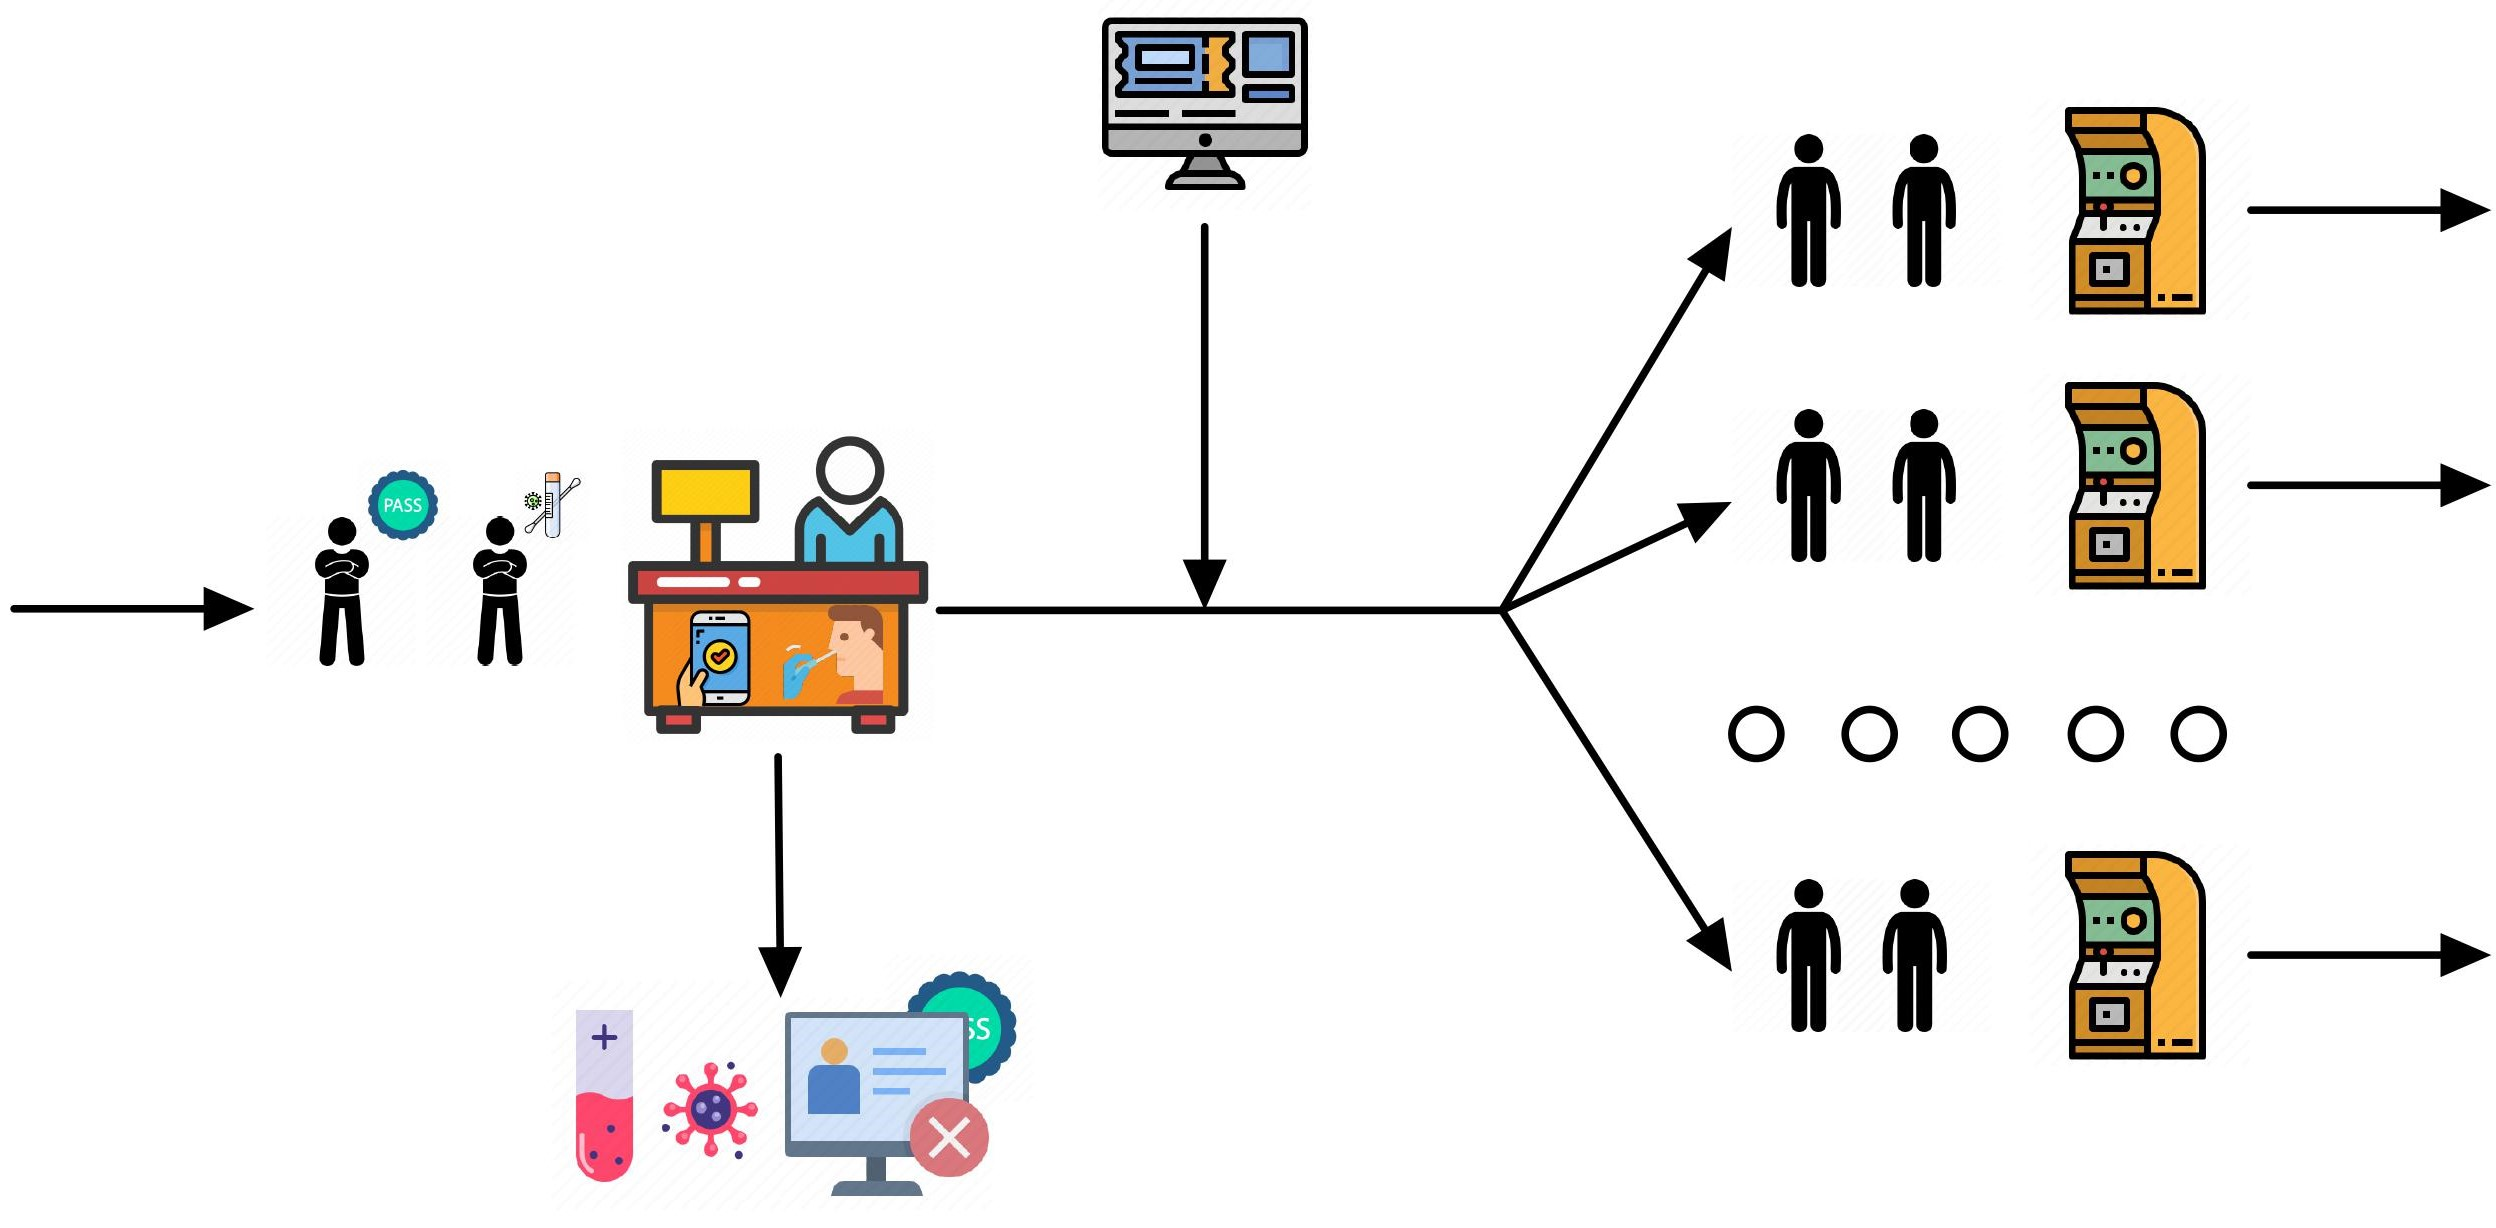
\includegraphics[scale=0.75]{images/base_model_high_level.jpg}
	\caption{Base Model, High-level view}\label{figura:base_model_high_level}
\end{figure}


%------------------------------------------------

\subsection{Obiettivi}
\label{Goal}
\par Il primo obiettivo dello studio è quello di massimizzare i profitti della sala giochi. A tale scopo è stata definita una funzione guadagno:

\begin{figure}[H]
	\centering
	\captionsetup{justification=centering,margin=2cm}
	
\includegraphics[scale=0.33]{images/base_income.png}
	\label{figura:adv_income}
\end{figure}

Il costo del biglietto è di 10 \euro . Per quanto riguarda l'elettricità è stata considerata una spesa giornaliera per Arcade pari a $2.4 €$ \euro. La funzione \textit{rimborso biglietto}, che calcola la percentuale del \textit{costo biglietto} da restituire al giocatore, è proporzionale al tempo di attesa speso da quest'ultimo in coda nei nodi Arcade. La massima percentuale rimborsabile è del $80\%$. L'attesa minima in coda per cui è previsto il rimborso è di 8 minuti. 
\\
\par Il secondo obiettivo dello studio è quello di assicurare un tempo medio di risposta del sistema inferiore a 40 minuti. Infatti, da un calcolo teorico basato sulle caratteristiche del sistema, specificate in seguito, si è dedotto che il tempo medio dei servizi del sistema è di circa 19 minuti. Per cui, è stata impostata una tolleranza del tempo medio di attesa nelle code sperimentato dall'utente, pari a circa il tempo di servizio.



	
%------------------------------------------------

\subsection{Modello Concettuale}
La sala giochi è modellata attraverso una rete aperta composta da N nodi rappresentanti i videogiochi e da un nodo rappresentante il controllo Covid-19. Ogni nodo si compone di un servente e di una coda infinita, poiché tale configurazione è la più verosimile.
\\
La struttura è aperta H24 e la giornata è suddivisa in 4 fasce orarie caratterizzate da tassi di arrivo differenti:
\begin{itemize}
\item 08:00-12:00
\item 12:00-17:00
\item 17:00-22:00
\item 22:00-08:00



\end{itemize}
Le variabili di stato del sistema considerate sono:
\begin{itemize}
\item Numero di clienti in ogni nodo;
\item Numero di nodi attivi;
\item Tipologia di cliente.
\end{itemize}
Le code inizialmente vengono considerate vuote, conseguentemente il numero di
clienti ad ogni nodo è 0. La tipologia di ogni cliente (Green-pass, tampone o biglietto online) è decisa aleatoriamente al suo arrivo. I nodi per ogni fase vengono definiti aperti o chiusi in base alla configurazione scelta durante lo studio, che può essere ottima o non
ottima.
\\ \\
Gli eventi considerati sono:
\begin{itemize}
\item Arrivo di un cliente;
\item Completamento di un servizio;
\item Cambio di fascia oraria.
\end{itemize}
Tali eventi possono causare cambiamenti dello stato. L’arrivo di un cliente causa
l’aumento della popolazione in un dato nodo e nel sistema. Il completamento di un servizio causa il passaggio di un cliente da un
nodo ad un altro o la sua uscita dal sistema. Il cambio di fascia oraria può causare
l’accensione o lo spegnimento degli Arcade. Se un nodo arcade viene spento quando ha ancora un cliente in servizio, questo continuerà a processarlo, pur non ricevendo altri
arrivi, mentre i clienti in coda vengono distribuiti uniformemente tra i nodi Arcade rimasti operativi. Il tempo in cui un nodo Arcade è idle, ma acceso, viene considerato nel calcolo dei
costi.
\par In figura \ref{figura:base_model_low_level} è possibile osservare lo schema a basso livello del modello base. 

\begin{figure}[H]
	\centering
	\captionsetup{justification=centering,margin=2cm}
	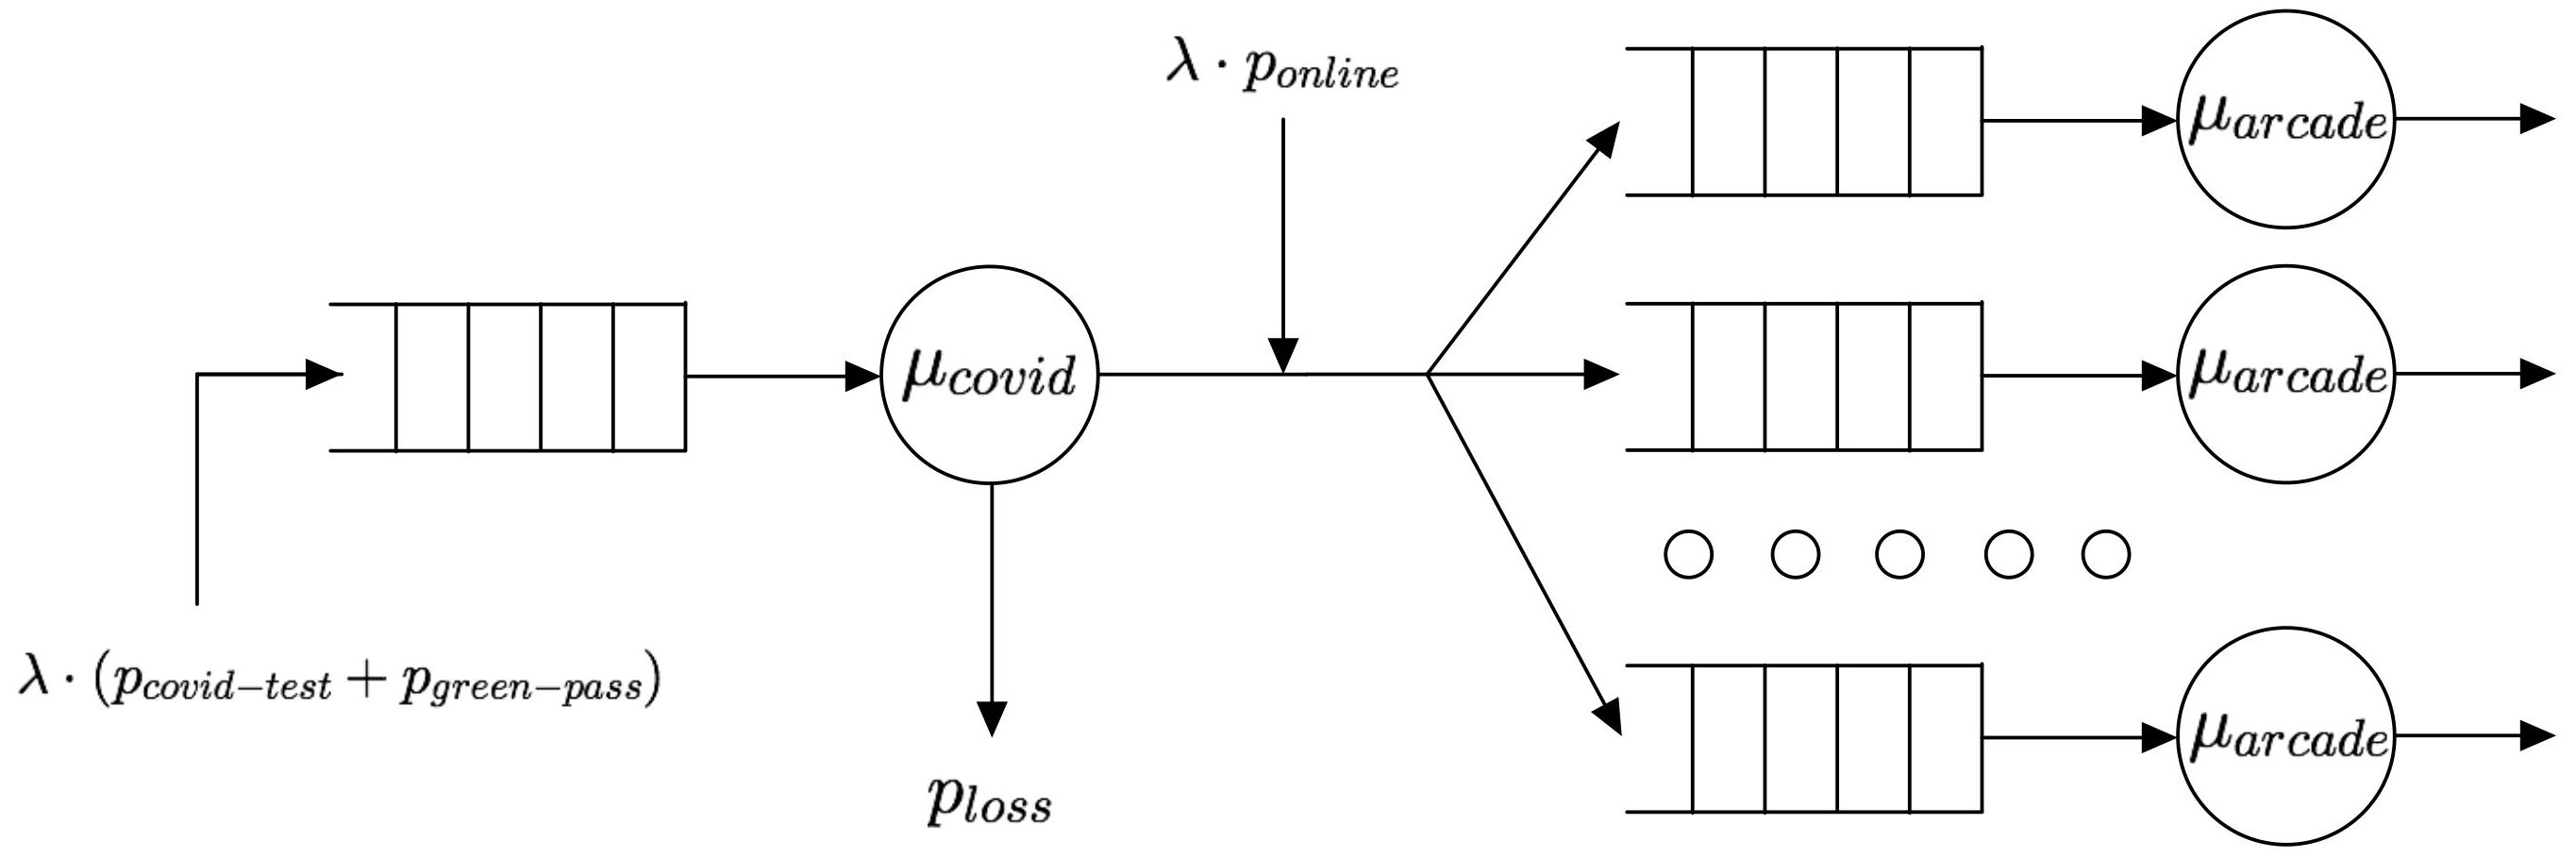
\includegraphics[scale=0.70]{images/base_model_low_level.jpg}
	\caption{Base Model, Low-level view}\label{figura:base_model_low_level}
\end{figure}


\subsection{Modello delle Specifiche}
Gli arrivi sono modellati con un processo di Poisson, con media variabile a seconda della fascia oraria. In particolare, la media per la prima fascia oraria è di $0.07143$  clienti/minuto (14 minuti/cliente), la media per la seconda fascia oraria è di $0.2$ clienti/minuto (5 minuti/cliente), la media per la terza fascia oraria è di $0.07143$ clienti/minuto (14 minuti/cliente), la media per la quarta fascia oraria è di $0.02857$  clienti/minuto (35 minuti/cliente).
\\ \\
La percentuale di clienti con biglietto online è del 20\%. La percentuale di clienti che si sottopone al controllo del  Green-pass è del 48\%. La percentuale di clienti che si sottopone al tampone è del 32\%.
\\ \\
La distribuzione del tempo di servizio per il controllo del green-pass è stata modellata
con una distribuzione Normale con media 2 minuti (0.5 clienti/minuto) e varianza 2.25 minuti, troncata tra 1 e 3 minuti. 
\\
La distribuzione del tempo di servizio per il tampone è stata modellata
con una distribuzione Normale con media 10 minuti (0.1 clienti/minuto) e varianza 2.25 minuti, troncata tra 8 e 12 minuti. 
\\
È stata scelta una Normale troncata con questi valori poiché permette di modellare un'operazione con bassa variabilità e di scartare valori eccessivamente piccoli o grandi che non rispecchierebbero tempi di servizio reali.
\\ \\
La distribuzione del tempo di servizio per un generico arcade è stata modellata
con una distribuzione Normale con media 15 minuti ($0.0\overline{6}$ clienti/minuto) e varianza 9 minuti, troncata tra 3 e 25 minuti.
\\ \\
La percentuale di clienti che risulta positiva al Covid-19 oppure presenta un green-pass non idoneo è in totale del 5\%.
\\ \\
Le probabilità per la scelta del node arcade è stata modellata tramite una distribuzione Uniforme in modo che ciascun servente abbia la stessa probabilità di essere selezionato. Questa scelta permette di mantenere circa la stessa utilizzazione per tutti i serventi dato che hanno lo stesso tasso di servizio.
\\ \\
Infine, si considera un numero di nodi per il controllo Covid-19 pari a 1 ed un numero massimo di nodi arcade pari a 20.


\subsection{Modello Computazionale}
L’approccio di simulazione utilizzato è stato quello Next-Event Simulation. Il linguaggio di programmazione utilizzato è \textit{Python v.3.8}, facendo particolare riferimento alle librerie \ref{link} implementate dall’autore del libro di testo, e forniteci nel corso delle lezioni.
Il codice di base per la simulazione segue quanto descritto nell'algoritmo \ref{algo1}. Quest'ultimo si avvale di ulteriori strutture dati e funzioni necessarie al corretto funzionamento.

\begin{algorithm}[H]
\caption{Rete Aperta - Scheduling FIFO}\label{algo1}
\begin{algorithmic}[1]
\Procedure{Modello Base}{}
\State $\textit{Inizializzazione clock}$
\State $\textit{Inizializzazione lista dei nodi}$
\State $\textit{Inizializzazione struttura Integrali}$
\State $\textit{Selezione nodo su cui generare il primo arrivo}$
\State $\textit{Generazione primo arrivo}$
\While{\textit{ultimo arrivo $<$ STOP} \textbf{or} \textit{ci sono job nel sistema}}
  \State $\textit{Scelta del prossimo evento}$
  \For{$i\gets 0, \textit{numero nodi}$}
    \If{$\textit{nodi non vuoti}$}
      \State $\textit{Aggiornamento statistiche}$
    \EndIf

  \EndFor
  \State $\textit{Avanzamento del clock}$
  \If{\textit{Evento} $= \textit{Cambio fascia oraria}$}
  \State $\textit{Selezione tasso arrivi corretto}$
  \EndIf
  \If{\textit{Evento} $= Arrivo$} \Comment{Arrivo}
    \State $\textit{Aggiornamento stato nodo}$
    \State $\textit{Aggiornamento stato sistema}$
    \State $\textit{Schedulazione prossimo arrivo}$
    \If{\textit{Jobs nel centro} $= 1$}
      \State $\textit{Schedulazione prossimo servizio}$
    \EndIf
  \Else  \Comment{Completamento}
    \State $\textit{Aggiornamento stato nodo}$
    \If{\textit{Nodo Arcade}}
      \State $\textit{Aggiornamento stato sistema}$
    \EndIf
    \If{\textit{Jobs nel centro} $> 0$}
      \State $\textit{Schedulazione prossimo servizio}$
    \EndIf
    \If{\textit{Nodo Covid-Check}}
      \If{\textit{Covid test negativo }\text{\textbf{and}} \textit{Green-pass valido}}
        \State $\textit{Aggiornamento stato sistema}$
      \EndIf
    \EndIf
  \EndIf
\EndWhile
\EndProcedure
\end{algorithmic}
\end{algorithm}


\subsection{Verifica}
Le strutture e le funzioni precedentemente accennate sono state sottoposte ad una fase di testing in modo da garantire il loro corretto funzionamento. Durante l'implementazione del progetto, l'applicazione iterativa di tale fase ha permesso di individuare e correggere diversi difetti, emersi a seguito del manifestarsi di malfunzionamenti del sistema.

\subsection{Validazione}
Al fine di validare il modello implementato, sono stati eseguiti diversi run variando determinati parametri. I risultati possono essere osservati in tabella \ref{tab1} e \ref{tab2}.

\begin{table}[htbp]
\caption{System statistics}
\begin{center}
\begin{tabular}{|c|c|c|c|}
\hline
\textbf{\# nodi arcades} & \textbf{avg interarrival time} & \textbf{avg wait} & \textbf{avg \# node} \\ \hline
\textbf{2} & 14.037119 & 27.6247051 & 1.967967 \\ \hline
\textbf{5} & 14.037119 & 21.808119 & 1.553597 \\ \hline
\textbf{9} & 14.037119 & 20.885323 & 1.487860 \\ \hline
\multicolumn{4}{l}{$^{\mathrm{*}}$ $seed=1234567891, \lambda_{system} =\frac{1}{14} \frac{job}{min}, \# jobs=517028, $}
\end{tabular}
\label{tab1}
\end{center}
\end{table}

Per quanto riguarda la tabella \ref{tab1}, è possibile evincere come il tempo di interarrivo medio del sistema converga al parametro impostato $\lambda_{system}^{-1}$.


\begin{table}[htbp]
\caption{Arcade statistics}
\begin{center}
\begin{tabular}{|c|c|c|c|c|c|c|}
\hline
\textbf{\# nodi arcades} & \textbf{avg interarrival time} & \textbf{avg wait} & \textbf{avg delay} & \textbf{avg \# node} & \textbf{avg \# queue} & \textbf{utilization} \\ \hline
\textbf{2} & 29.243586 & 23.024591 & 8.028968 & 0.787335 & 0.274554 & 0.512781\\ \hline
\textbf{5} & 73.123549 & 16.937644 & 1.940329 & 0.231630 & 0.026538 & 0.205092\\ \hline
\textbf{9} & 131.750016 & 15.999674 & 0.983205 & 0.121439 & 0.007463 & 0.113977\\ \hline
\multicolumn{7}{l}{$^{\mathrm{*}}$ $seed=1234567891, \lambda_{system} =\frac{1}{14} \frac{job}{min}, \# jobs=517028, $}
\end{tabular}
\label{tab2}
\end{center}
\end{table}


Per quanto riguarda la tabella \ref{tab2}, si può notare come la relazione di Little, applicabile in quanto il modello soddisfa le condizioni sufficienti, sia soddisfatta e come l'utilizzazione e il tempo di interarrivo medio, rispettivamente, decresca ed aumenti al crescere del numero degli arcade. Tale comportamento è giustificato dal fatto che i jobs vengono distribuiti in modo equiprobabile tra i diversi nodi arcade.
\\ \\
Come è possibile osservare dalle tabelle, inoltre, all'aumentare dei nodi nel sistema i tempi di attesa e il numero di jobs nei rispettivi centri diminuisce coerentemente a ciò che ci si aspetta.

\subsection{Esperimenti di Simulazione}
%----Introduzione
Al fine di raggiungere gli obiettivi prefissati, è utile dedurre il minimo numero di nodi che permette al sistema di raggiungere la stazionarietà e, in seguito, ricavare la configurazione ottimale del sistema.

Il raggiungimento della stazionarietà o meno viene studiato attraverso l'impiego dell'analisi a orizzonte finito, mentre quella a orizzonte infinito permette di confrontare le configurazioni del sistema a partire dai risultati ottenuti dal comportamento transiente. 
\subsubsection{Analisi del comportamento transiente}
%----Minimo n per stazionarietà
Attraverso l'analisi del comportamento transiente viene studiato il tempo medio di risposta del sistema, per ogni fascia oraria, utilizzando il metodo delle repliche.
In particolare, vengono effettuati run di simulazione
consecutivi, utilizzando ogni volta come punto di partenza lo stato del sistema raggiunto dalla replica precedente. Il seed, infatti, viene settato una volta, all'inizio della prima replica.
La tecnica delle repliche permette di calcolare stime puntuali e intervallari ad ogni acquisizione, ognuna di queste corrispondente ad un certo numero di richieste processate.

Una prima analisi ha portato ad osservare che il sistema non può raggiungere la stazionarietà per via dei limiti introdotti dalla coda del controllo Covid-19, essendo unica per modellazione. Infatti, per un $\lambda_{arrival} \gtrsim \frac{1}{4.1}$, l'utilizzazione di tale centro è approssimativamente pari ad 1, mentre quella dei centri Arcade risulta essere inferiore. Questo studio permette di concludere che il collo di bottiglia è rappresentato dalla coda del controllo Covid-19, per questo motivo, segue solamente lo studio dei nodi Arcade, considerando un $\lambda_{arrival} < \frac{1}{4.1}$.
\\ \\
Per quanto riguarda la prima fascia e la terza fascia oraria, rispettivamente (08:00-12:00) e (17:00-22:00), è possibile osservare i risultati dell'analisi in figura \ref{figura:avg_ws_mor_ns} e figura \ref{figura:avg_ws_mor_s}. Tali fasce, infatti, hanno lo stesso $\lambda_{arrival}$ da modellazione.

\begin{figure}[H]
\centering
\captionsetup{justification=centering,margin=2cm}
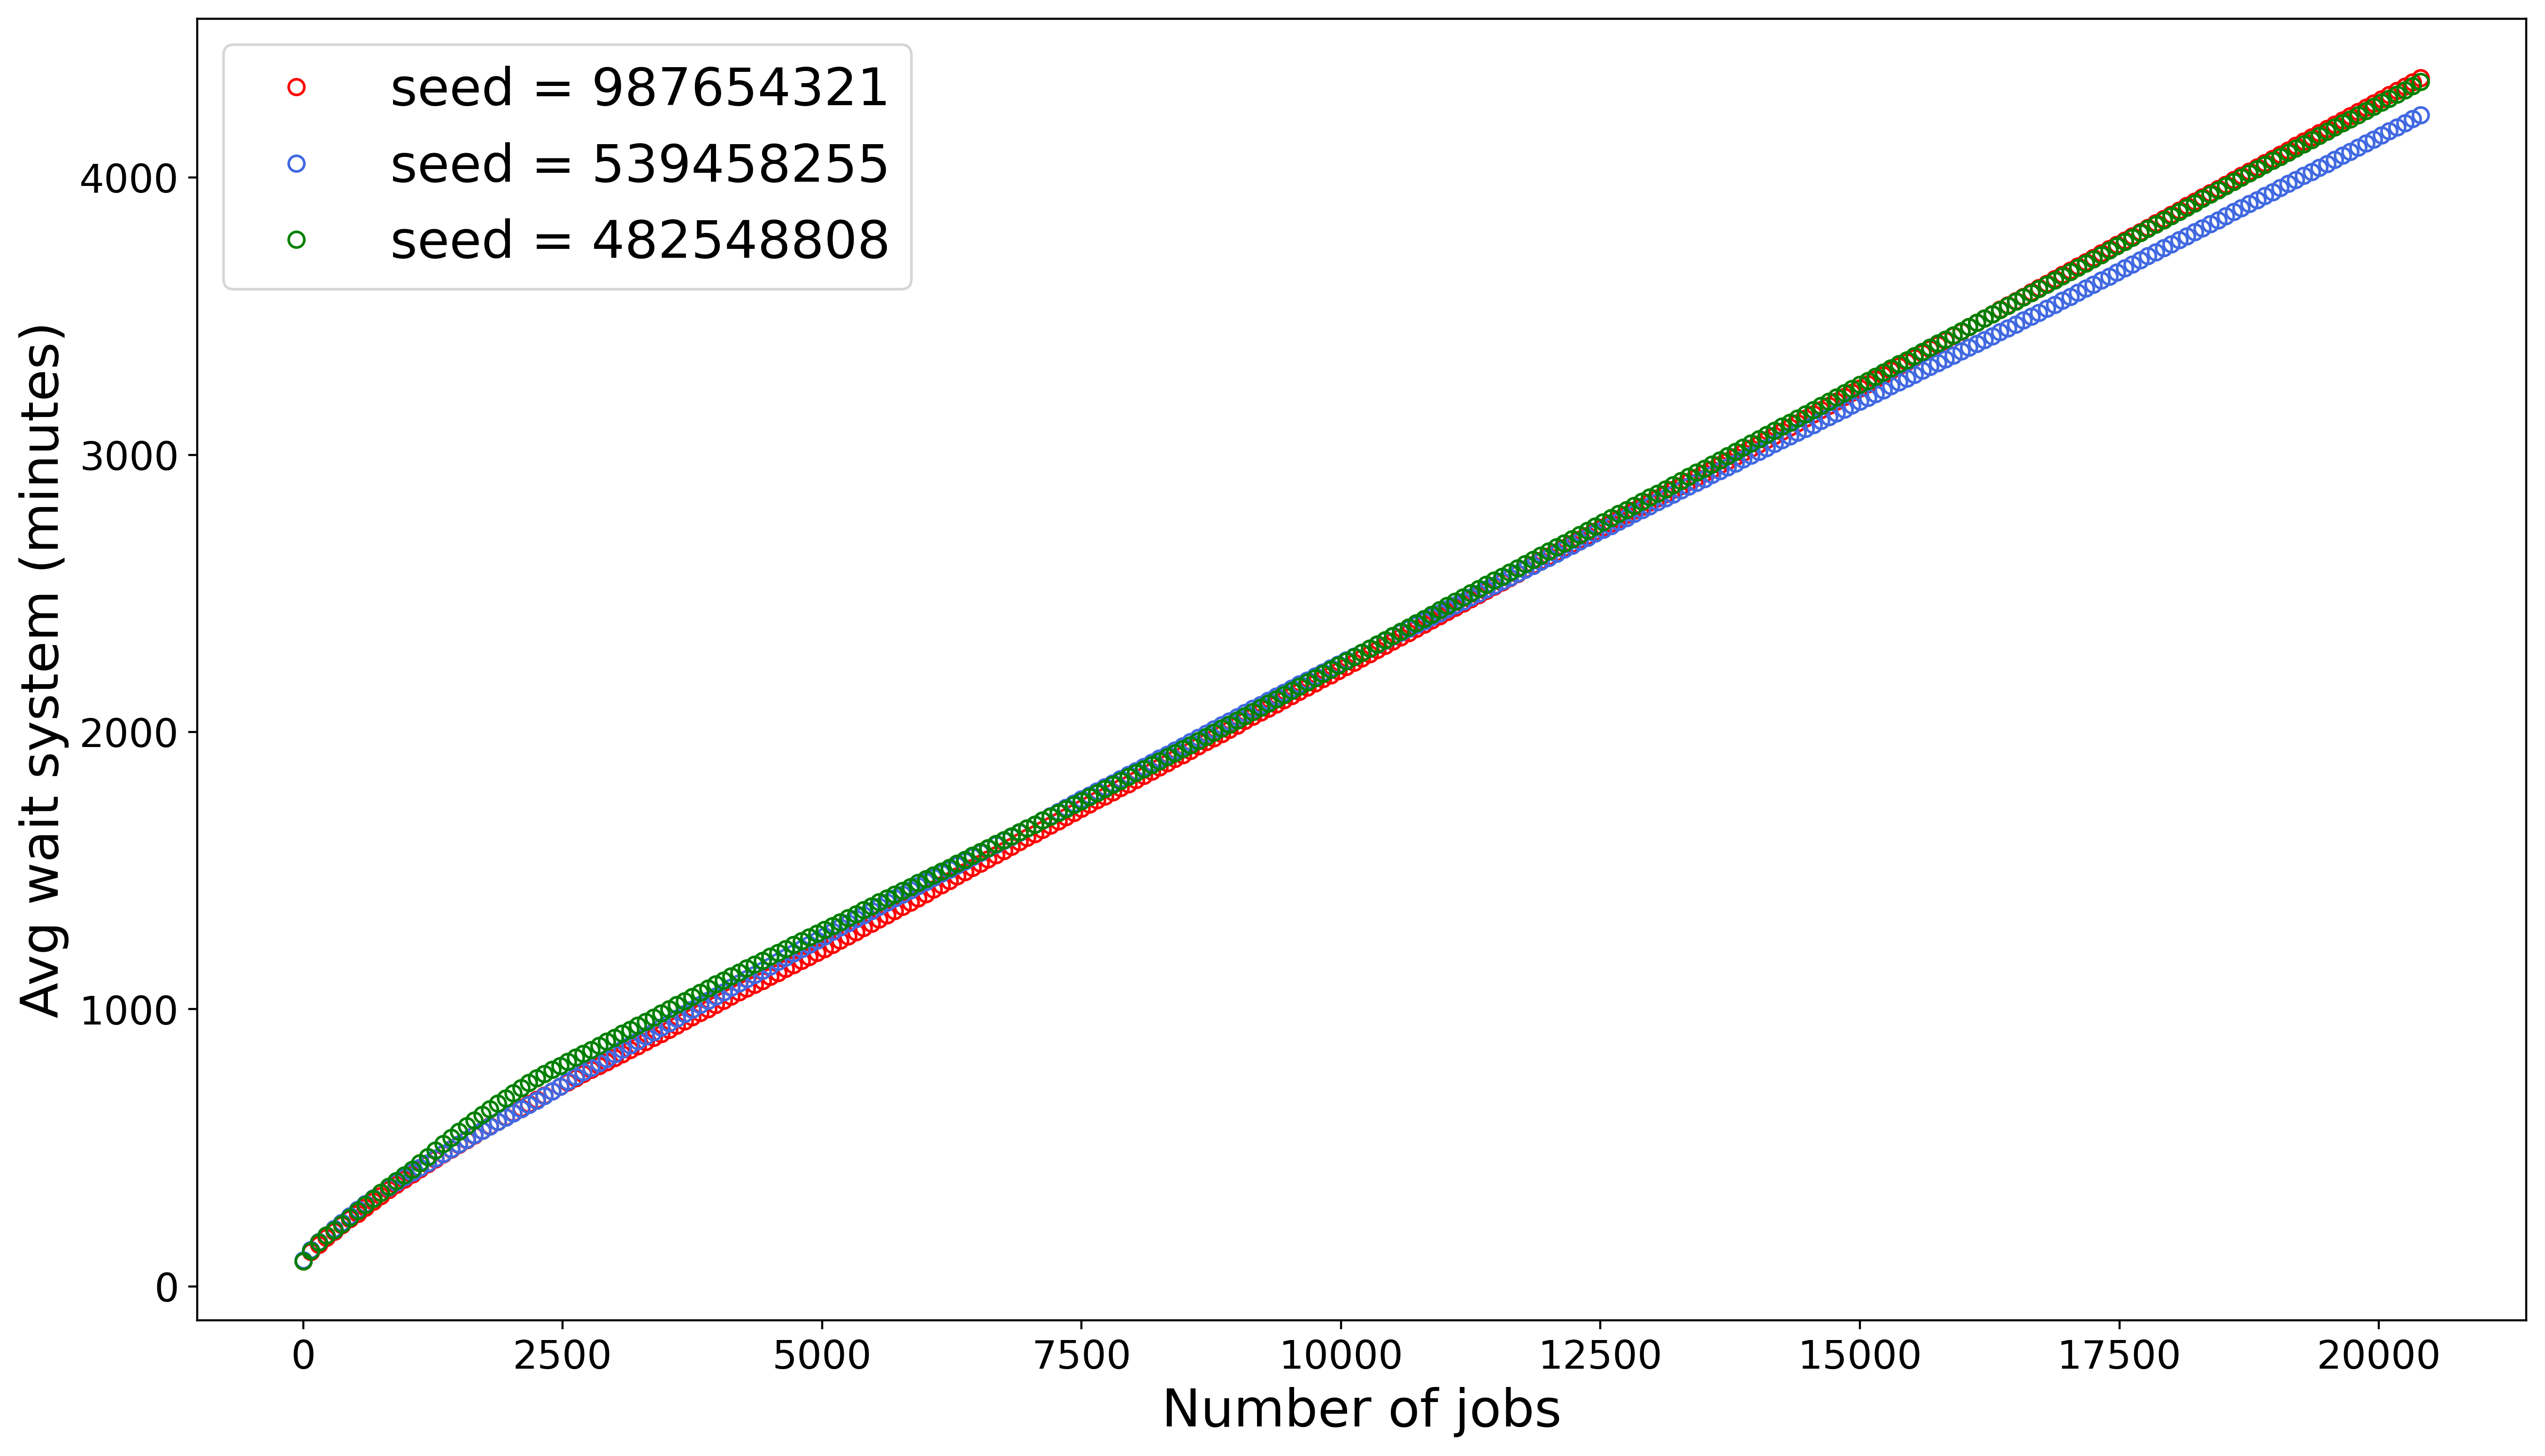
\includegraphics[scale=0.48]{images/transient_mor_ns.png}
\caption{Average Wait System, 08:00-12:00 \& 17:00-22:00, $\lambda_{arrival}=\frac{1}{14} \frac{job}{min}$, Arcades: 1, repliche=64, Sampling\_freq=75}\label{figura:avg_ws_mor_ns}
\end{figure}
\begin{figure}[H]
\centering
\captionsetup{justification=centering,margin=2cm}
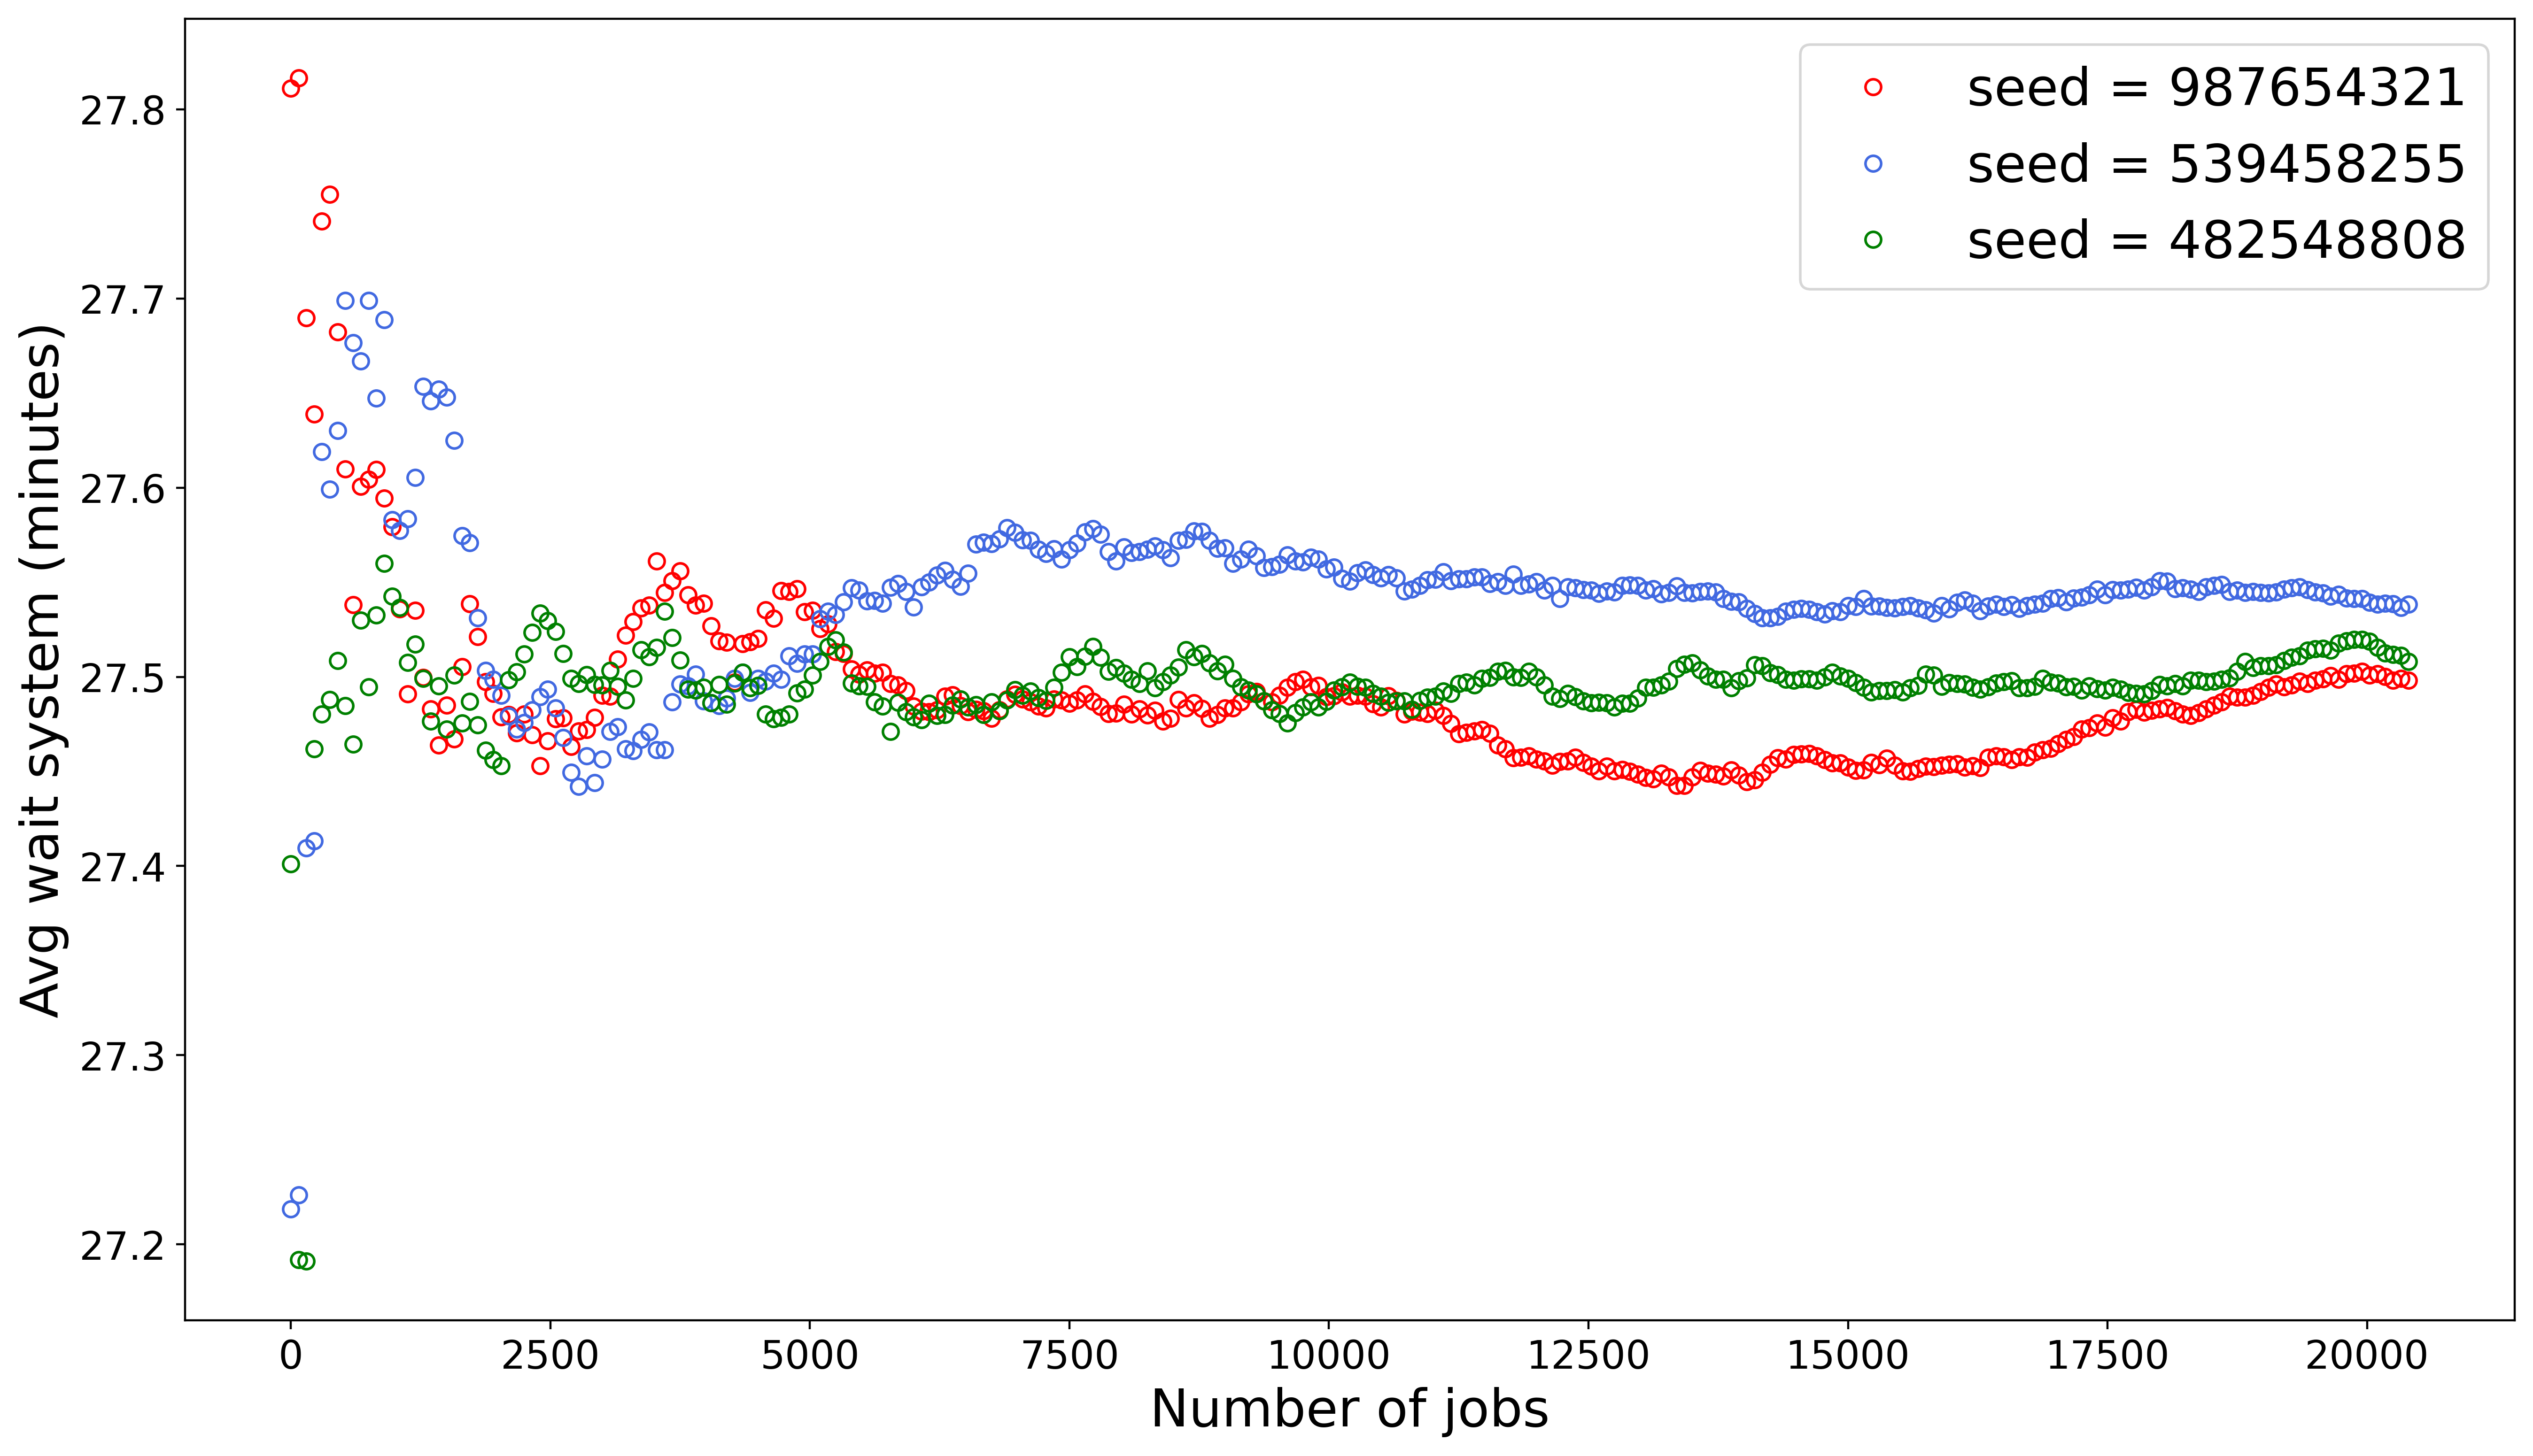
\includegraphics[scale=0.48]{images/transient_mor_s.png}
\caption{Average Wait System, 08:00-12:00 \& 17:00-22:00, $\lambda_{arrival}=\frac{1}{14} \frac{job}{min}$, Arcades: 2, repliche=64, Sampling\_freq=75}\label{figura:avg_ws_mor_s}
\end{figure}

Come si evince dai grafici, il numero minimo di nodi Arcade necessari per il raggiungimento della stazionarietà, nella fascia oraria 08:00-12:00 e 17:00-22:00, è pari a 2. Infatti, nella figura \ref{figura:avg_ws_mor_s} il tempo medio di risposta del sistema assume un comportamento stabile dopo il processamento di circa $5000$ jobs. Inoltre, sono stati utilizzati 3 seed iniziali diversi, in modo tale da simulare il comportamento in condizioni aleatorie differenti. Tali considerazioni, con le dovute differenze, valgono per le altre fasce orarie.
\\ \\
Per quanto riguarda la seconda fascia oraria (12:00-17:00), è possibile osservare i risultati dell'analisi in figura \ref{figura:avg_ws_aft_ns} e figura \ref{figura:avg_ws_aft_s}.




\begin{figure}[H]
\centering
\captionsetup{justification=centering,margin=2cm}
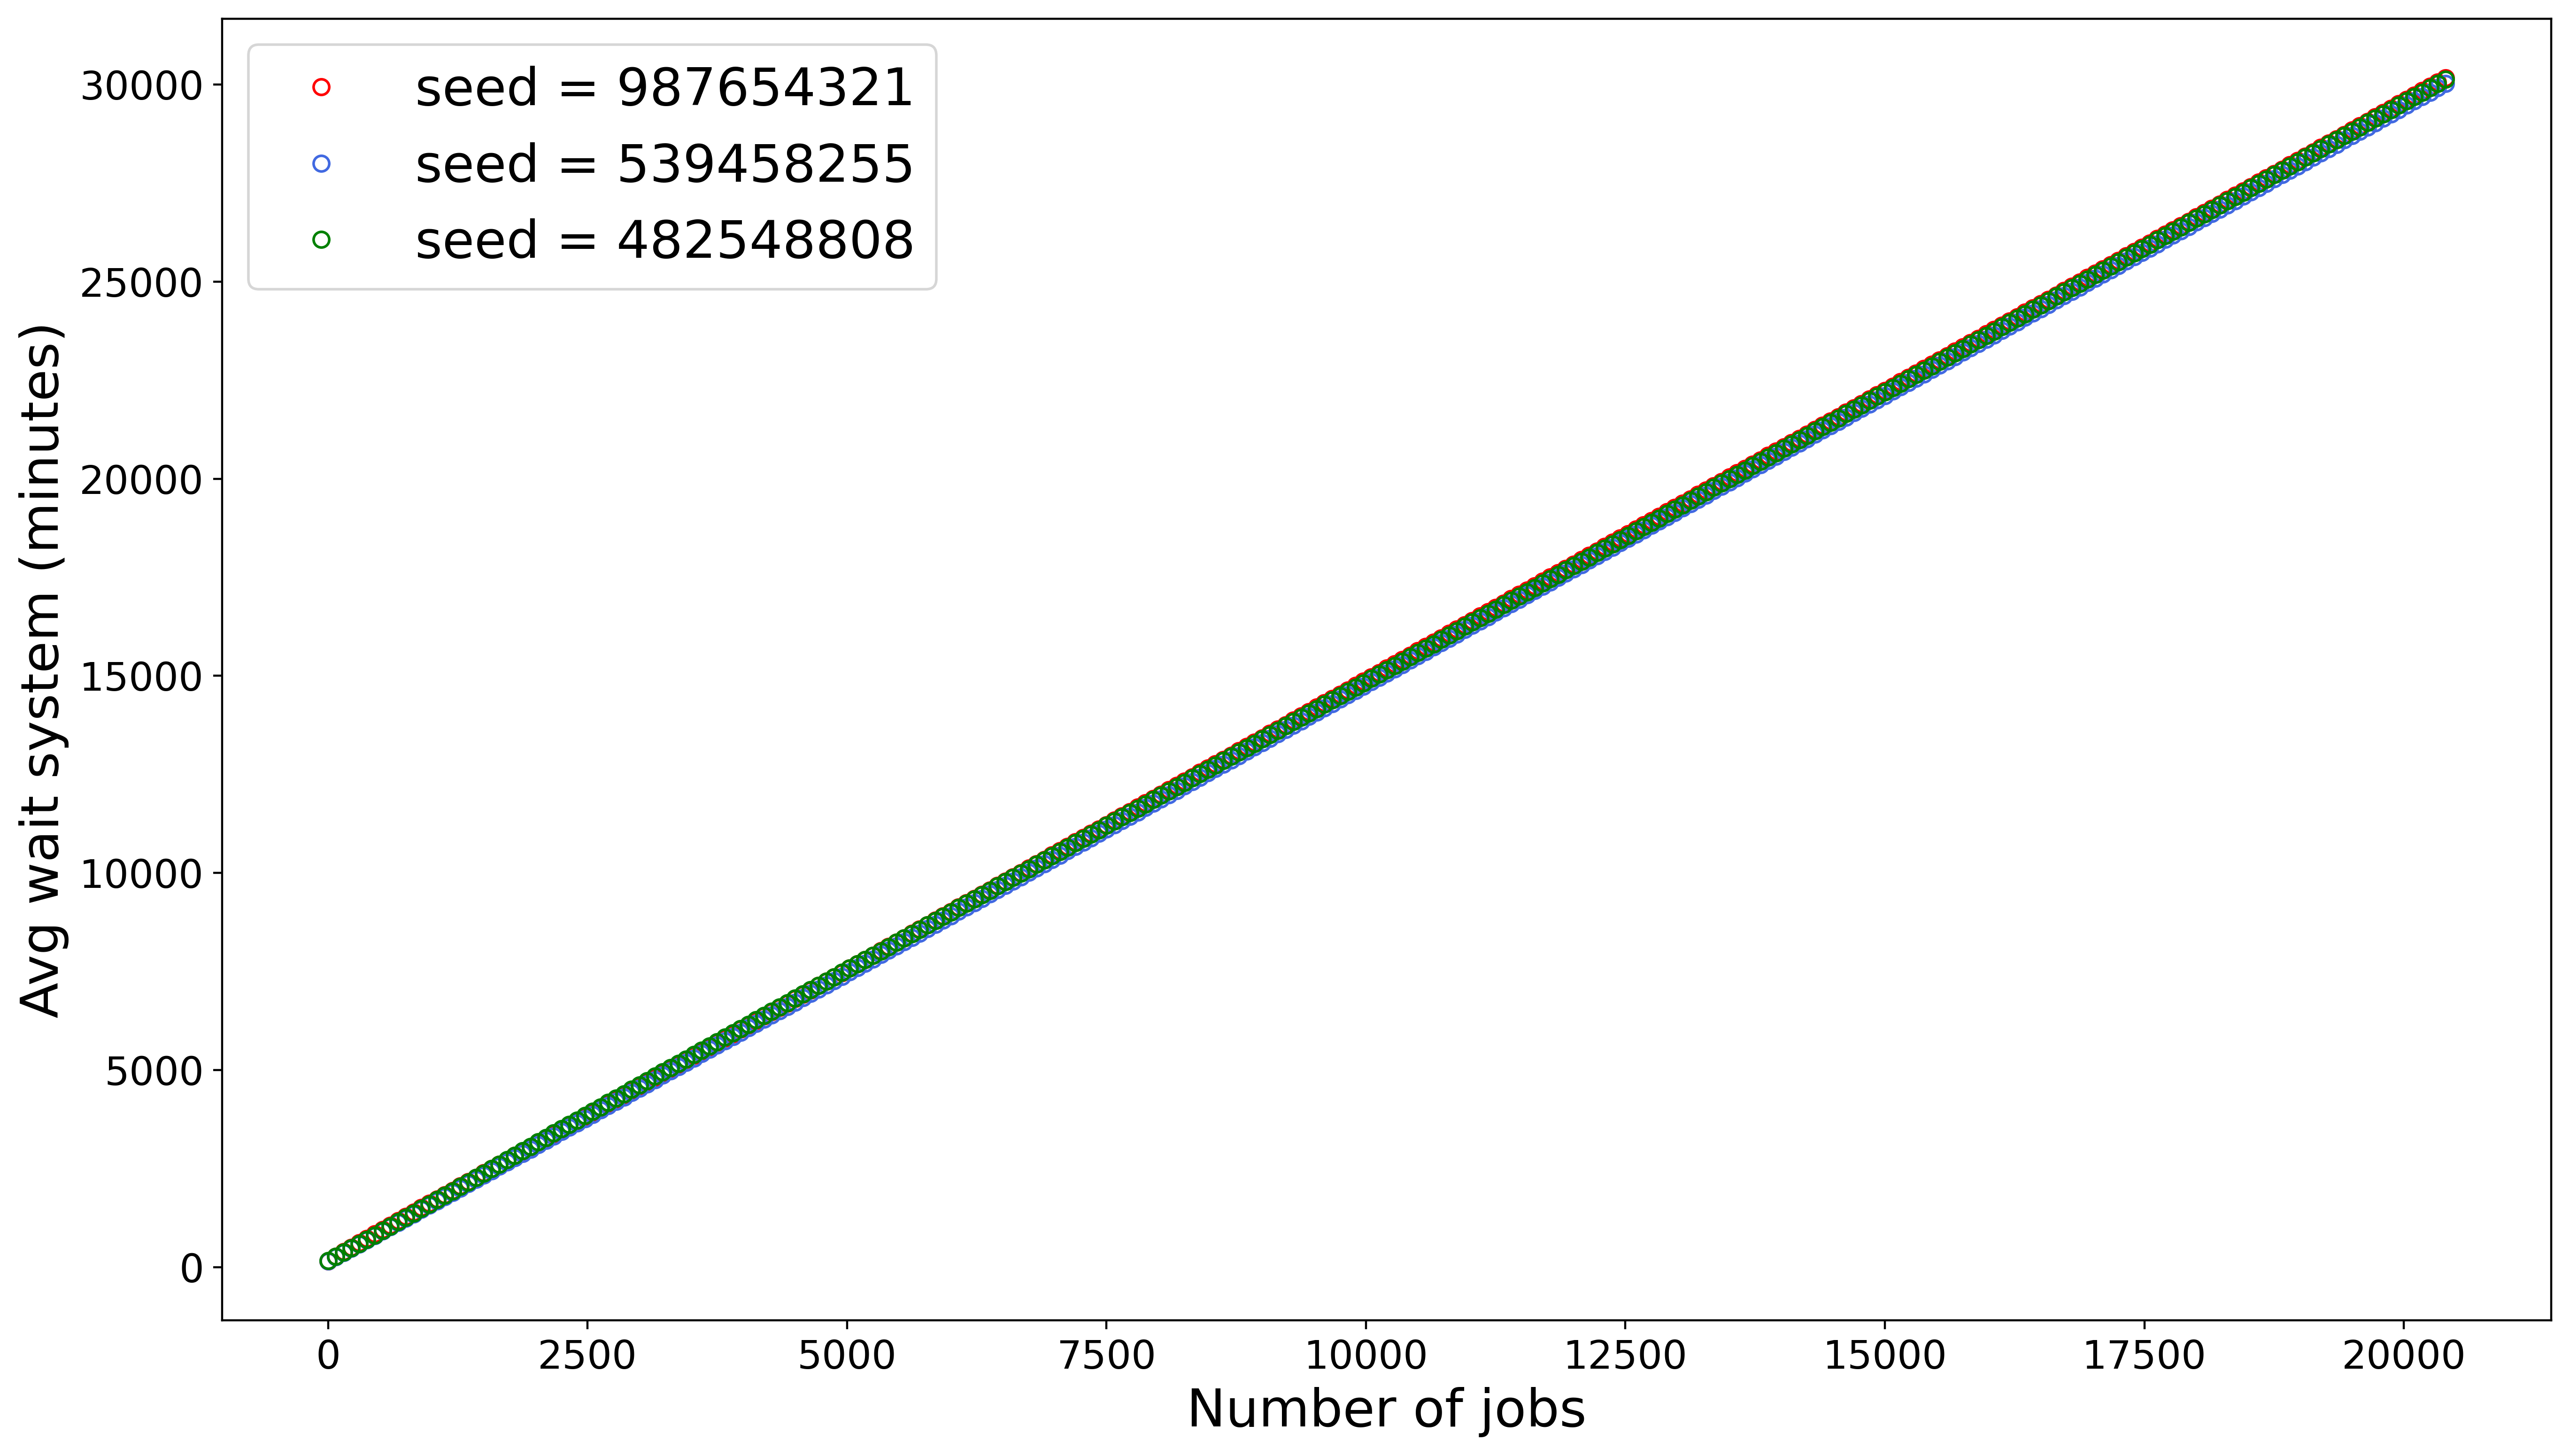
\includegraphics[scale=0.48]{images/transient_aft_ns.png}
\caption{Average Wait System, 12:00-17:00, $\lambda_{arrival}=\frac{1}{5} \frac{job}{min}$, Arcades: 2, repliche=64, Sampling\_freq=75}\label{figura:avg_ws_aft_ns}
\end{figure}
\begin{figure}[H]
\centering
\captionsetup{justification=centering,margin=2cm}
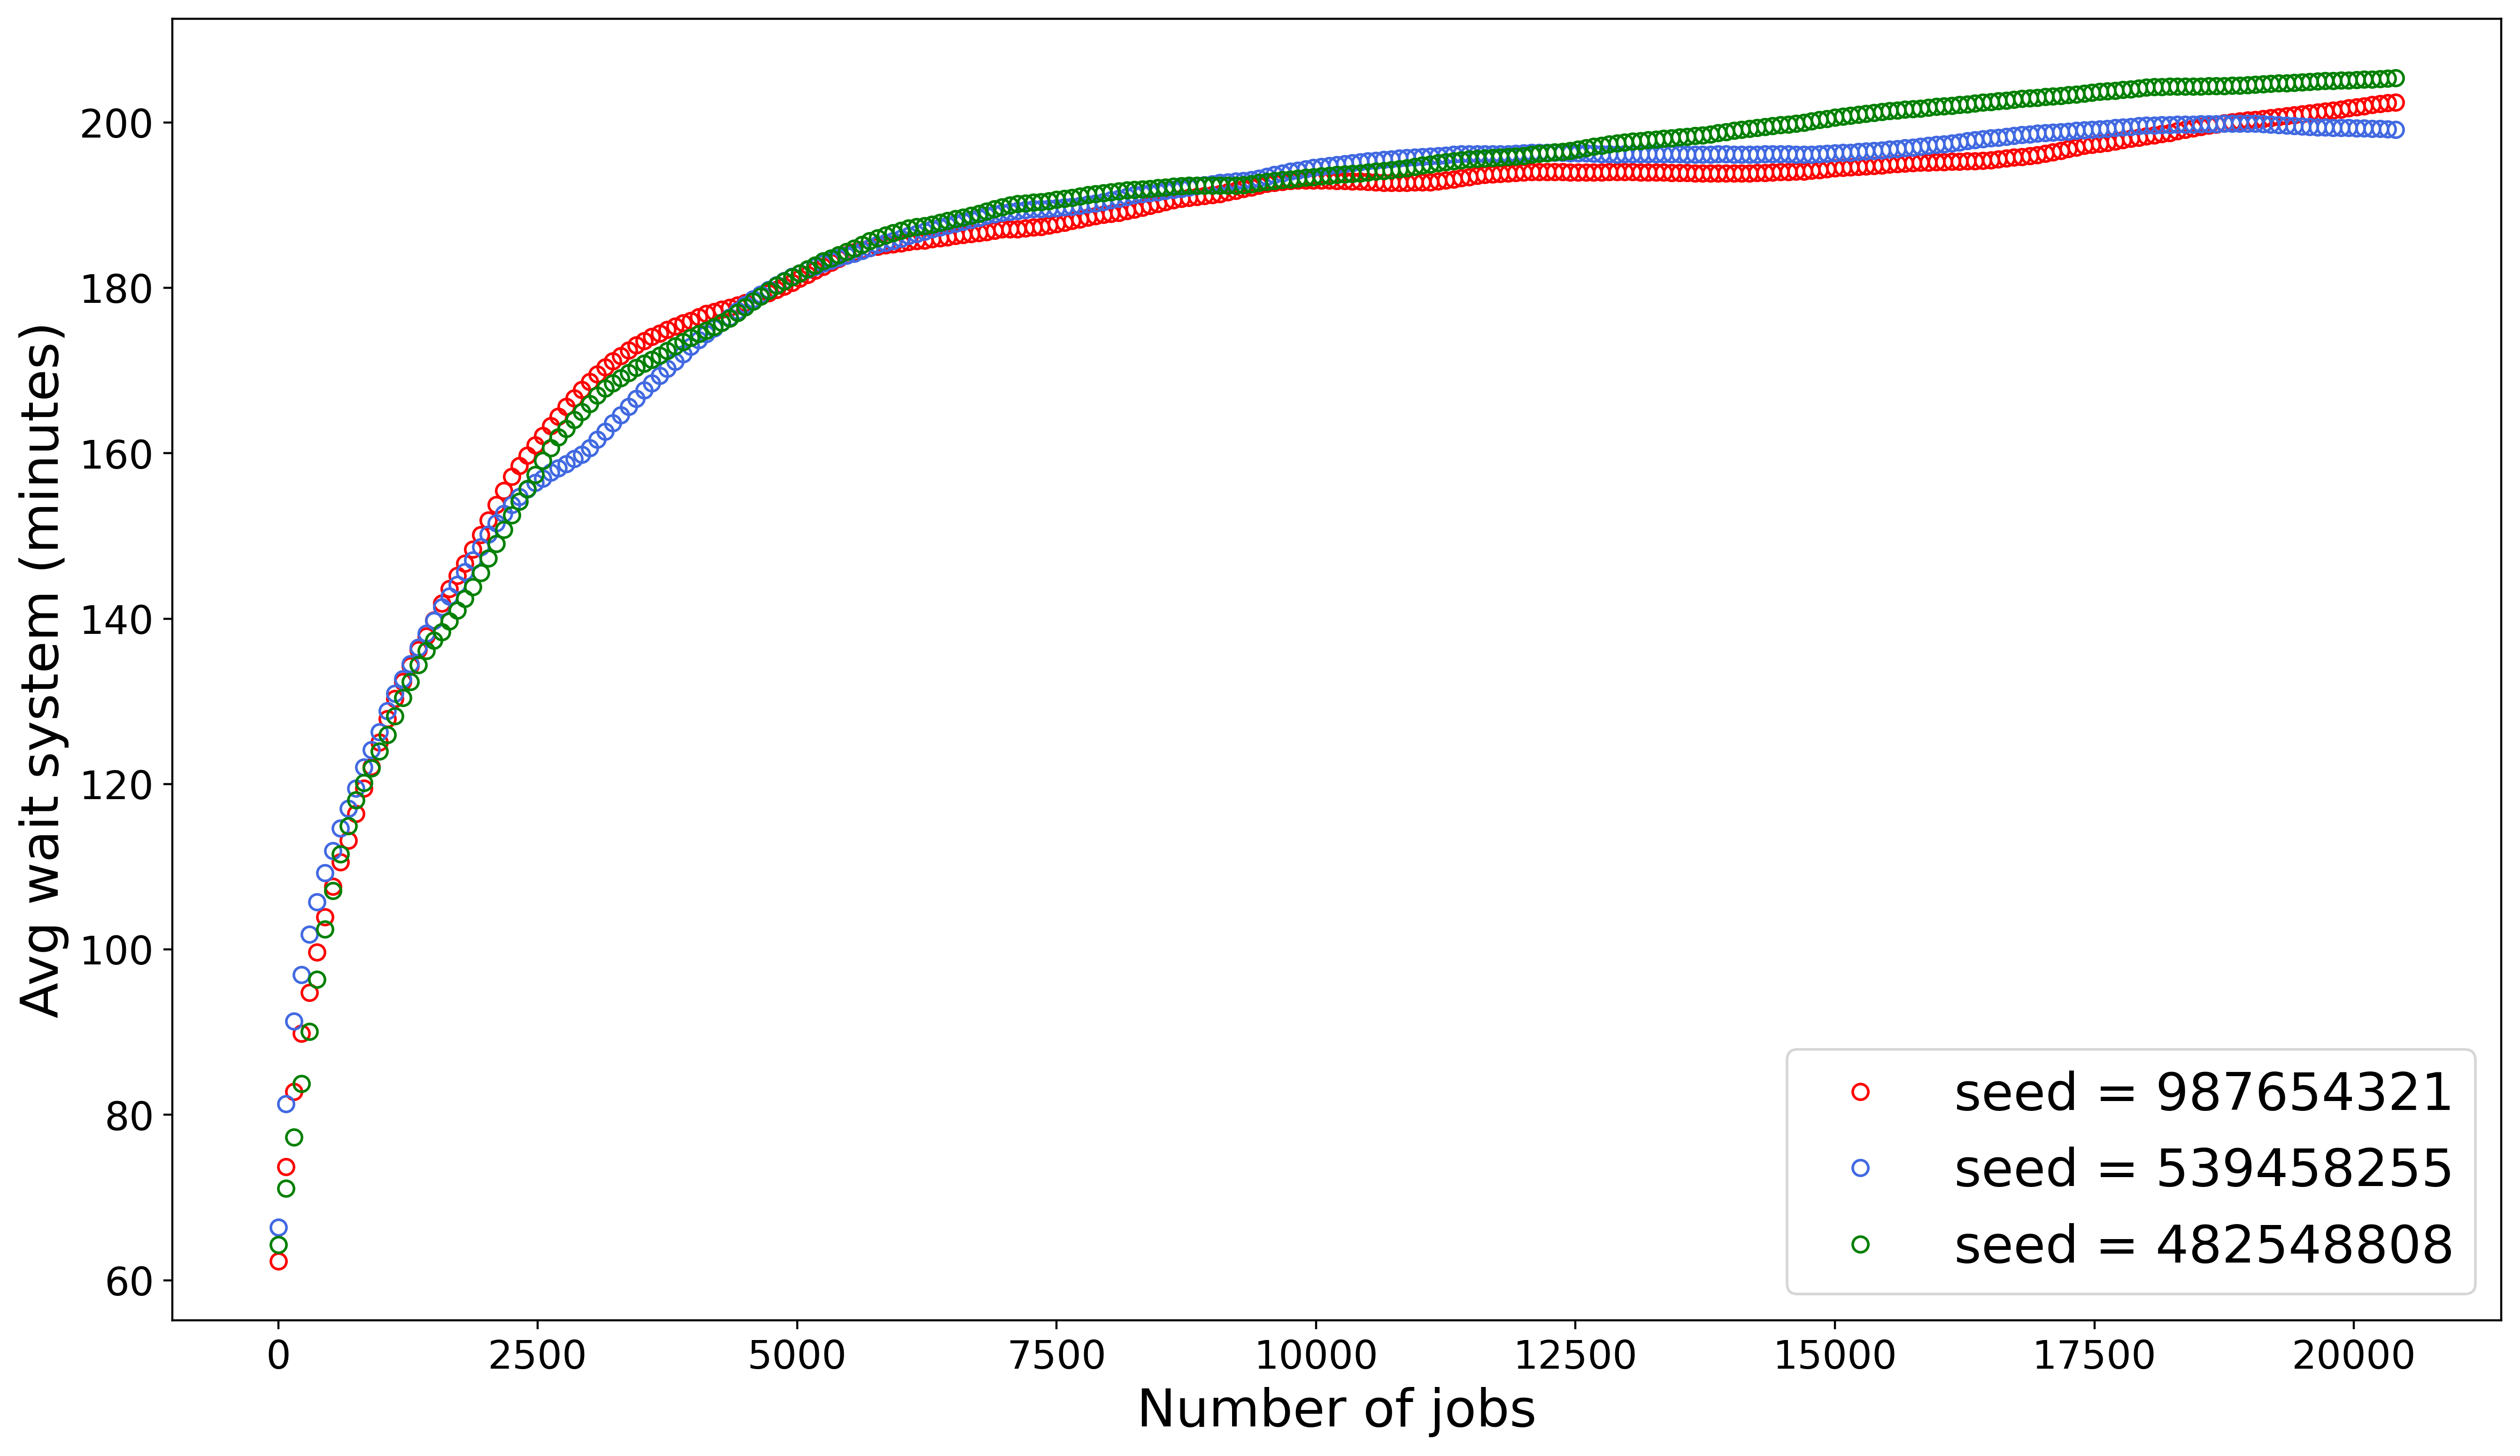
\includegraphics[scale=0.48]{images/transient_aft_s.png}
\caption{Average Wait System, 12:00-17:00, $\lambda_{arrival}=\frac{1}{5} \frac{job}{min}$, Arcades: 3, repliche=64, Sampling\_freq=75}\label{figura:avg_ws_aft_s}
\end{figure}


Per quanto riguarda la quarta fascia oraria (22:00-08:00), è possibile osservare i risultati dell'analisi in figura \ref{figura:avg_ws_night_s}.


\begin{figure}[H]
\centering
\captionsetup{justification=centering,margin=2cm}
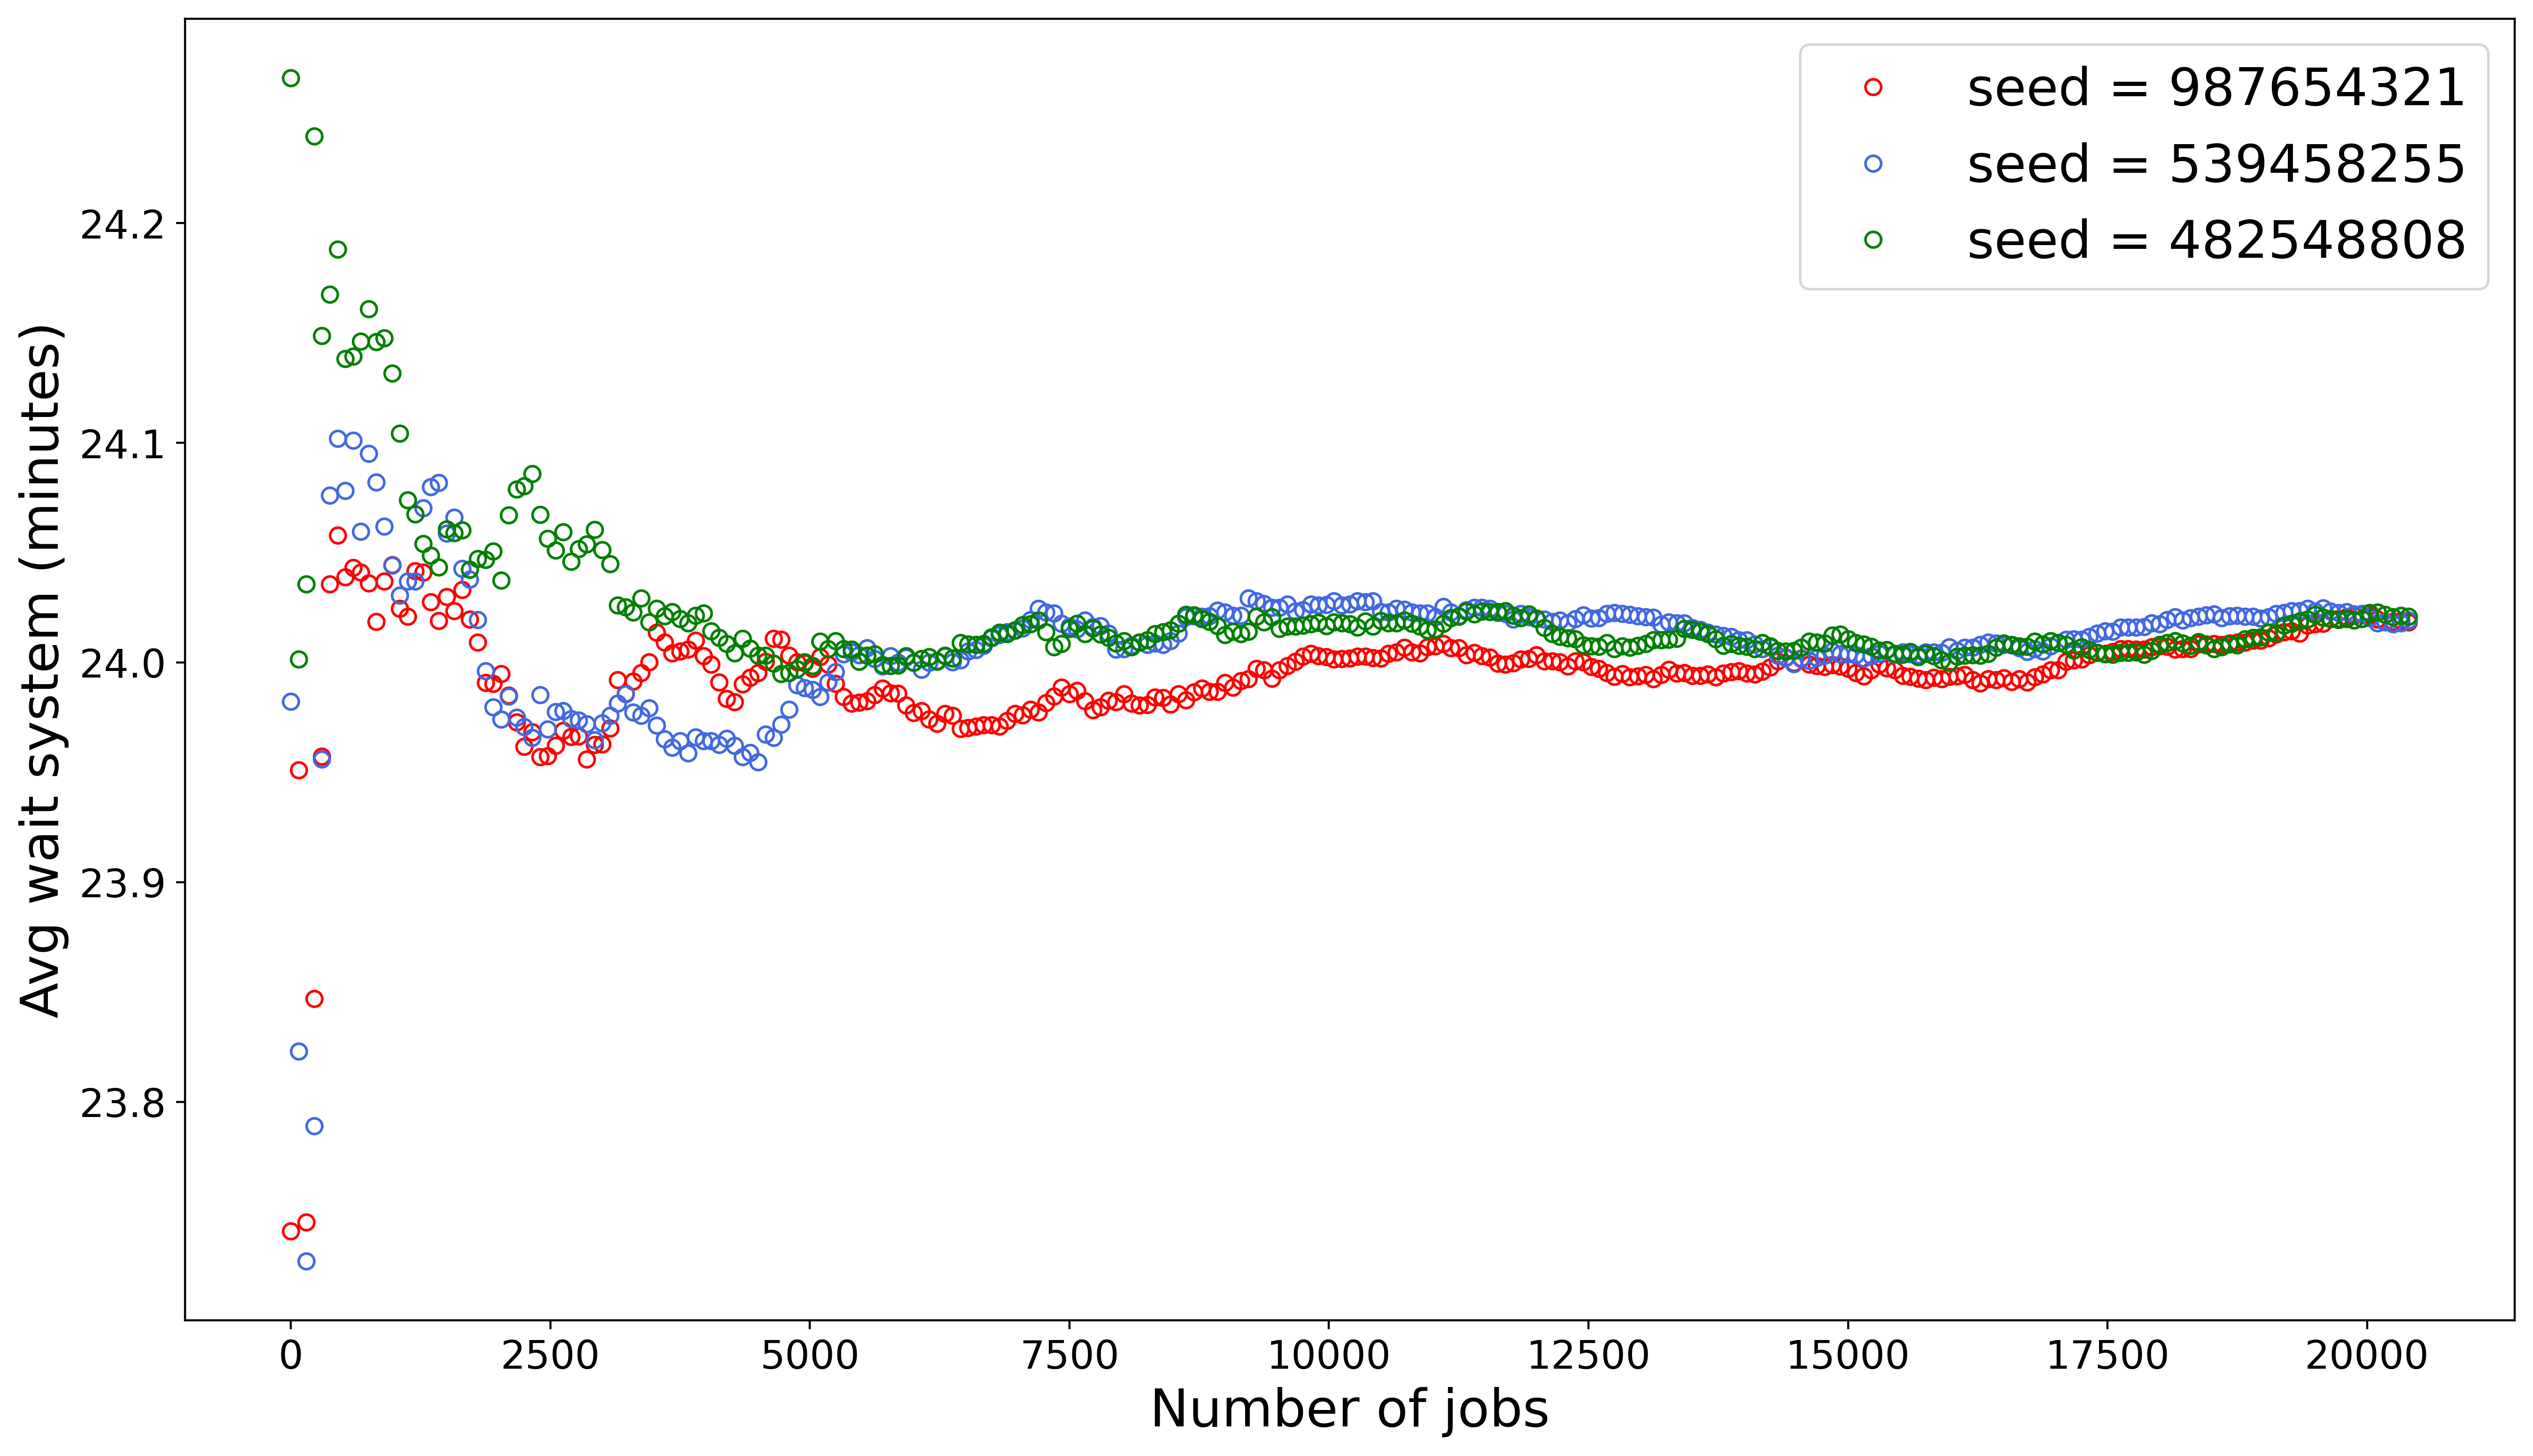
\includegraphics[scale=0.48]{images/transient_night_s.png}
\caption{Average Wait System, 22:00-08:00, $\lambda_{arrival}=\frac{1}{35} \frac{job}{min}$, Arcades: 1, repliche=64, Sampling\_freq=75}\label{figura:avg_ws_night_s}
\end{figure}

In questo caso, il tempo di risposta medio del sistema si stabilizza anche con l'utilizzo di un solo nodo Arcade.

\subsubsection{Analisi del comportamento stazionario}
%----Massimizzazione del guadagno
Considerati i risultati dell'analisi transiente, è possibile procedere allo studio del comportamento stazionario.
Attraverso l'analisi del comportamento stazionario si vuole trovare la configurazione ottima di nodi arcade, per ogni fascia oraria, che permetta di raggiungere gli obiettivi prefissati in \ref{Goal}, partendo dai risultati ottenuti dallo studio precedente.
In questa fase sono state effettuate simulazioni con tempi
d’osservazione molto lunghi, utilizzando la tecnica batch-means per ottenere delle stime degli indici di prestazione in regime stazionario, evitando la problematica del bias dovuto alle condizioni iniziali del sistema. Cruciale in questa fase la scelta di due parametri: \textit{b} e \textit{k}, rispettivamente la grandezza del batch e il numero di batch in cui si divide la simulazione. Per la scelta di \textit{b} è stata utilizzata la linea guida di Banks, Carson, Nelson, e Nicol (2001), la quale afferma che il batch size venga aumentato fintantoché l'autocorrelazione a lag 1 tra i batch sia minore di 0.2. Nel caso in esame è stato constatato che tale direttiva viene rispettata con un \textit{b} pari a 256. Per la scelta del parametro \textit{k} è stato usato il valore pari a 64 come consigliato dalle linee guida. 
\par In seguito per ogni fascia oraria viene riportato il grafico relativo alla funzione guadagno e del tempo medio di risposta del sistema al variare del numero di nodi Arcade, mediata sui seed. L'asse y "income" riportato nelle figure non rappresenta l'effettivo guadagno della sala giochi in una specifica fascia oraria, che verrà analizzato in uno studio successivo, ma esprime l'effettivo andamento del guadagno, utile ad individuare la miglior configurazione da utilizzare.
\\ \\
Per quanto riguarda la prima fascia e la terza fascia oraria, rispettivamente (08:00-12:00) e (17:00-22:00), è possibile osservare i risultati dell'analisi in figura  figura \ref{figura:avg_wait_sys_mor}. Tali fasce, infatti, hanno lo stesso $\lambda_{arrival}$ da modellazione.
\begin{figure}[H]
	\centering
	\captionsetup{justification=centering,margin=2cm}
	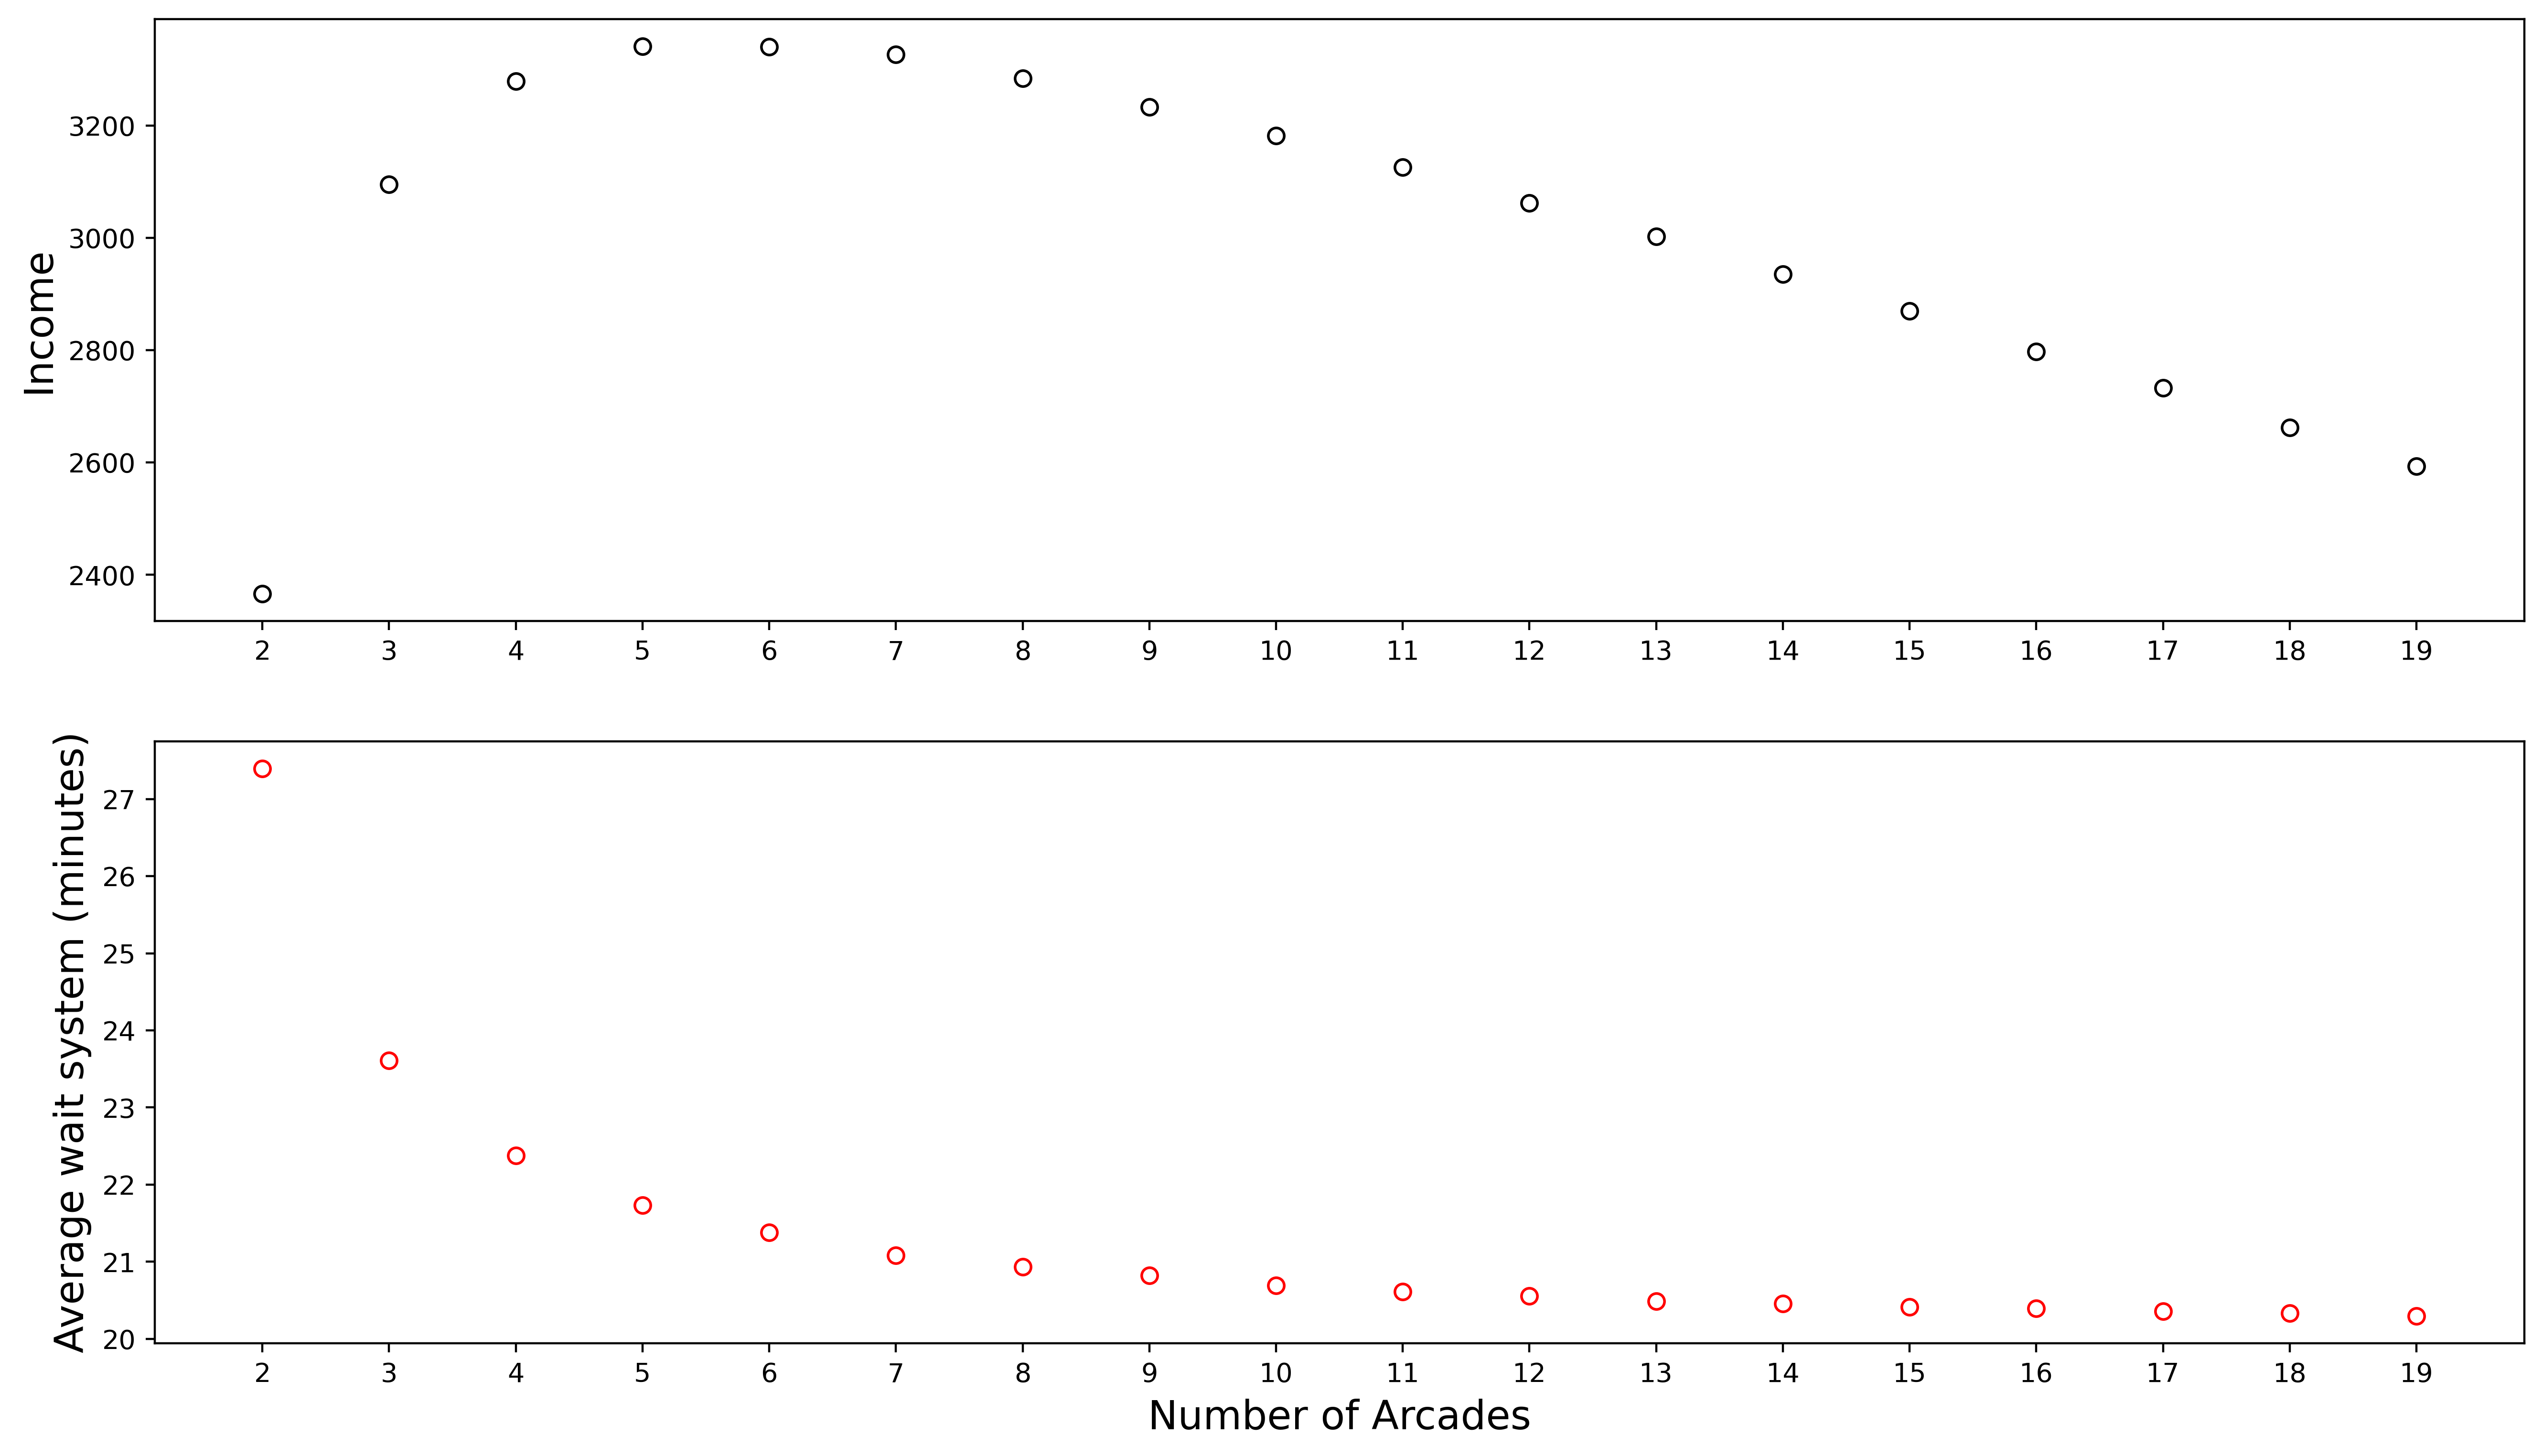
\includegraphics[scale=0.48]{images/avg_wait_sys_mor.png}
	\caption{Avg Wait System \& Income, 08:00-12:00 \& 17:00-22:00, $\lambda_{arrival}=\frac{1}{14} \frac{job}{min}$, b=256, k=64}\label{figura:avg_wait_sys_mor}
\end{figure}

Come si evince dal grafico, il numero ottimale di nodi Arcade per la prima e la terza fascia oraria, che permette di raggiungere entrambi gli obiettivi prefissati, è pari a 5.
\\ \\
Per quanto riguarda la seconda fascia oraria (12:00-17:00), è possibile osservare i risultati dell'analisi in figura \ref{figura:avg_wait_sys_aft}.
\begin{figure}[H]
	\centering
	\captionsetup{justification=centering,margin=2cm}
	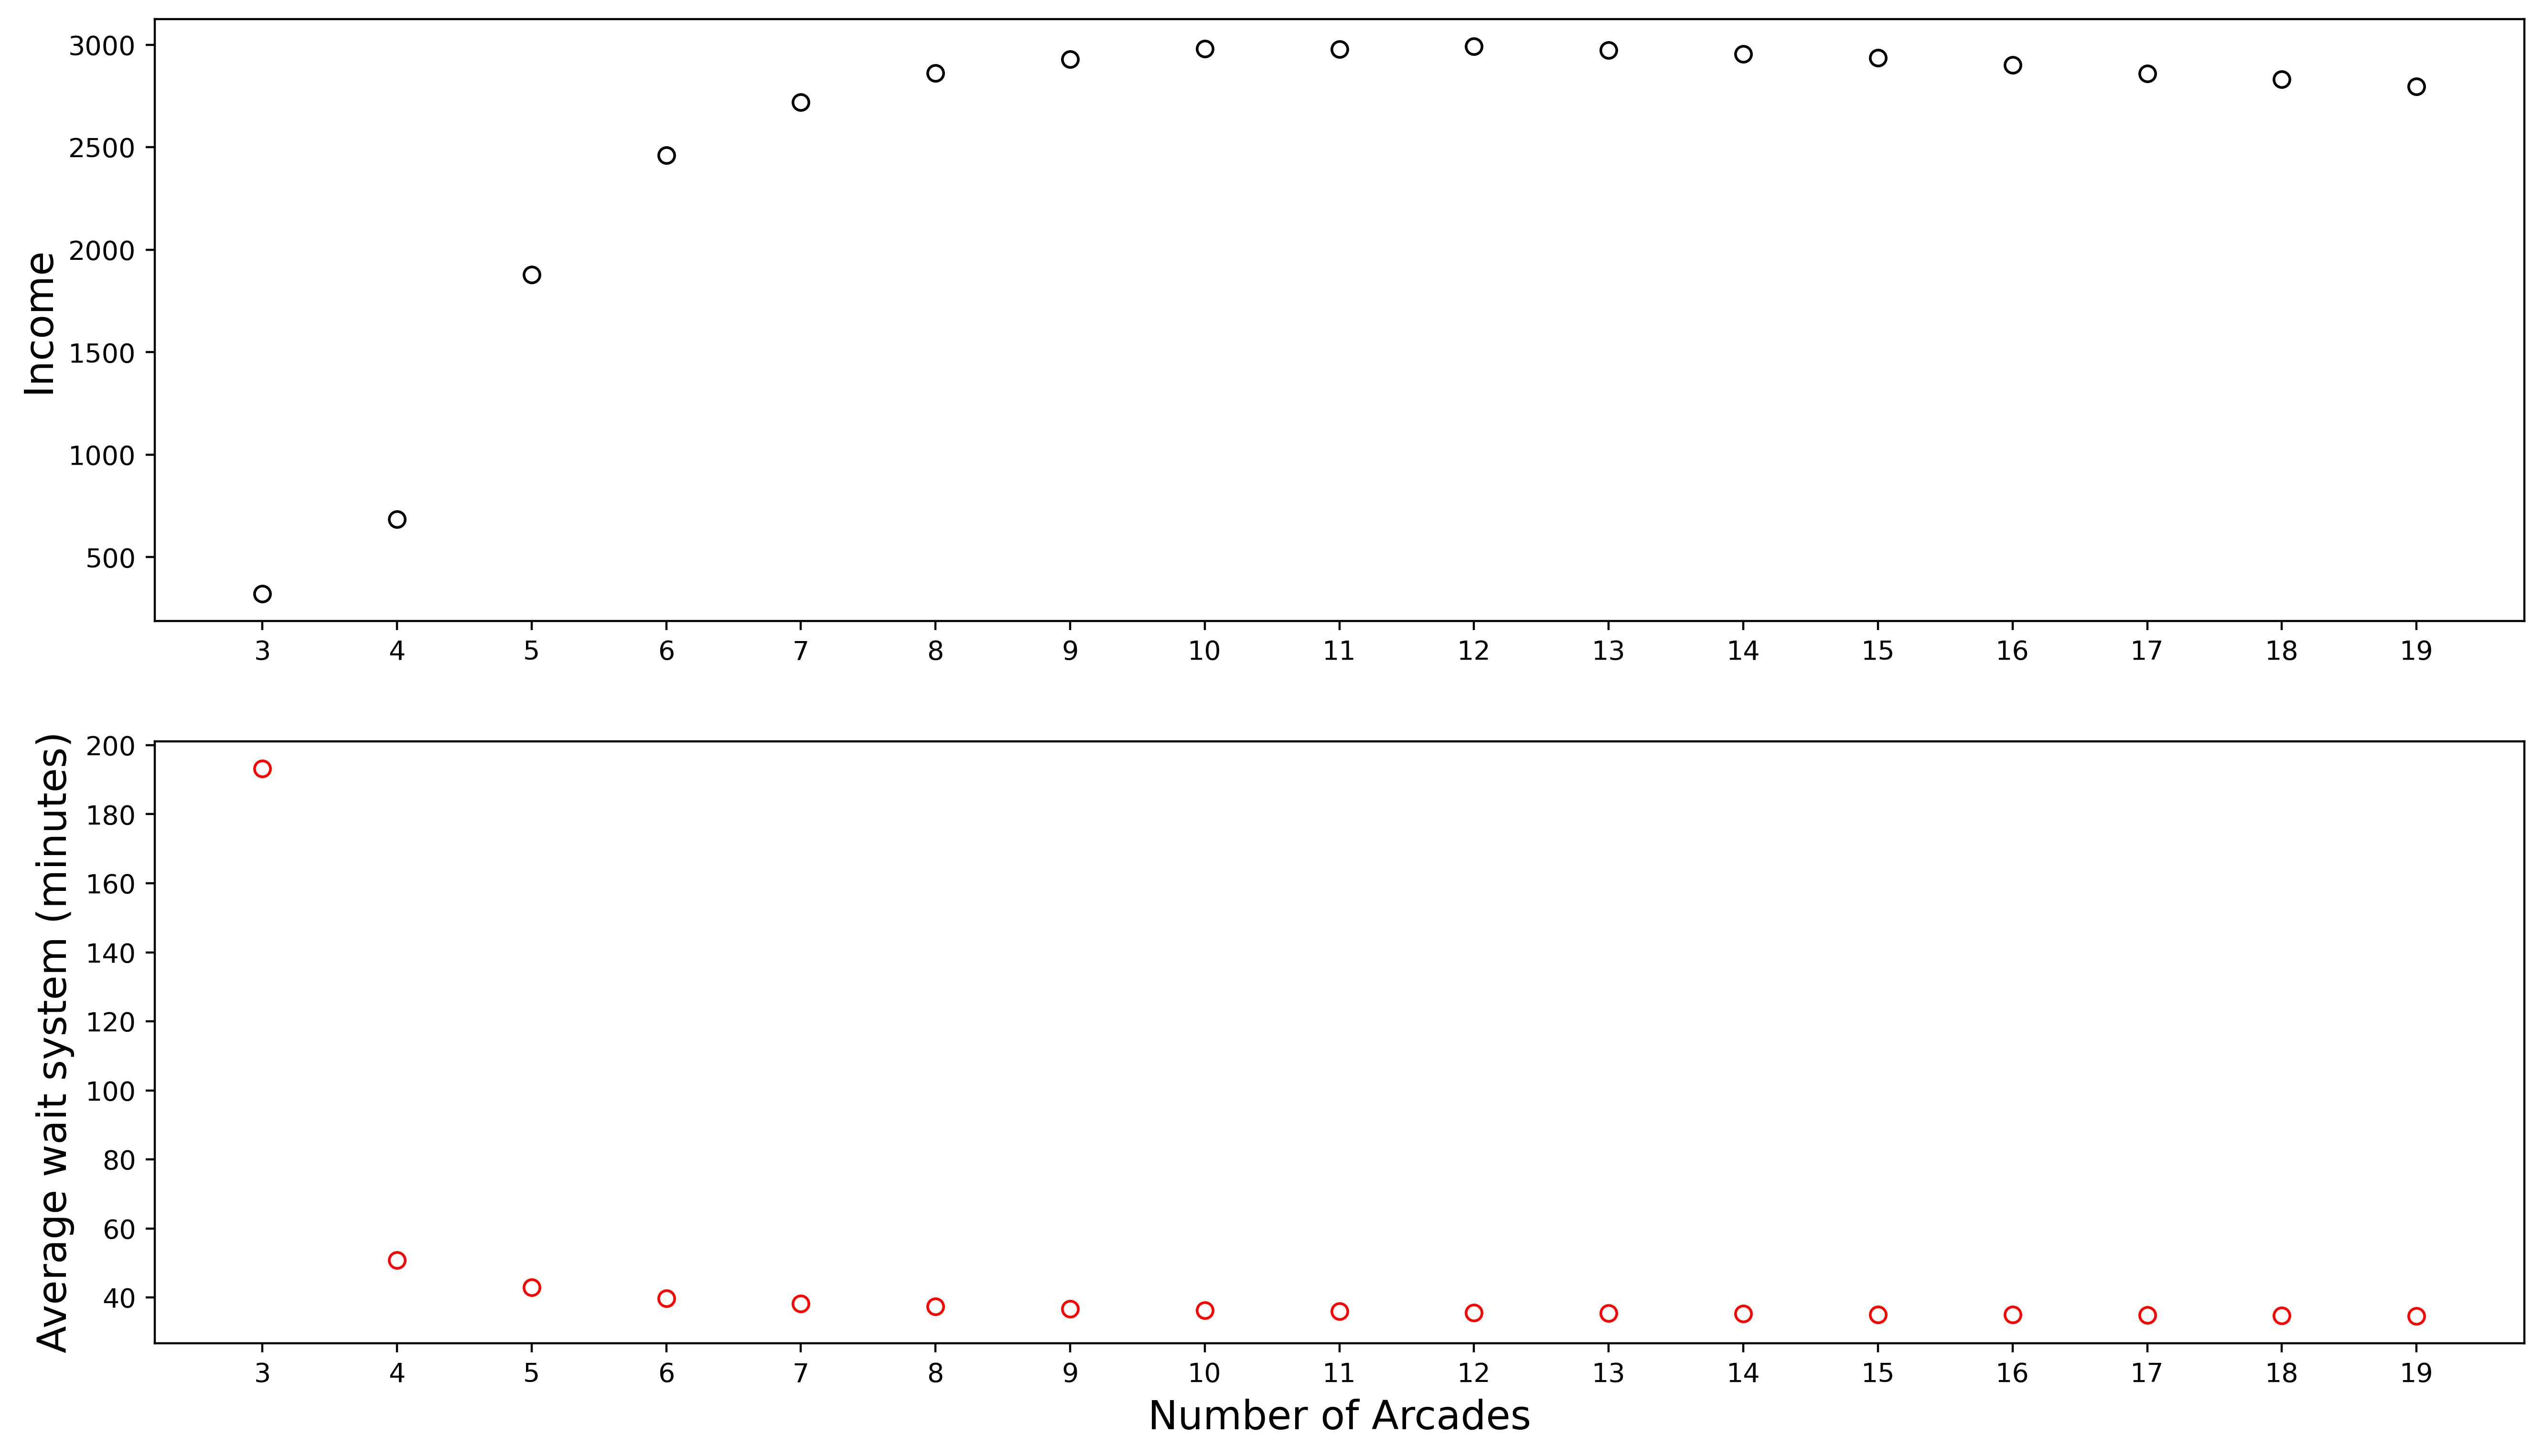
\includegraphics[scale=0.48]{images/avg_wait_sys_aft.png}
	\caption{Avg Wait System \& Income, 12:00-17:00, $\lambda_{arrival}=\frac{1}{5} \frac{job}{min}$, b=256, k=64}\label{figura:avg_wait_sys_aft}
\end{figure}
Il numero ottimale di server Arcade, per la seconda fascia oraria, è pari a 12.
\\ \\
Per quanto riguarda la quarta fascia oraria (22:00-08:00), è possibile osservare i risultati dell'analisi in figura \ref{figura:avg_wait_sys_night}.
\begin{figure}[H]
	\centering
	\captionsetup{justification=centering,margin=2cm}
	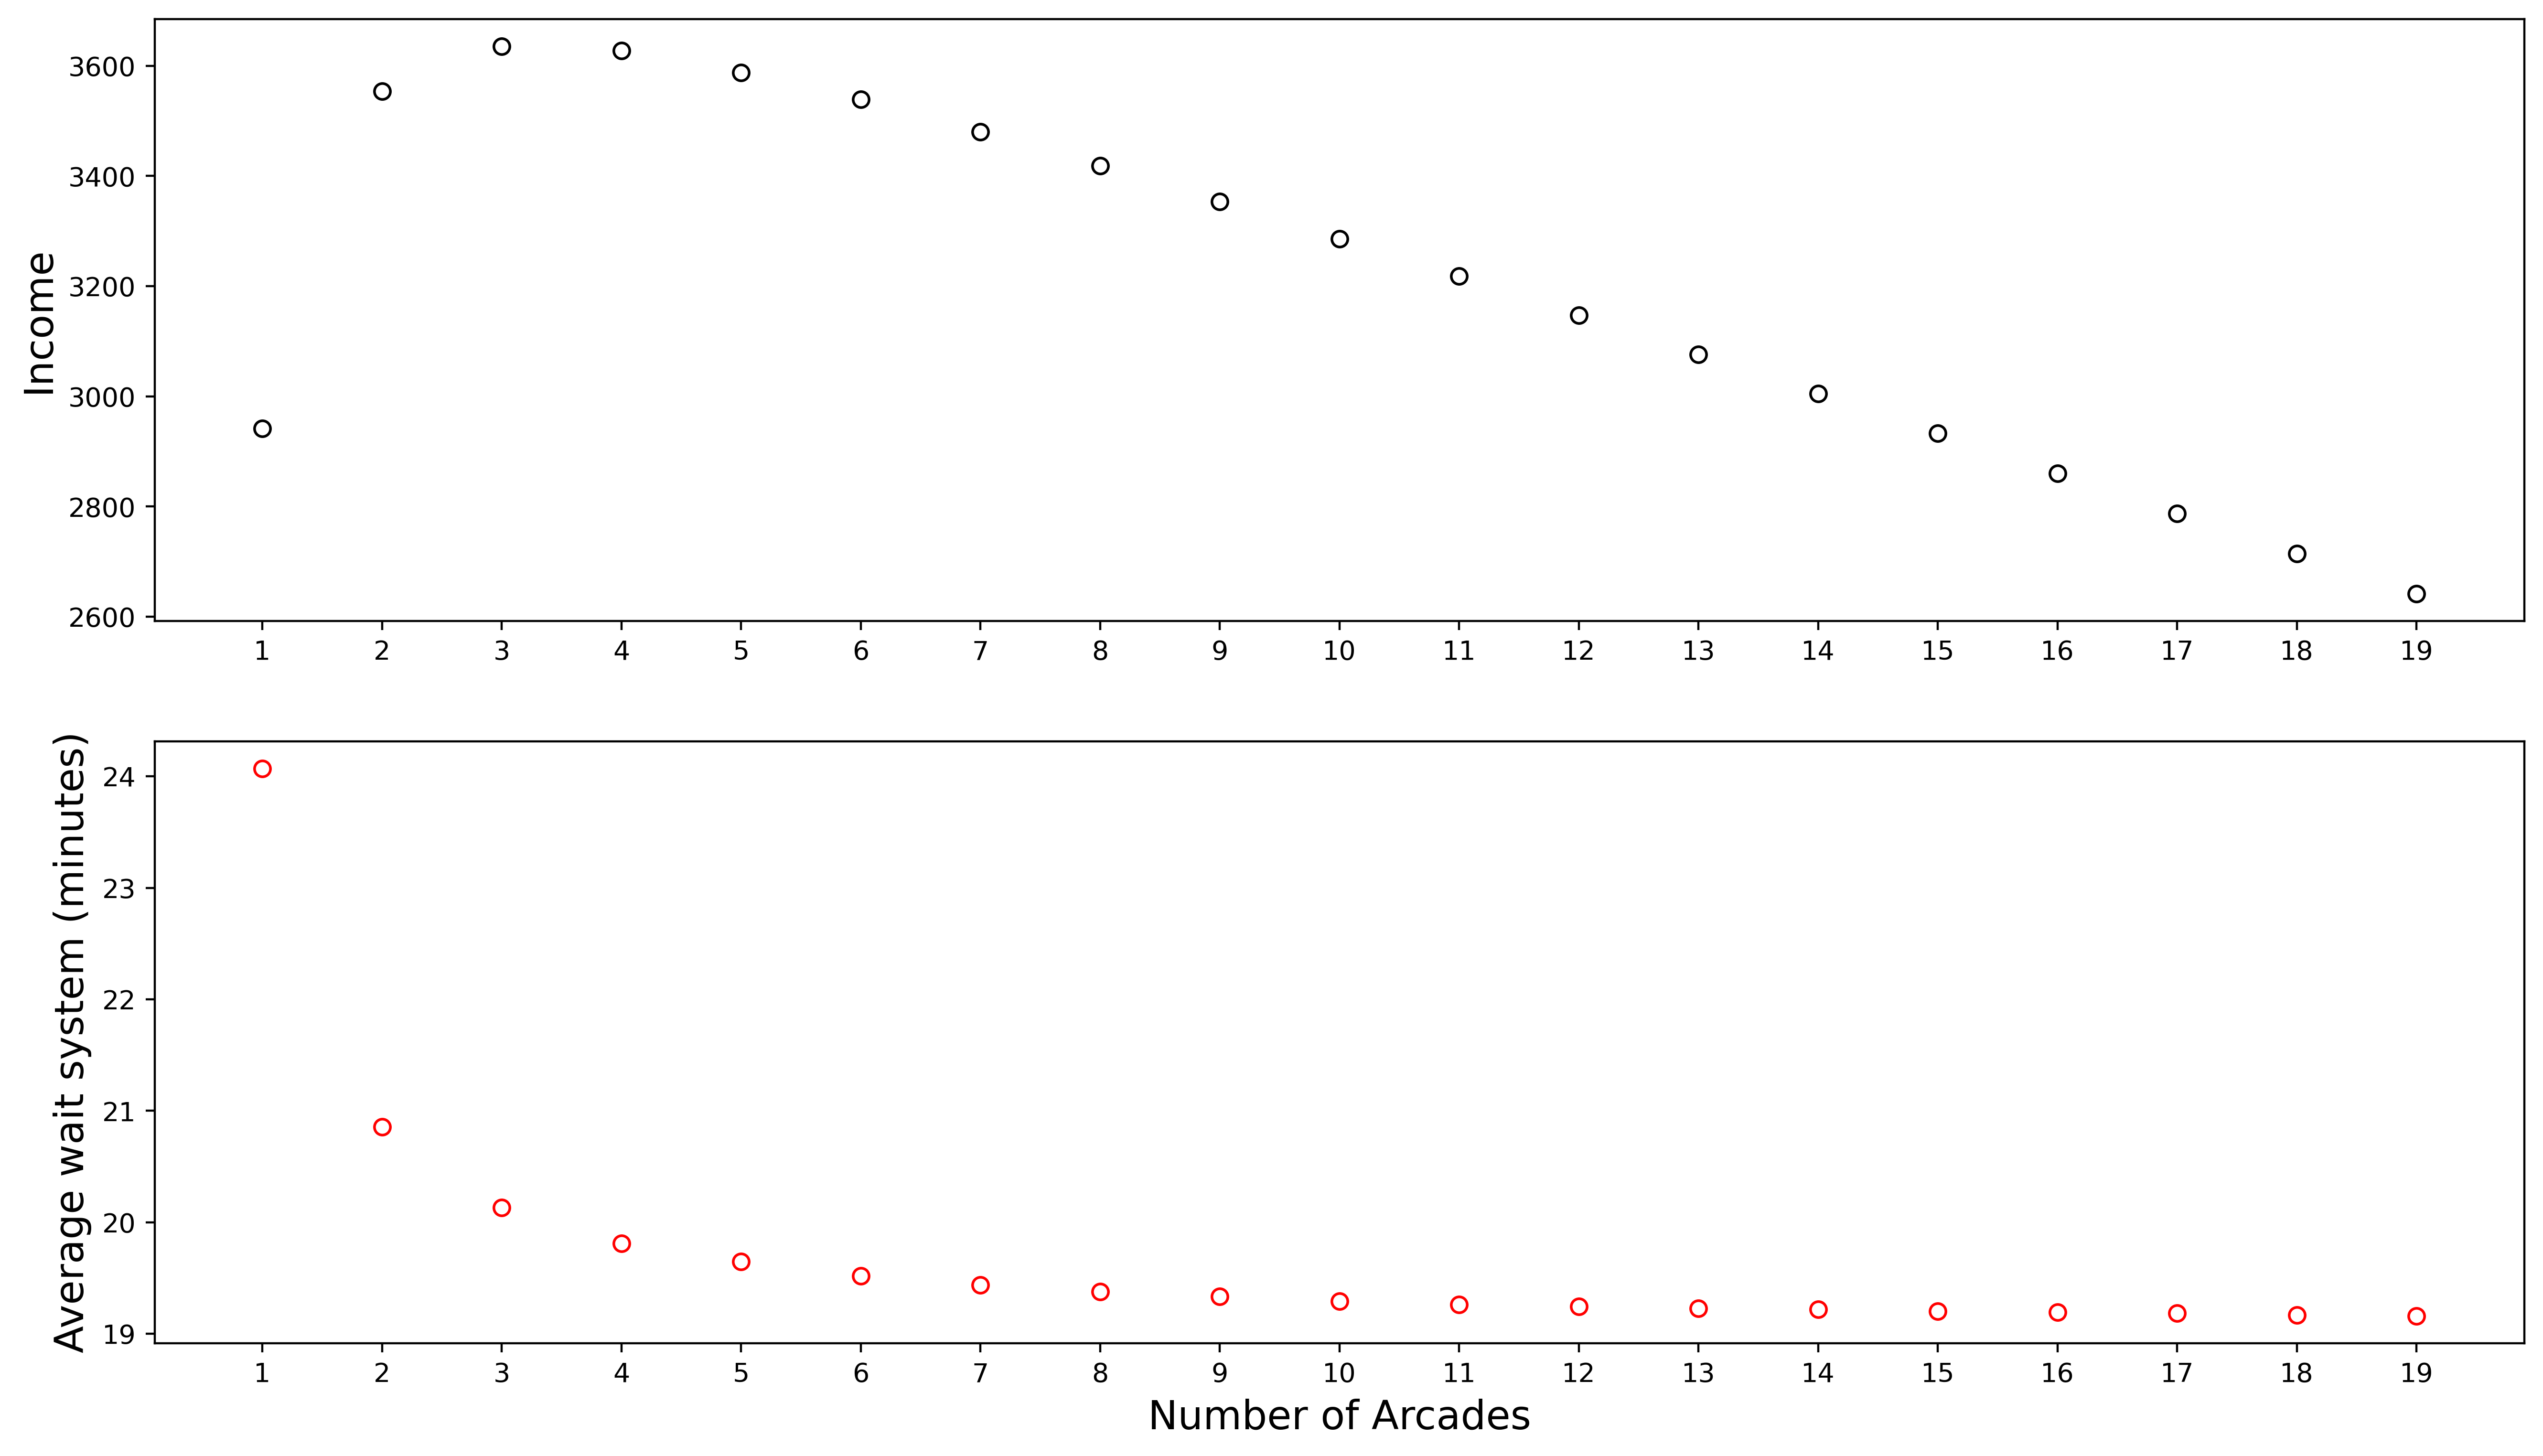
\includegraphics[scale=0.48]{images/avg_wait_sys_night.png}
	\caption{Avg Wait System \& Income, 22:00-08:00, $\lambda_{arrival}=\frac{1}{35} \frac{job}{min}$, b=256, k=64}\label{figura:avg_wait_sys_night}
\end{figure}
In questo caso, il numero ottimale di server Arcade da utilizzare è pari a 2.
\\ \\
In tabella \ref{tab3} è possibile individuare la configurazione ottimale dei nodi Arcade, per ogni fascia oraria.

\begin{table}[htbp]
\caption{Configurazione ottimale}
\begin{center}
\begin{tabular}{|c|c|}
\hline
\textbf{Fascia oraria} & \textbf{Configurazione ottimale $^{\mathrm{*}}$} \\ \hline
\textbf{08:00-12:00}  & 5 \\ \hline
\textbf{12:00-17:00}  & 12 \\ \hline
\textbf{17:00-22:00}  & 5 \\ \hline
\textbf{22:00-08:00} & 2 \\ \hline
\multicolumn{2}{l}{$^{\mathrm{*}}$ \textit{Numero di nodi Arcade nel sistema.}}
\end{tabular}
\label{tab3}
\end{center}
\end{table}
Sono stati effettuati run con seed diversi con la configurazione ottimale, precedentemente ricavata, per studiare il tempo di risposta medio, per ogni fascia oraria, con un intervallo di confidenza pari al $95\%$.

\begin{figure}[H]
	\centering
	\captionsetup{justification=centering,margin=2cm}
	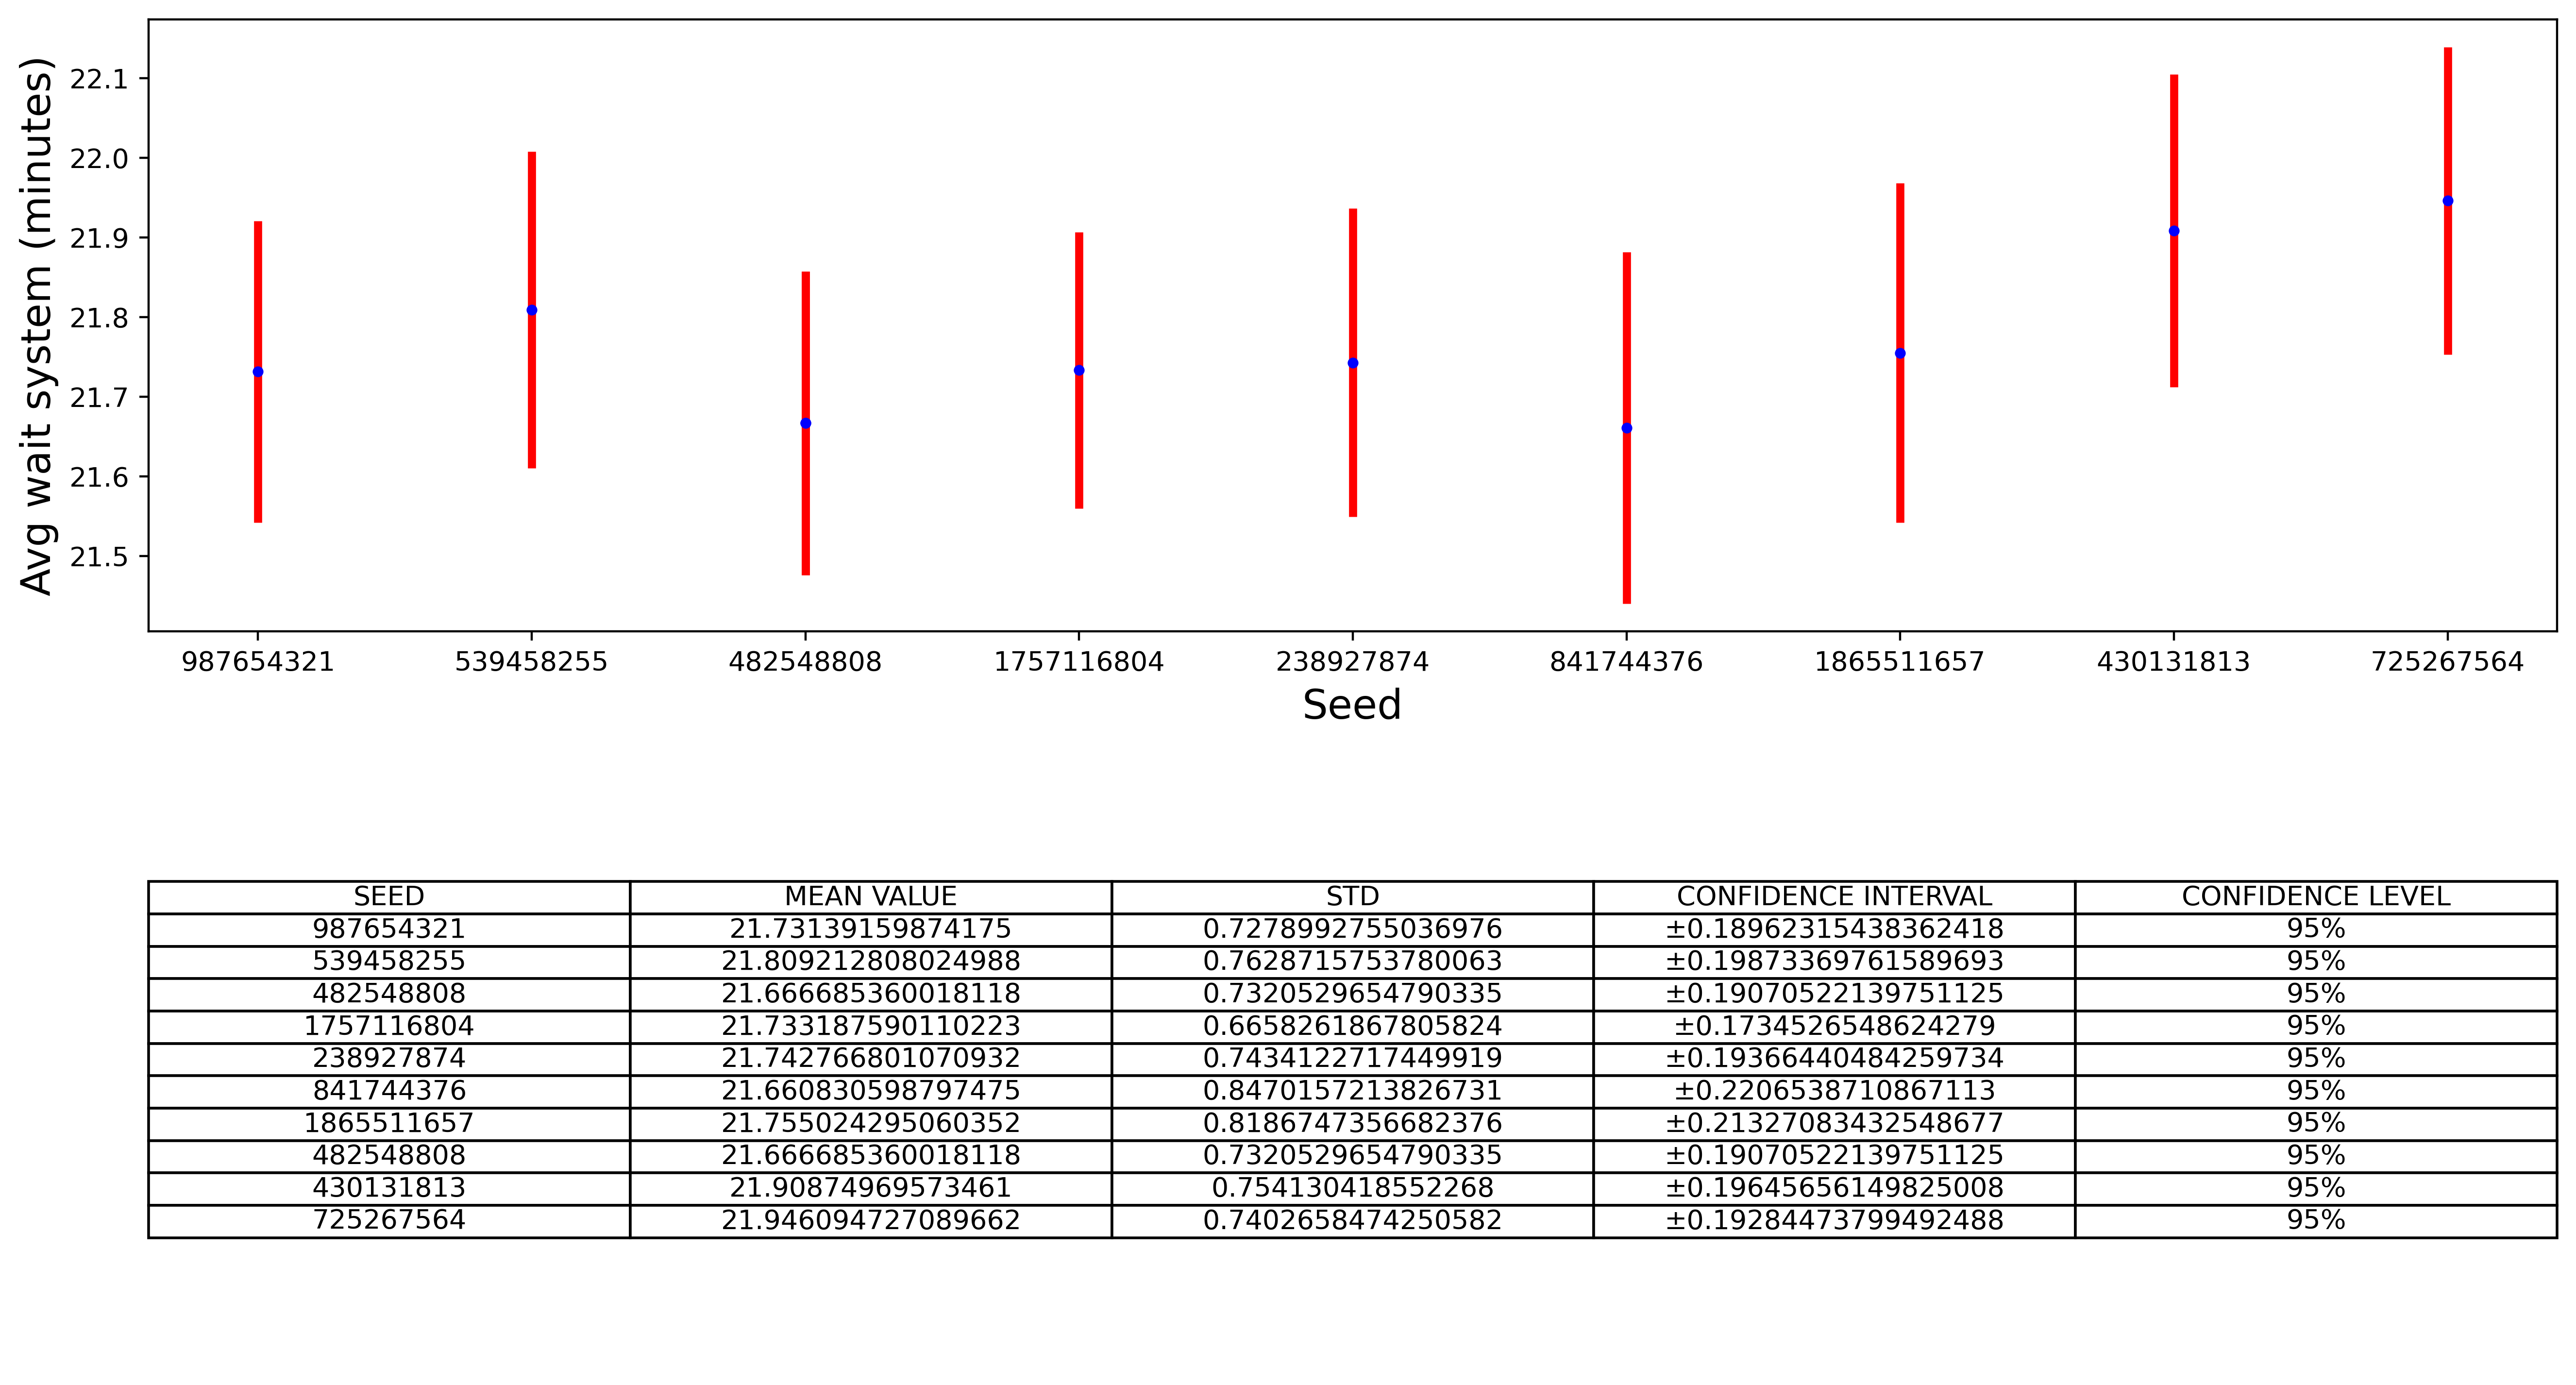
\includegraphics[scale=0.48]{images/avg_ws_steady_state_mor.png}
	\caption{Average Wait System, 08:00-12:00 \& 17:00-22:00, $\lambda_{arrival}=\frac{1}{14} \frac{job}{min}$, b=256, k=64}\label{figura:avg_ws_steady_state_mor}
\end{figure}

\begin{figure}[H]
	\centering
	\captionsetup{justification=centering,margin=2cm}
	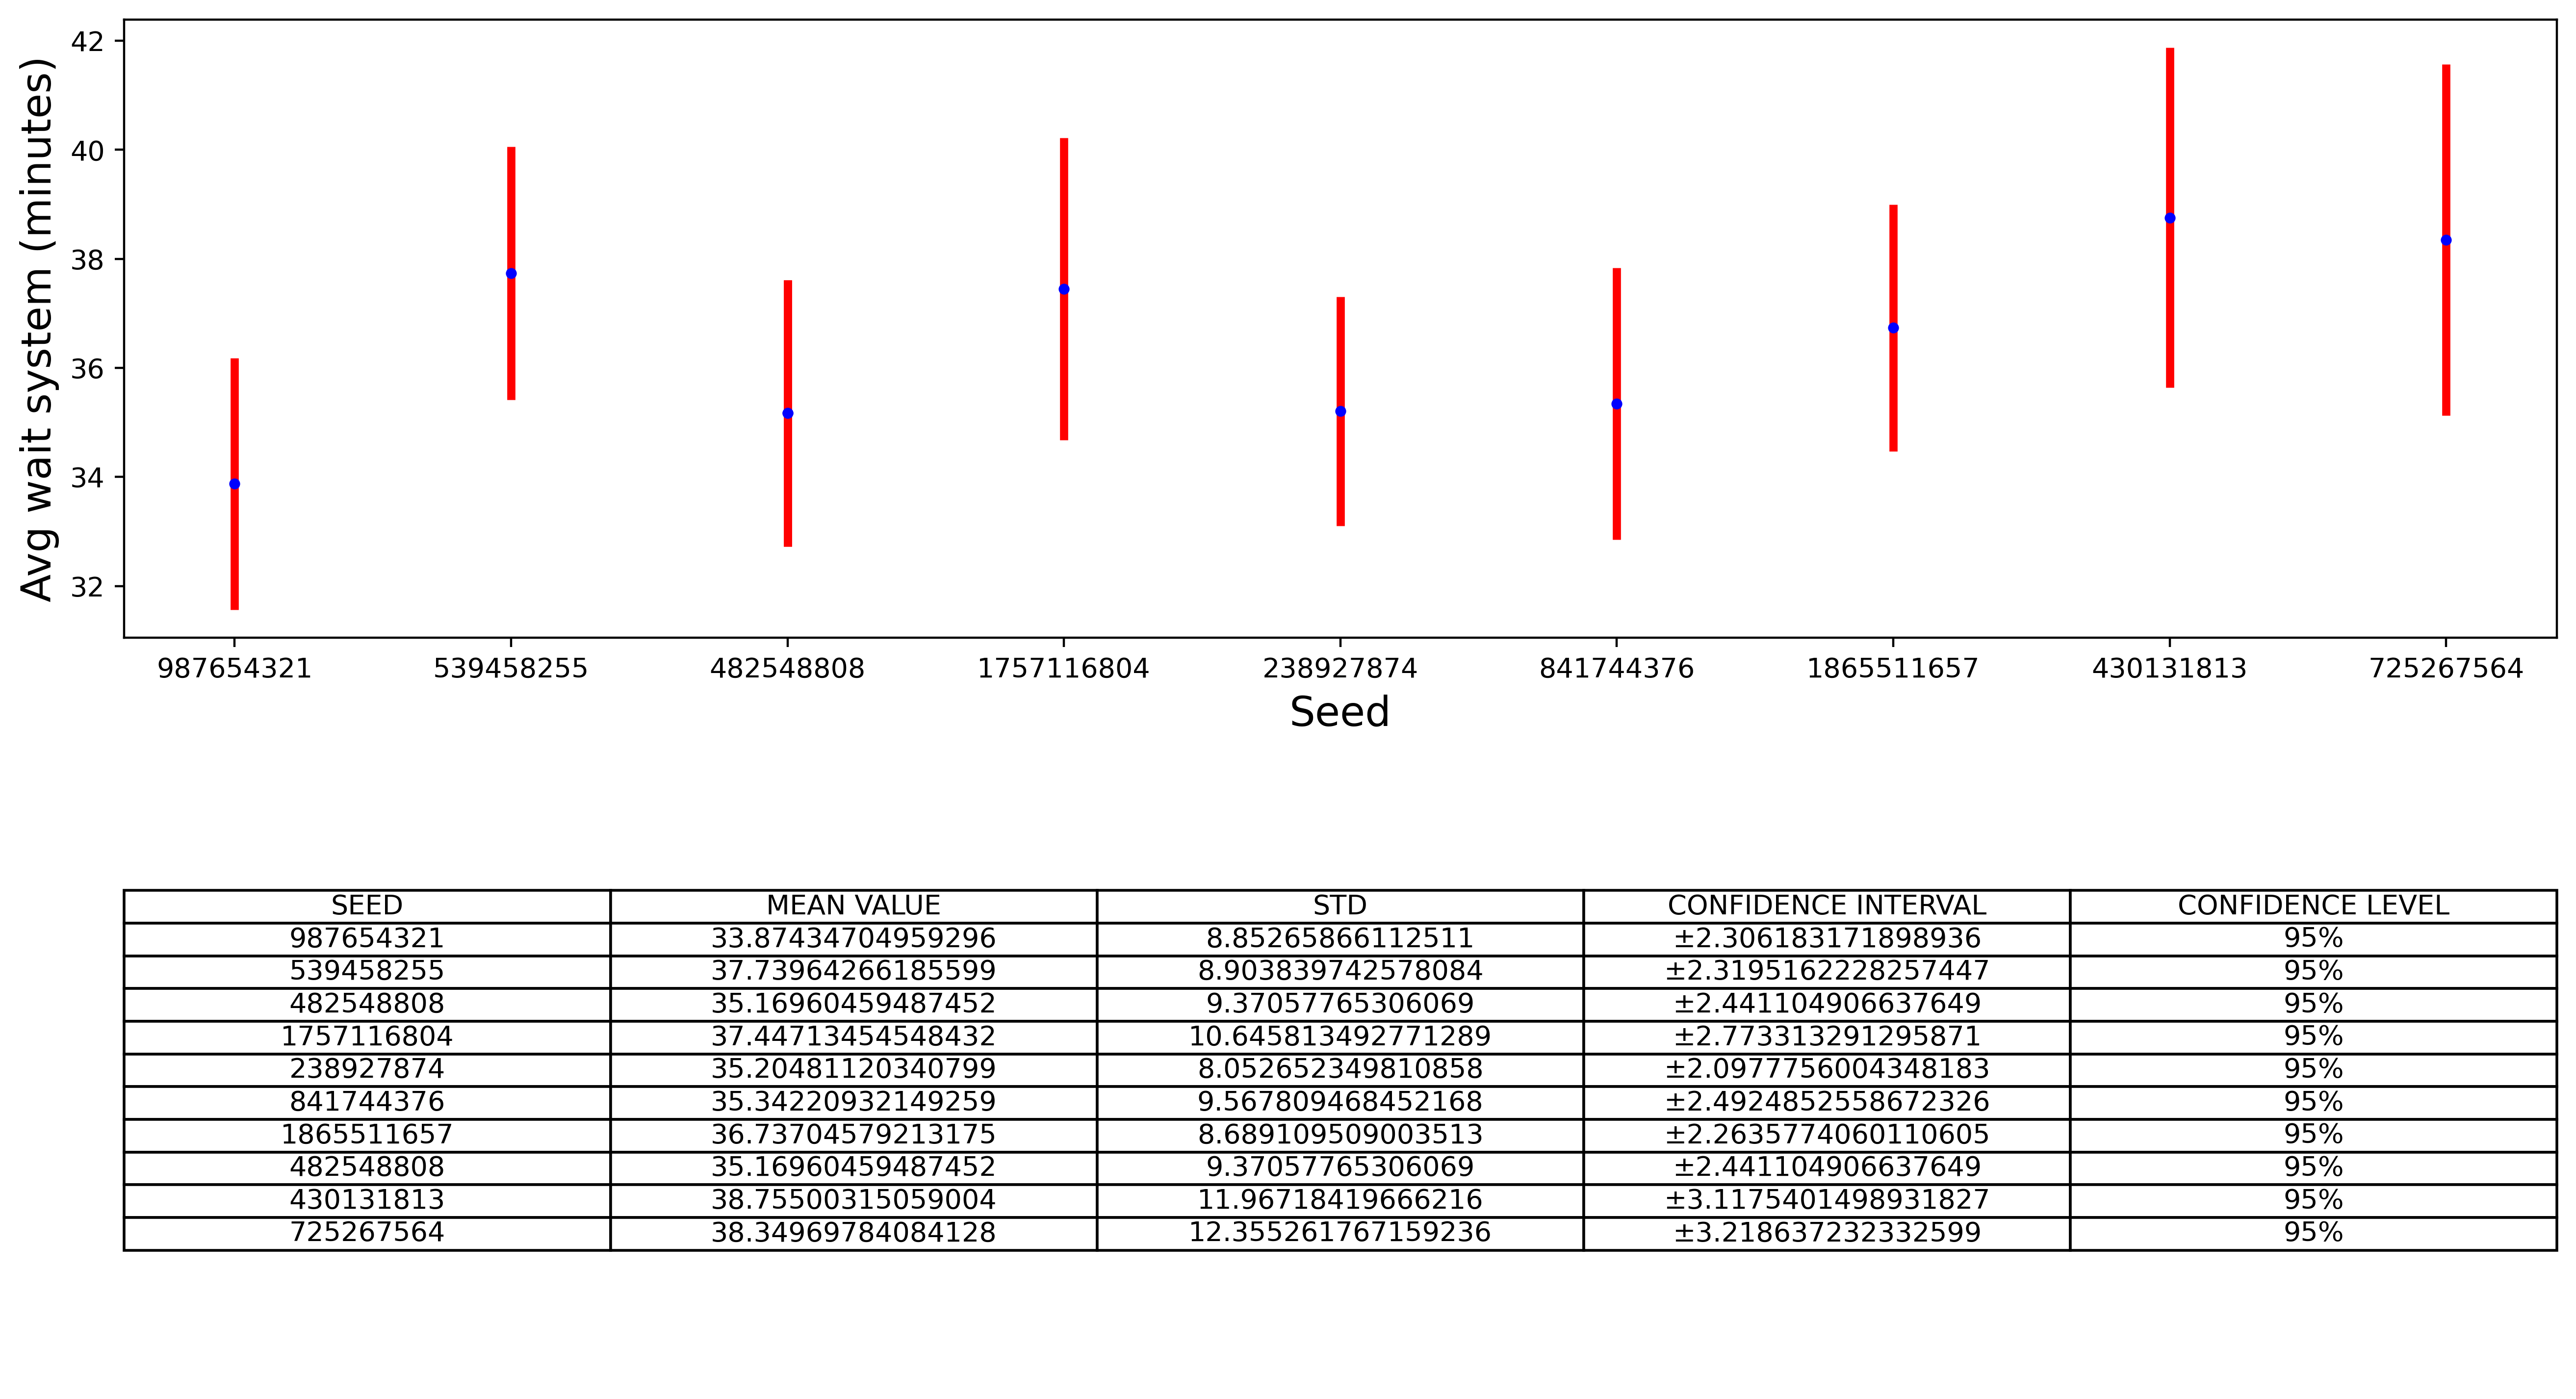
\includegraphics[scale=0.48]{images/avg_ws_steady_state_aft.png}
	\caption{Average Wait System, 12:00-17:00, $\lambda_{arrival}=\frac{1}{5} \frac{job}{min}$, b=256, k=64}\label{figura:avg_ws_steady_state_eve}
\end{figure}

\begin{figure}[H]
	\centering
	\captionsetup{justification=centering,margin=2cm}
	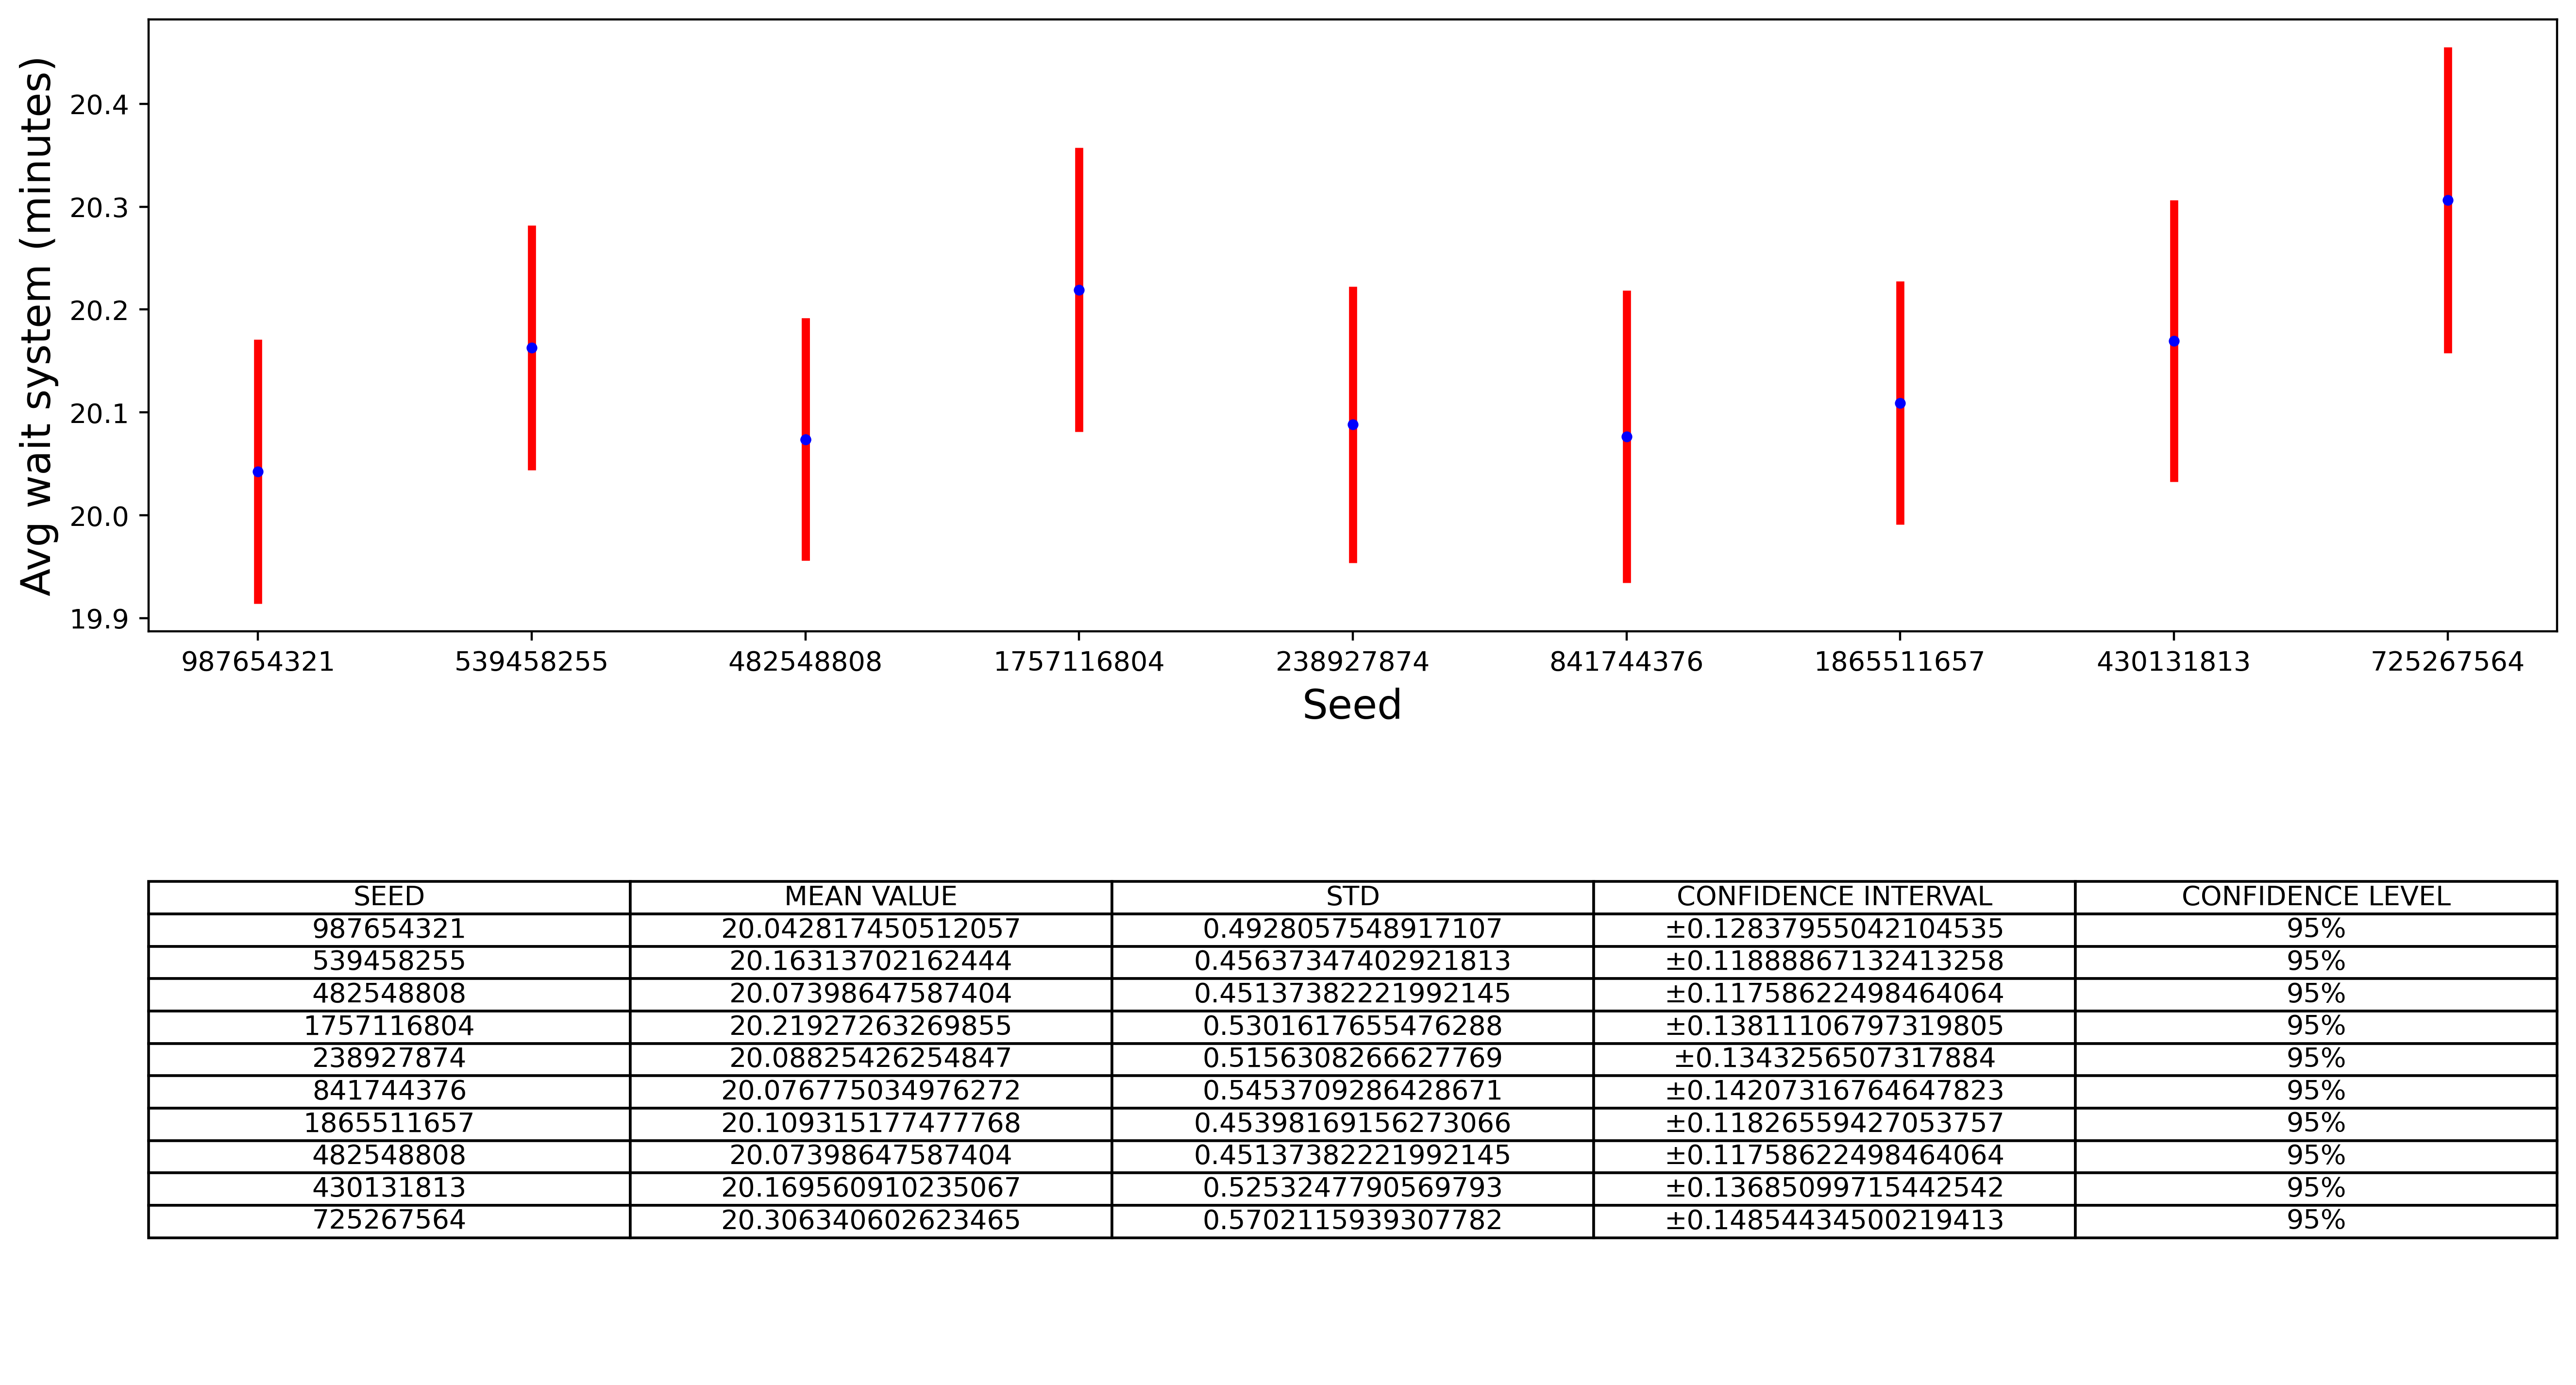
\includegraphics[scale=0.48]{images/avg_ws_steady_state_night.png}
	\caption{Average Wait System, 22:00-08:00, $\lambda_{arrival}=\frac{1}{35} \frac{job}{min}$, b=256, k=64}\label{figura:avg_ws_steady_state_night}
\end{figure}

\subsubsection{Analisi guadagno giornaliero}
Attraverso questa analisi viene effettuata una simulazione concreta di una tipica giornata lavorativa, con tre configurazioni differenti:
\begin{itemize}
	\item Configurazione minima (2 Arcade 08:00-12:00 \& 17:00-22:00, 3 Arcade 12:00-17:00, 1 Arcade 22:00-08:00);
	\item Configurazione ottimale(5 Arcade 08:00-12:00 \& 17:00-22:00, 12 Arcade 12:00-17:00, 2 Arcade 22:00-08:00);
	\item Configurazione massima(20 Arcade 08:00-12:00 \& 17:00-22:00, 20 Arcade 12:00-17:00, 20 Arcade 22:00-08:00).
\end{itemize} 
È possibile osservare il risultato di tale analisi in figura \ref{figura:ts_min}, \ref{figura:ts_optimal} e \ref{figura:ts_max}.
\begin{figure}[H]
	\centering
	\captionsetup{justification=centering,margin=2cm}
	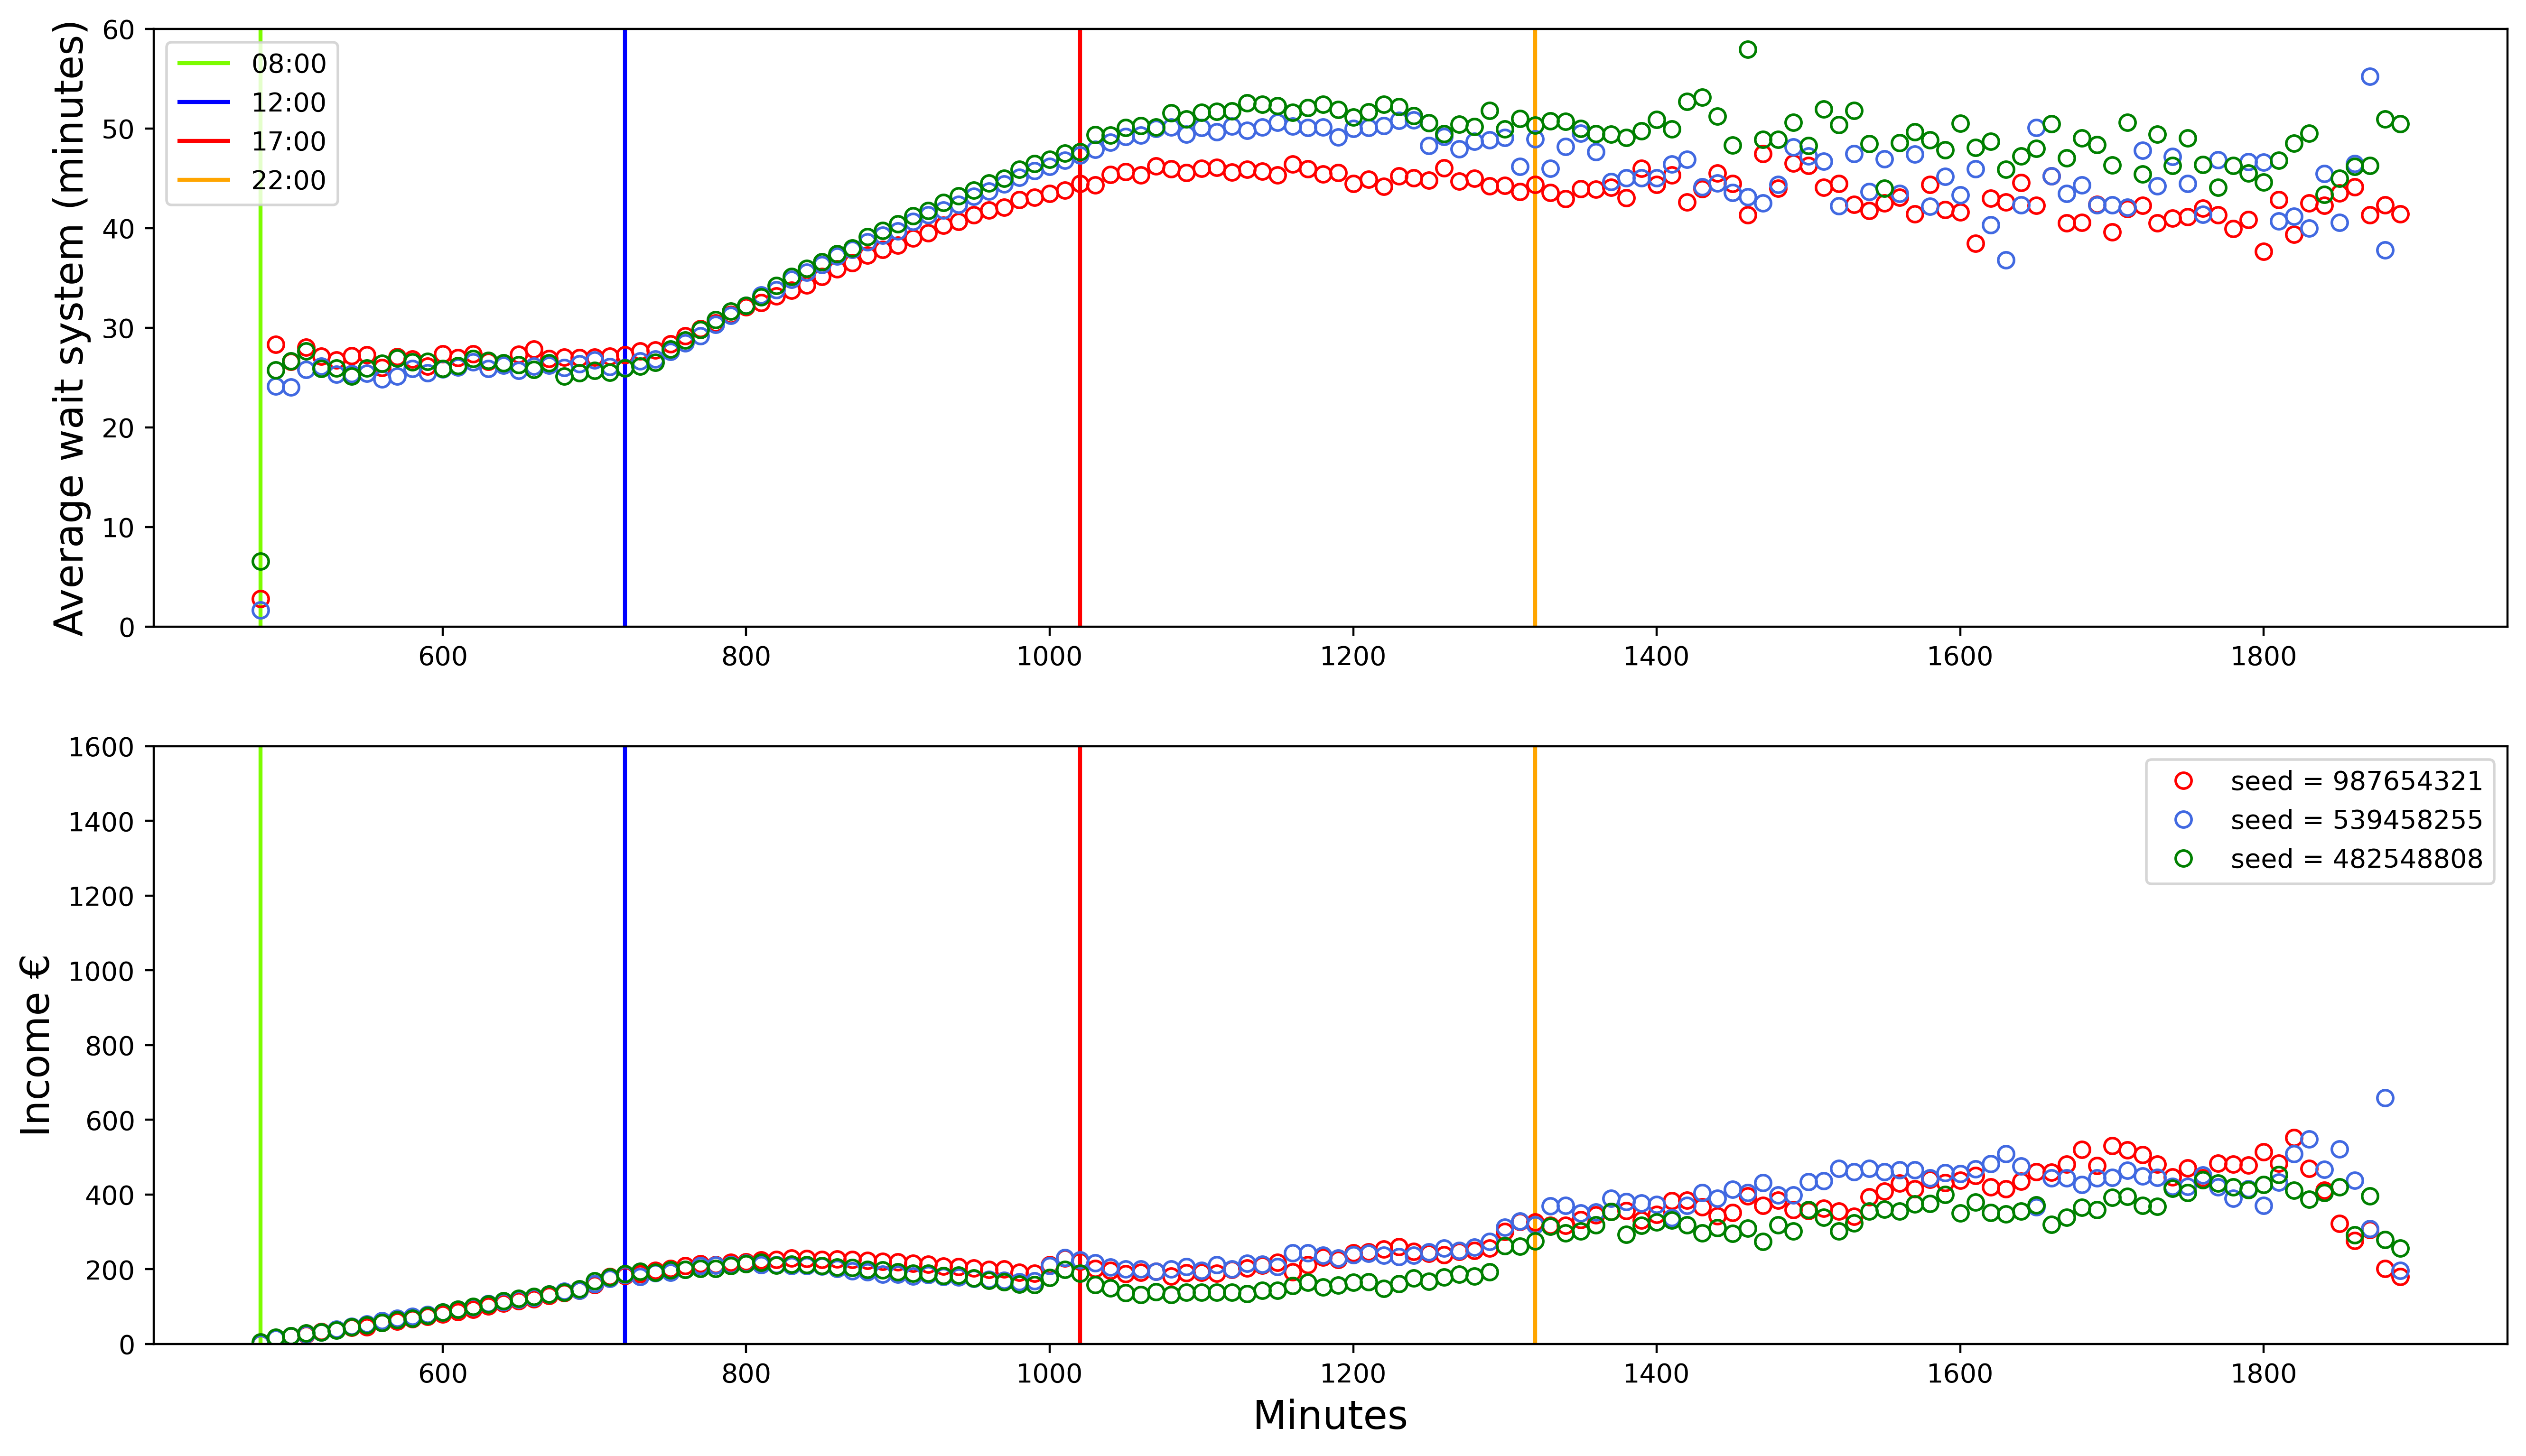
\includegraphics[scale=0.48]{images/ts_min.png}
	\caption{Average Wait System \& Income Daily, Base Model, minimal configuration, sampling frequency=10 min}\label{figura:ts_min}
\end{figure}
\begin{figure}[H]
	\centering
	\captionsetup{justification=centering,margin=2cm}
	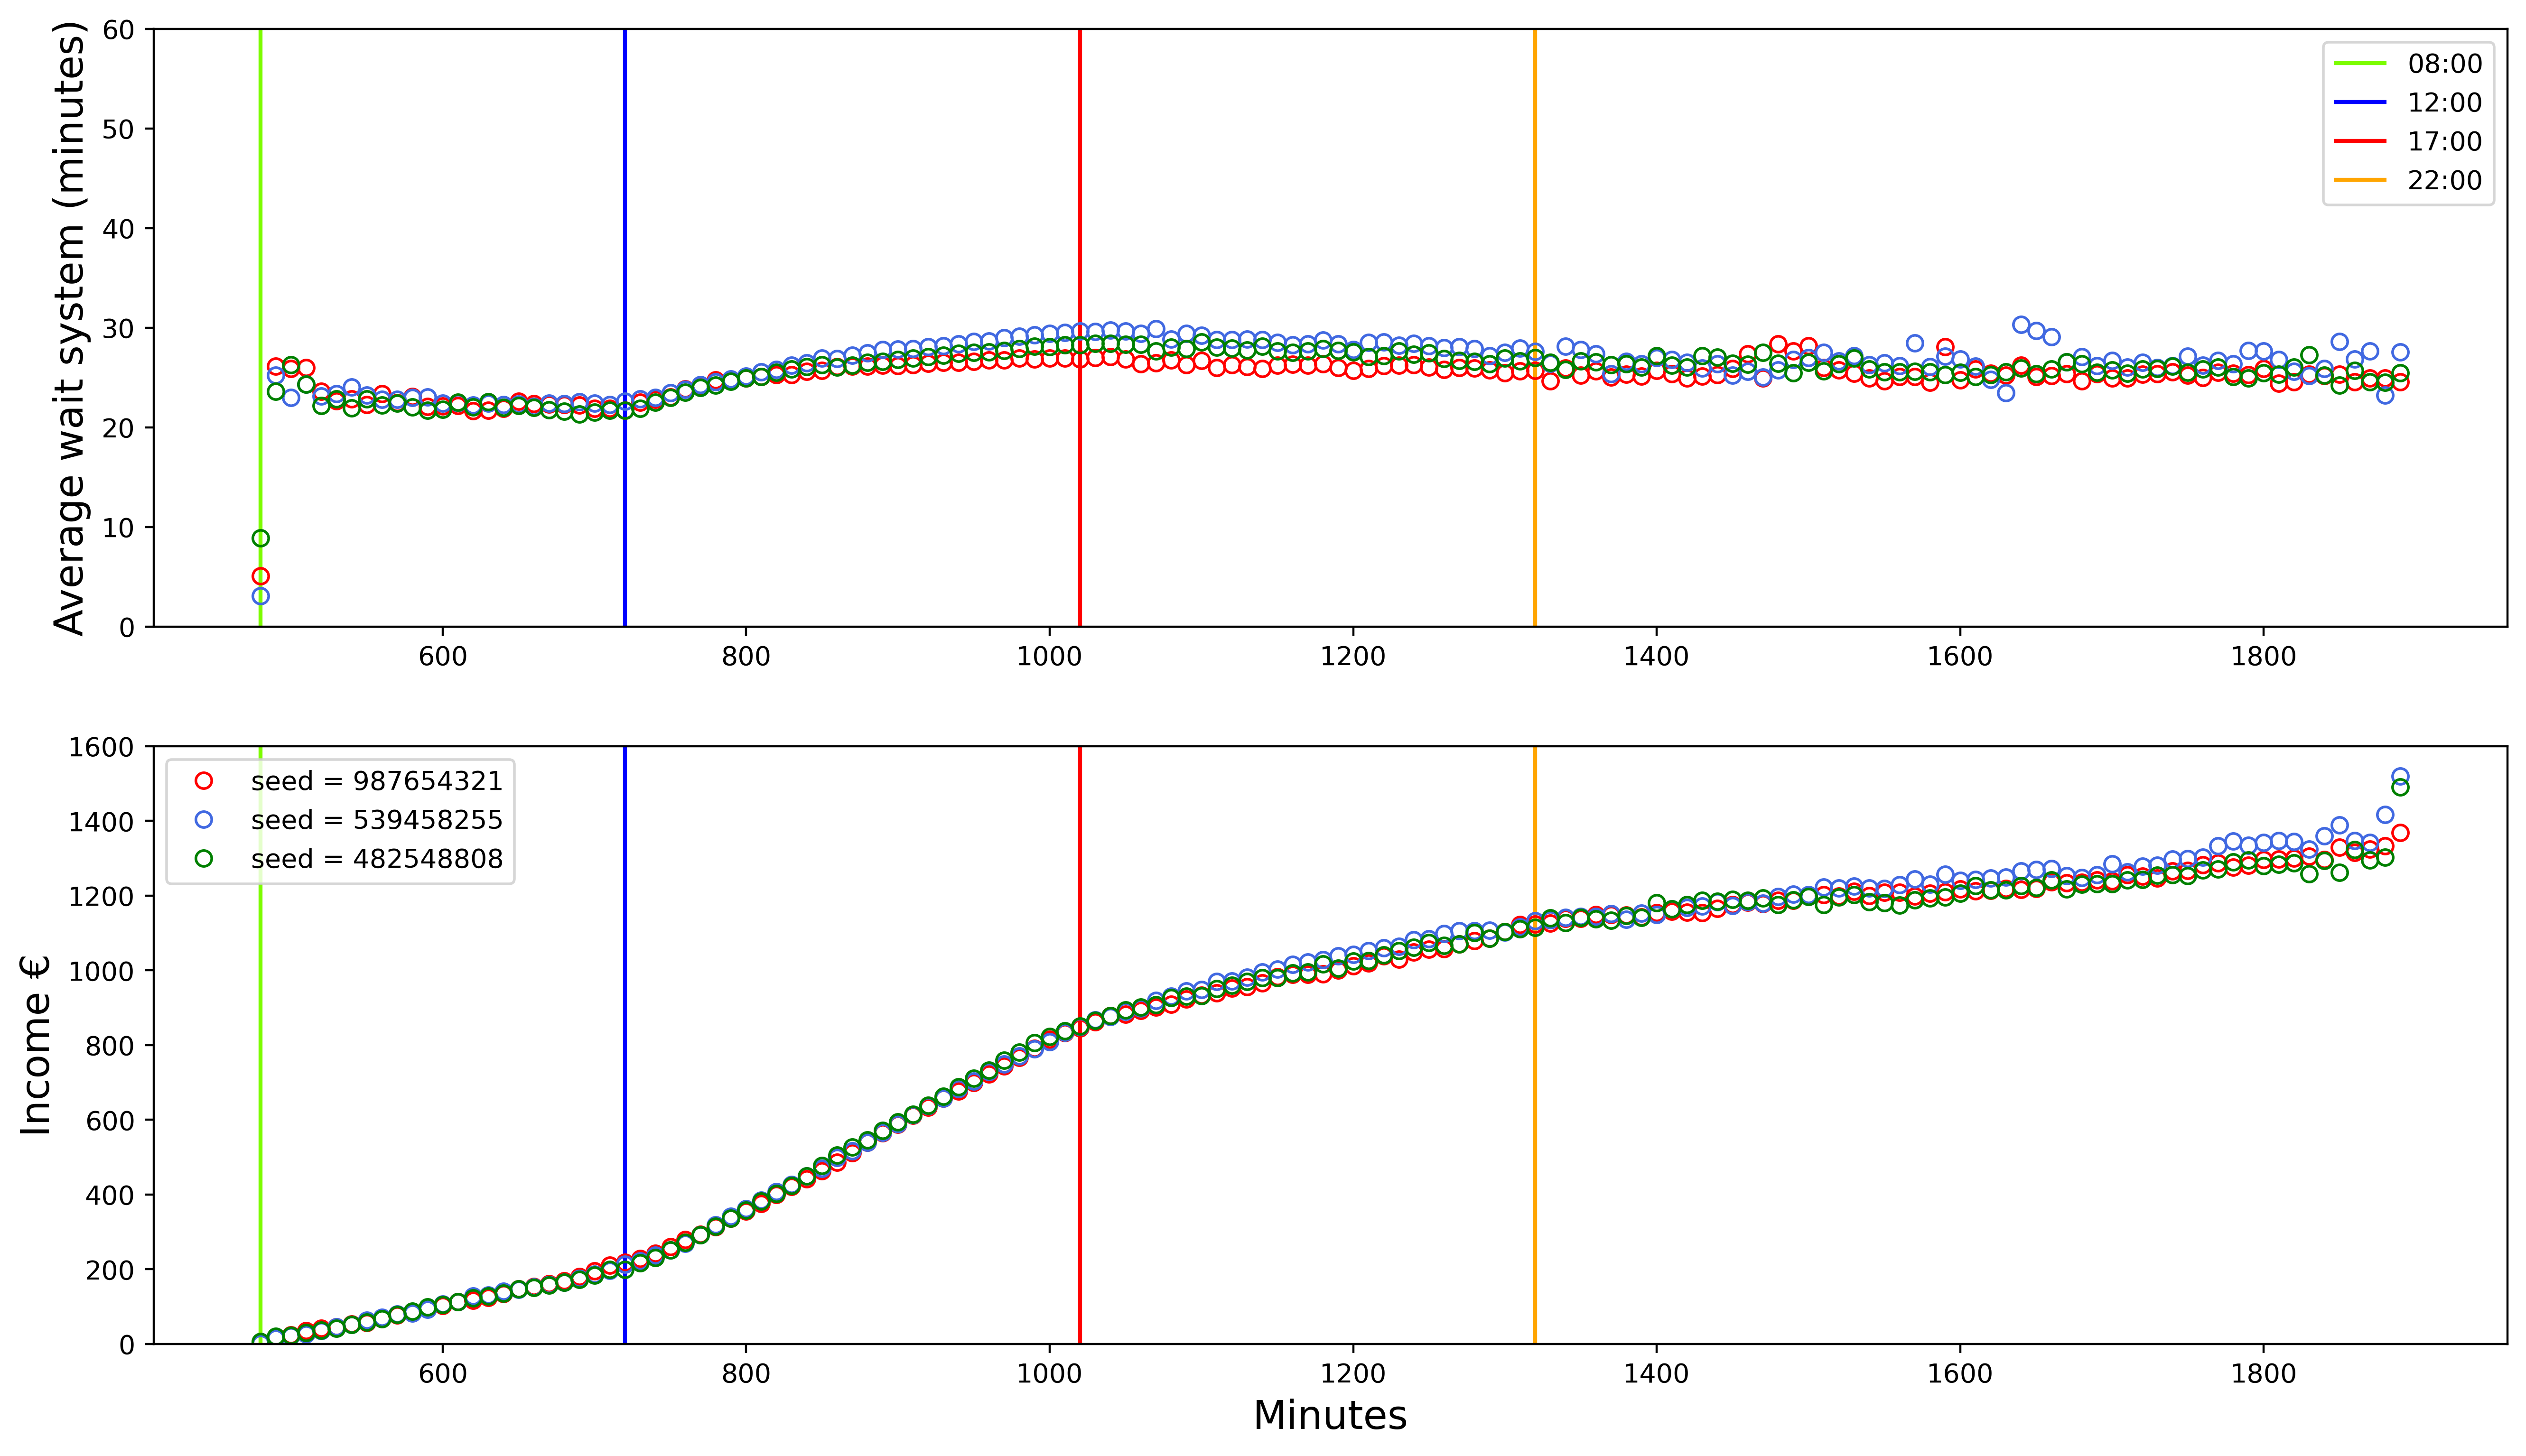
\includegraphics[scale=0.48]{images/ts_optimal.png}
	\caption{Average Wait System \& Income Daily, Base Model, best configuration, sampling frequency=10 min}\label{figura:ts_optimal}
\end{figure}
\begin{figure}[H]
	\centering
	\captionsetup{justification=centering,margin=2cm}
	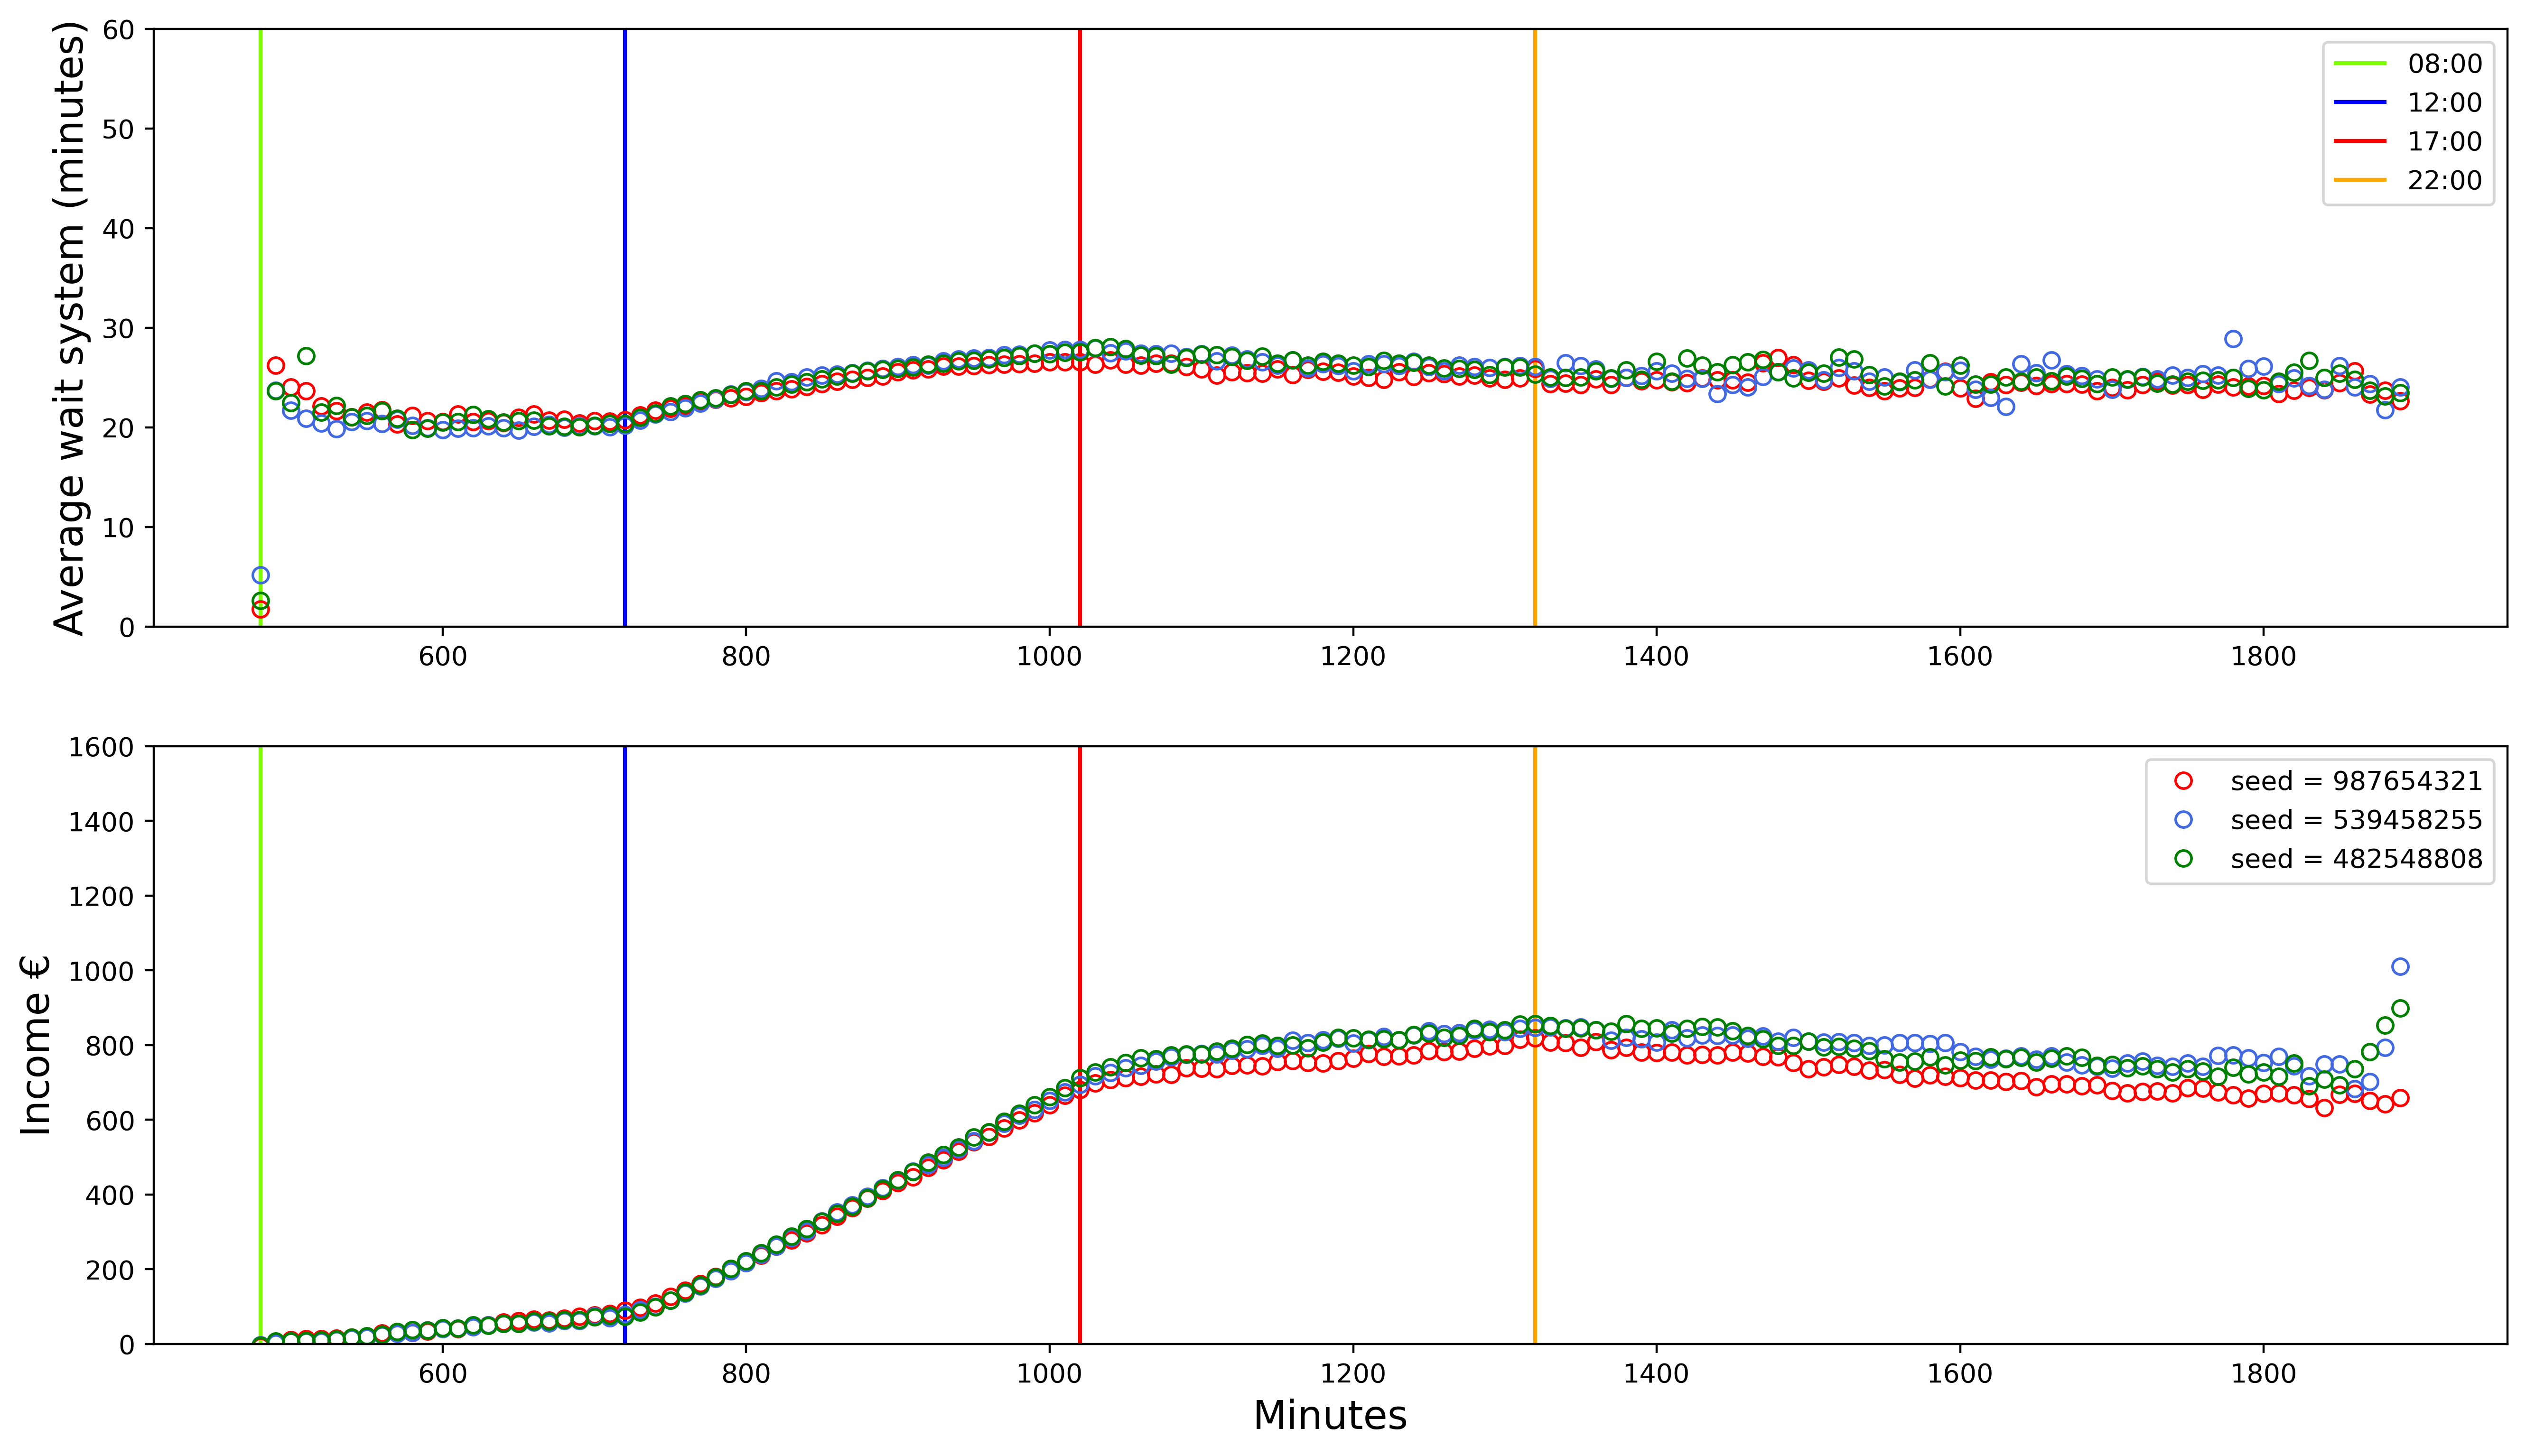
\includegraphics[scale=0.48]{images/ts_max.png}
	\caption{Average Wait System \& Income Daily, Base Model, maximum configuration, sampling frequency=10 min}\label{figura:ts_max}
\end{figure}
Come si evince da tali risultati, oltre a rispettare i QoS imposti, la configurazione ottimale porta ad un guadagno giornaliero migliore. Inoltre, si può osservare come il tempo di risposta medio del sistema della configurazione massimale è comparabile con quello della configurazione ottimale, nonostante quest'ultimo abbia un numero minore di nodi Arcade.

\section{Modello Avanzato} % Numbered section

Si procede alla realizzazione di un modello avanzato che sia in grado di adattarsi ai nuovi obiettivi, descritti in seguito, a costo zero. Per tale scopo, è stata introdotta nella sala giochi, la possibilità, da parte di un utente, di acquistare un biglietto \textit{premium} che gli permette di avere la precedenza rispetto agli utenti che sono in possesso di un biglietto standard.
\par In figura \ref{figura:adv_model_high_level} è possibile osservare lo schema ad alto livello del modello avanzato.
\begin{figure}[H]
	\centering
	\captionsetup{justification=centering,margin=2cm}
	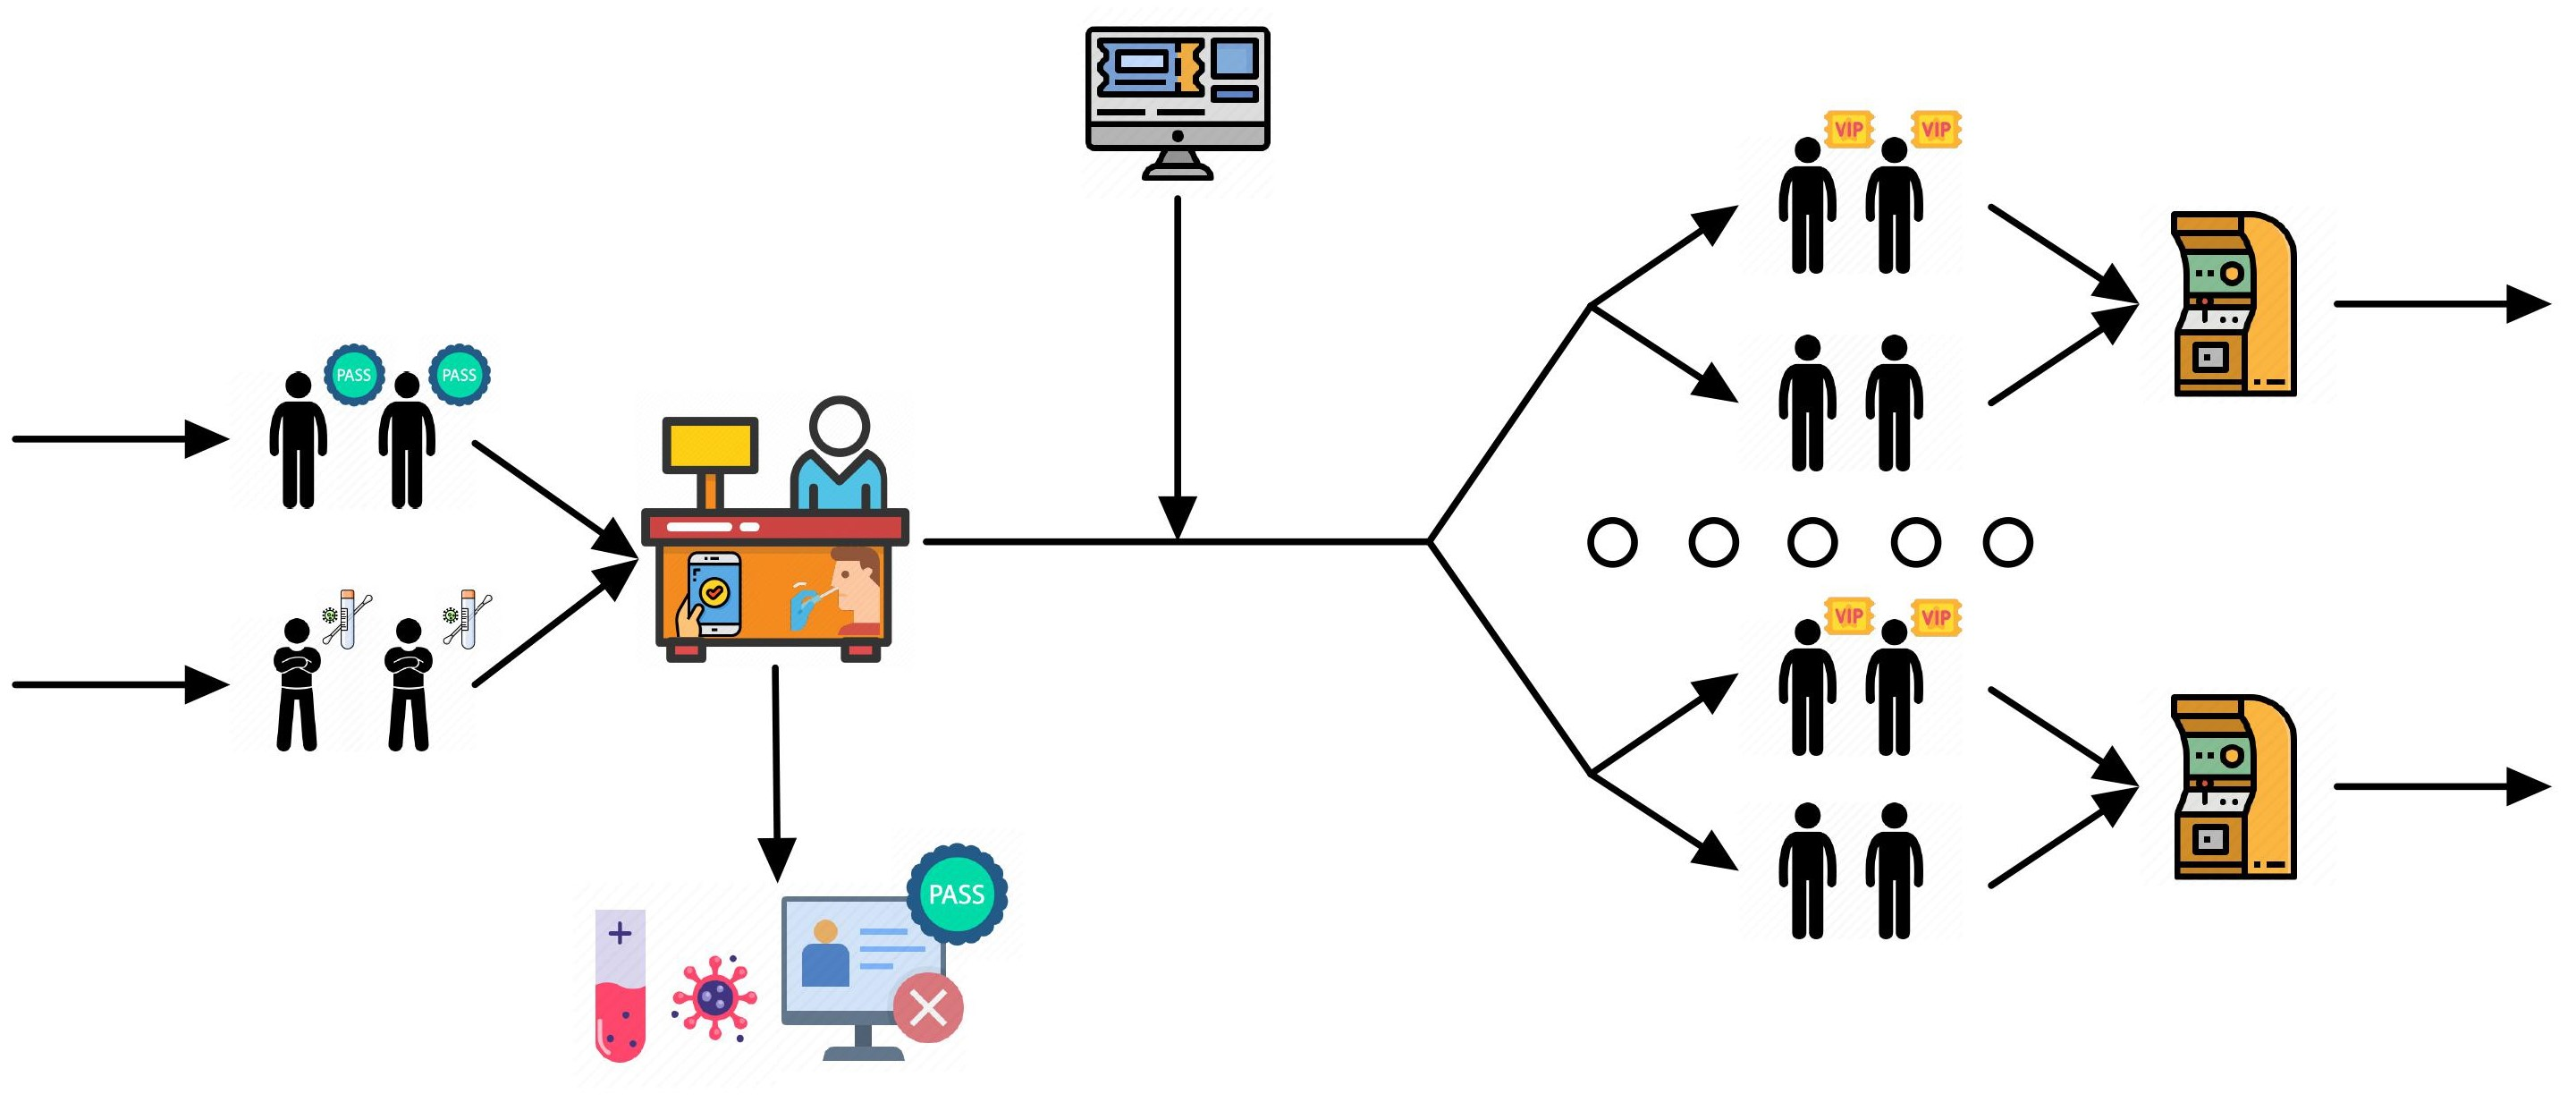
\includegraphics[scale=0.65]{images/adv_model_high_level.jpg}
	\caption{Advanced Model, High-level view}\label{figura:adv_model_high_level}
\end{figure}

\subsection{Obiettivi}
\label{Advanced_Goal}

\par Il primo obiettivo dello studio avanzato è quello di migliorare i profitti della sala giochi, rispetto al modello base. A tale scopo è stata definita una nuova funzione guadagno:

\begin{figure}[H]
	\centering
	\captionsetup{justification=centering,margin=2cm}
	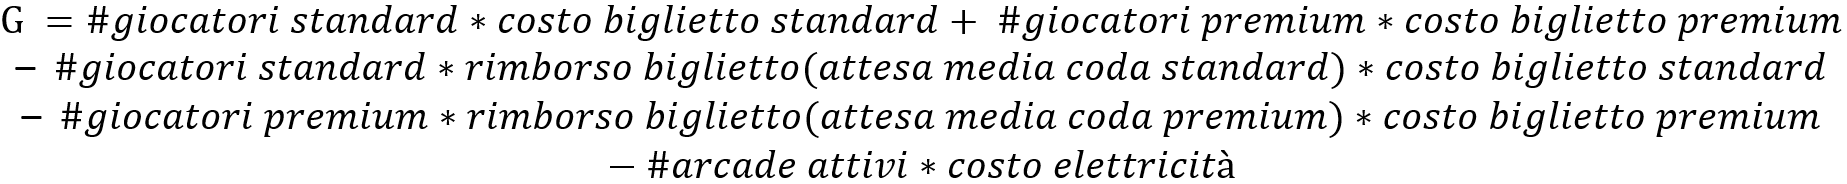
\includegraphics[scale=0.33]{images/adv_income.png}
	\label{figura:adv_income}
\end{figure}

Il costo del biglietto standard è di 10 \euro, mentre il costo del biglietto premium è di 20 \euro . Per quanto riguarda l'elettricità è stata considerata una spesa giornaliera per Arcade pari a $2.4 €$ \euro. La funzione \textit{rimborso biglietto}, che calcola la percentuale del \textit{costo biglietto} da restituire al giocatore, è proporzionale al tempo di attesa speso da quest'ultimo in coda nei nodi Arcade. La massima percentuale rimborsabile è del $80\%$. L'attesa minima in coda per cui è previsto il rimborso è di 8 minuti. 
\\
\par Il secondo obiettivo dello studio è quello di assicurare un tempo medio di attesa nella coda Covid-19, inferiore a quello del modello base, per gli utenti che possiedono il green-pass.

\subsection{Modello Concettuale}
Nel modello avanzato la sala giochi è modellata attraverso una rete aperta composta da N nodi rappresentanti i videogiochi (Arcade) e da un nodo rappresentante il controllo Covid-19. Ogni nodo Arcade si compone di un servente e di due code infinite con priorità astratta senza prelazione. L'accesso alla coda con priorità più alta è riservato agli utenti che acquistano il biglietto premium.
Il nodo Covid-19 si compone di un servente e di due code infinite con priorità size-based senza prelazione. L'accesso alla prima coda è riservato agli utenti che possiedono il green-pass, dato che questi ultimi hanno un tempo di servizio inferiore rispetto a chi esegue il test antigenico rapido.
\par Non sono state scelte code di priorità con prelazione, che avrebbero avuto prestazioni migliori per gli obiettivi prefissati, poiché non rispecchiano uno scenario reale.
\\
La struttura è aperta H24 e la giornata è suddivisa in 4 fasce orarie caratterizzate da tassi di arrivo differenti:
\begin{itemize}
\item 08:00-12:00
\item 12:00-17:00
\item 17:00-22:00
\item 22:00-08:00

\end{itemize}
Le variabili di stato del sistema considerate sono:
\begin{itemize}
\item Numero di clienti standard in ogni nodo;
\item Numero di clienti premium in ogni nodo;
\item Numero di nodi attivi;
\item Tipologia di cliente.
\end{itemize}
Le code inizialmente vengono considerate vuote, conseguentemente il numero di
clienti ad ogni nodo è 0. La tipologia di ogni cliente (Green-pass, tampone o biglietto online) è decisa aleatoriamente al suo arrivo. I nodi per ogni fase vengono definiti aperti o chiusi in base alla configurazione scelta durante lo studio.
\\ \\
Gli eventi considerati sono:
\begin{itemize}
\item Arrivo di un cliente standard;
\item Arrivo di un cliente premium;
\item Completamento di un servizio;
\item Cambio di fascia oraria.
\end{itemize}
Tali eventi possono causare cambiamenti dello stato. L’arrivo di un cliente causa l’aumento della popolazione in un dato nodo e nel sistema. Il completamento di un servizio causa il passaggio di un cliente da un
nodo ad un altro o la sua uscita dal sistema. Il cambio di fascia oraria può causare
l’accensione o lo spegnimento degli Arcade. Se un nodo arcade viene spento quando ha ancora un cliente in servizio, questo continuerà a processarlo, pur non ricevendo altri
arrivi, mentre i clienti in coda vengono distribuiti uniformemente tra i nodi Arcade rimasti operativi. Il tempo in cui un nodo Arcade è idle, ma acceso, viene considerato nel calcolo dei
costi.

\par In figura \ref{figura:adv_model_low_level} è possibile osservare lo schema a basso livello del modello avanzato. 

\begin{figure}[H]
	\centering
	\captionsetup{justification=centering,margin=2cm}
	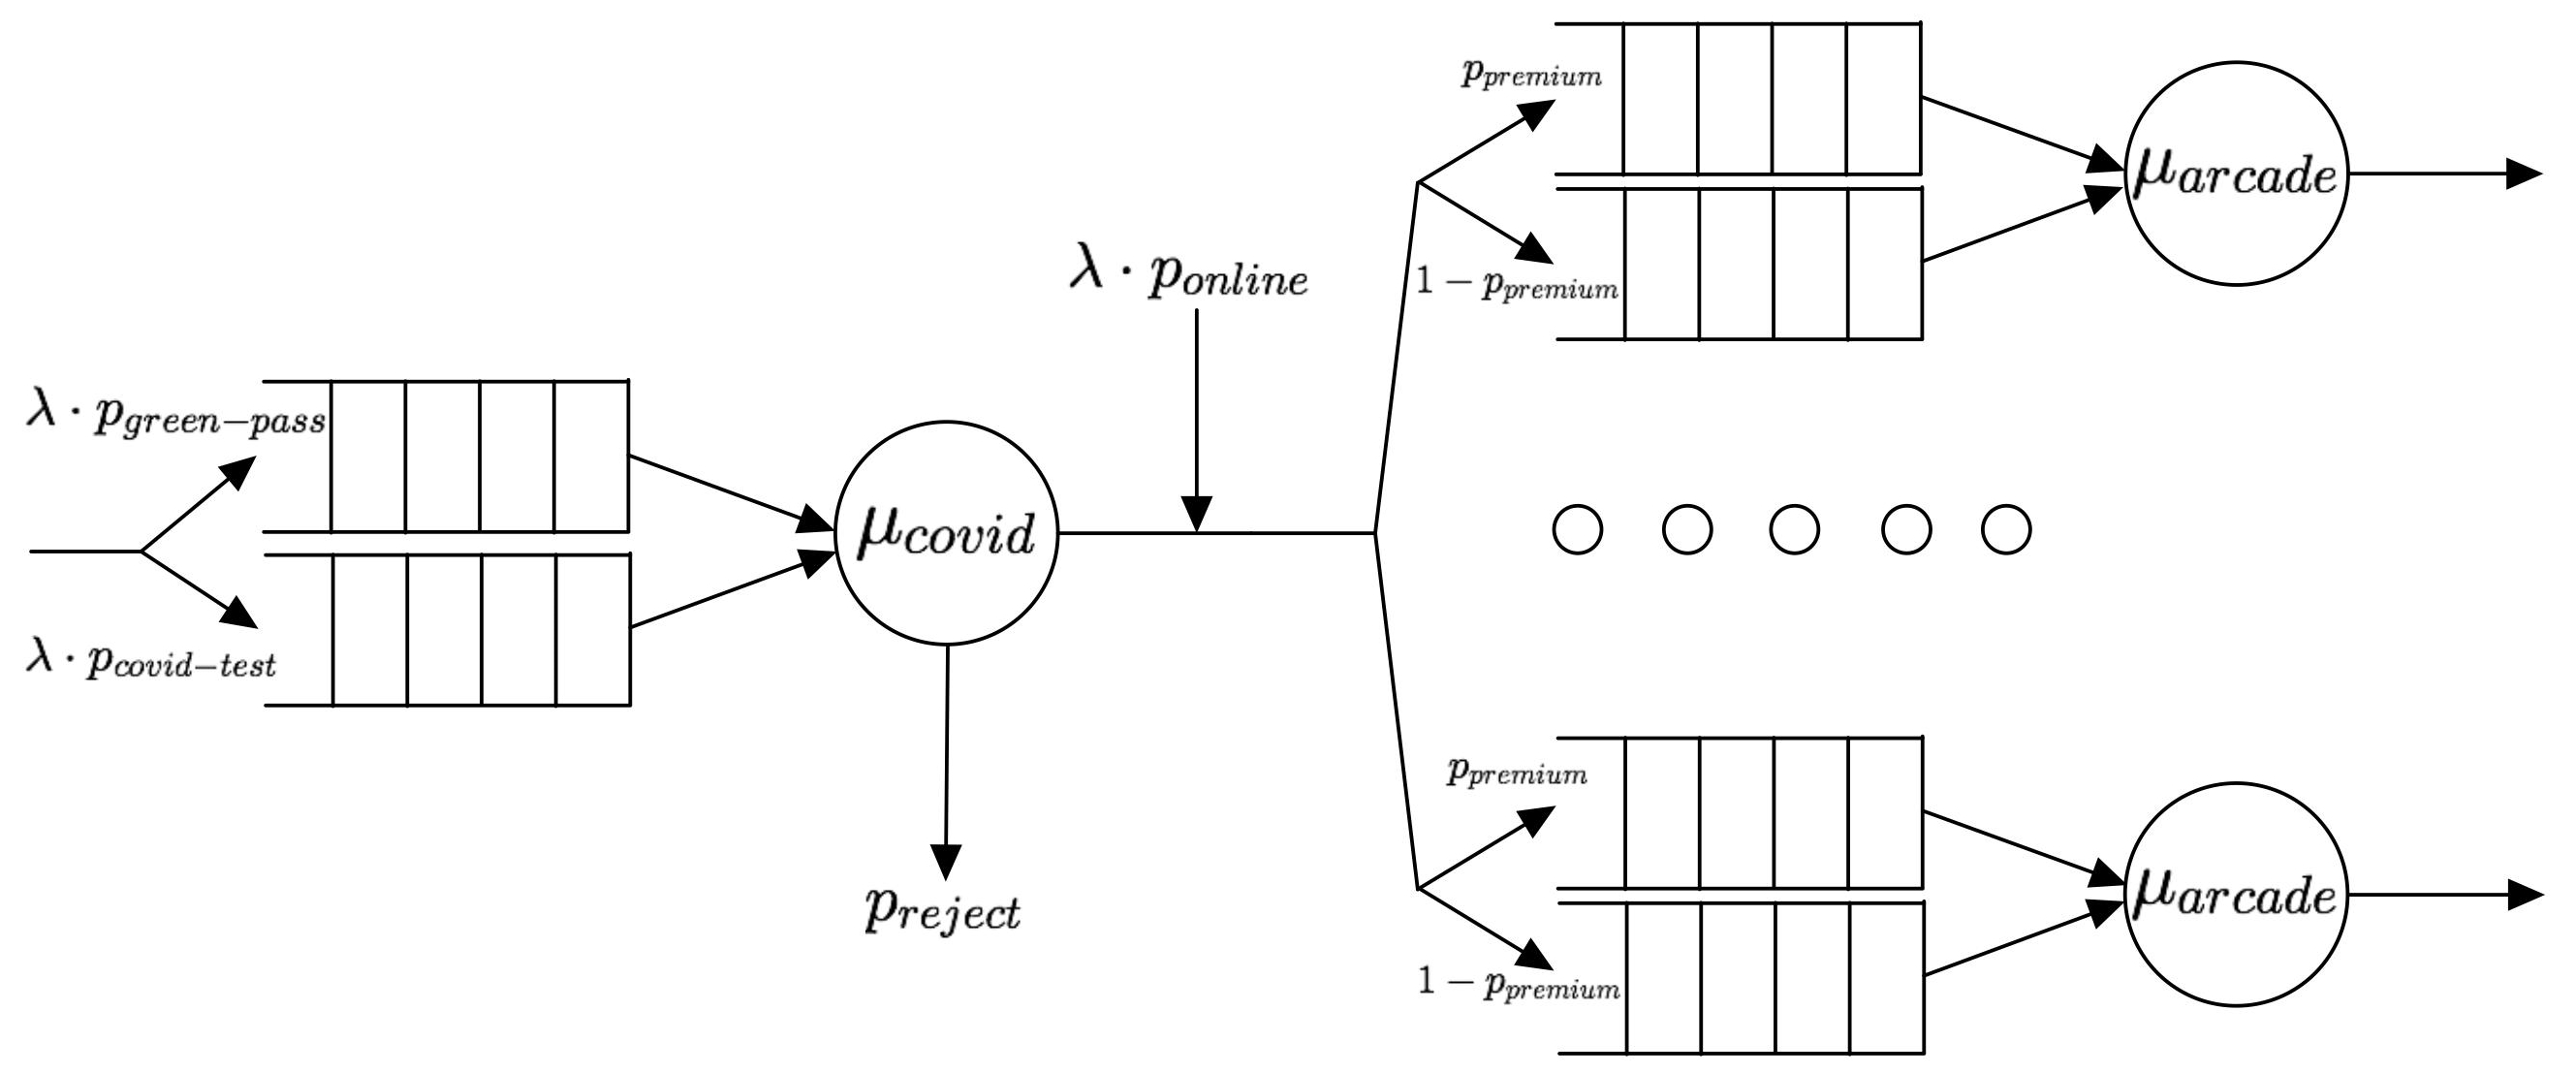
\includegraphics[scale=0.70]{images/adv_model_low_level.jpg}
	\caption{Advanced Model, Low-level view}\label{figura:adv_model_low_level}
\end{figure}

\subsection{Modello delle Specifiche}
Gli arrivi sono modellati con un processo di Poisson, con media variabile a seconda della fascia oraria. In particolare, la media per la prima fascia oraria è di $0.07143$  clienti/minuto (14 minuti/cliente), la media per la seconda fascia oraria è di $0.2$ clienti/minuto (5 minuti/cliente), la media per la terza fascia oraria è di $0.07143$ clienti/minuto (14 minuti/cliente), la media per la quarta fascia oraria è di $0.02857$  clienti/minuto (35 minuti/cliente).
\\ \\
La percentuale di clienti con biglietto online è del 20\%. La percentuale di clienti che si sottopone al controllo del  Green-pass è del 48\%. La percentuale di clienti che si sottopone al tampone è del 32\%.
\\ \\
La distribuzione del tempo di servizio per il controllo del green-pass è stata modellata
con una distribuzione Normale con media 2 minuti (0.5 clienti/minuto) e varianza 2.25 minuti, troncata tra 1 e 3 minuti. 
\\
La distribuzione del tempo di servizio per il tampone è stata modellata
con una distribuzione Normale con media 10 minuti (0.1 clienti/minuto) e varianza 2.25 minuti, troncata tra 8 e 12 minuti. 
\\
È stata scelta una Normale troncata con questi valori poiché permette di modellare un'operazione con bassa variabilità e di scartare valori eccessivamente piccoli o grandi che non rispecchierebbero tempi di servizio reali.
\\ \\
La distribuzione del tempo di servizio per un generico arcade è stata modellata
con una distribuzione Normale con media 15 minuti ($0.0\overline{6}$ clienti/minuto) e varianza 9 minuti, troncata tra 3 e 25 minuti.
\\ \\
La percentuale di clienti che acquista un biglietto premium è pari al 36\%.
\\ \\
La percentuale di clienti che risulta positiva al Covid-19 oppure presenta un green-pass non idoneo è in totale del 5\%.
\\ \\
Le probabilità per la scelta del node arcade è stata modellata tramite una distribuzione Uniforme in modo che ciascun servente abbia la stessa probabilità di essere selezionato. Questa scelta permette di mantenere circa la stessa utilizzazione per tutti i serventi dato che hanno lo stesso tasso di servizio.

\subsection{Modello Computazionale}
L’approccio di simulazione utilizzato è stato quello Next-Event Simulation. Il linguaggio di programmazione utilizzato è \textit{Python v.3.8}, facendo particolare riferimento alle librerie \ref{link} implementate dall’autore del libro di testo, e forniteci nel corso delle lezioni.
Il codice di base per la simulazione segue quanto descritto nell'algoritmo \ref{algo2}. Quest'ultimo si avvale di ulteriori strutture dati e funzioni necessarie al corretto funzionamento.

\begin{algorithm}[H]
\caption{Multiqueue Priority - Rete Aperta}\label{algo2}
\begin{algorithmic}[1]
\Procedure{Modello Avanzato}{}
\State $\textit{Inizializzazione clock}$
\State $\textit{Inizializzazione lista dei nodi}$
\State $\textit{Inizializzazione struttura Integrali}$
\State $\textit{Selezione nodo su cui generare il primo arrivo}$
\State $\textit{Selezione coda su cui generare il primo arrivo}$
\State $\textit{Generazione primo arrivo}$
\While{\textit{ultimo arrivo $<$ STOP} \textbf{or} \textit{ci sono job nel sistema}}
  \State $\textit{Scelta del prossimo evento}$
  \For{$i\gets 0, \textit{numero nodi}$}
    \If{$\textit{nodi non vuoti}$}
      \State $\textit{Aggiornamento statistiche}$
    \EndIf

  \EndFor
  \State $\textit{Avanzamento del clock}$
  \If{\textit{Evento} $= \textit{Cambio fascia oraria}$}
  \State $\textit{Selezione tasso arrivi corretto}$
  \EndIf
  \If{\textit{Evento} $= Arrivo$} \Comment{Arrivo}
    \State $\textit{Aggiornamento stato nodo e code di priorità}$ \Comment{Aggiornamento code di priorità}
    \State $\textit{Aggiornamento stato sistema}$
    \State $\textit{Selezione nodo prossimo arrivo}$
    \State $\textit{Selezione coda prossimo arrivo}$
    \If{\textit{Jobs nel centro} $= 1$}
    \State $\textit{Schedulazione prossimo servizio}$
    \EndIf
  \Else  \Comment{Completamento}
    \State $\textit{Aggiornamento stato nodo e code di priorità}$ \Comment{Aggiornamento code di priorità}
    \If{\textit{Nodo Arcade}}
      \State $\textit{Aggiornamento stato sistema}$
    \EndIf
    \If{\textit{Jobs nel centro} $> 0$}
      \State $\textit{Selezione nodo prossimo serivizo}$
      \State $\textit{Selezione coda prossimo servizio}$
    \EndIf
    \If{\textit{Nodo Covid-Check}}
      \If{\textit{Covid test negativo }\text{\textbf{and}} \textit{Green-pass valido}}
        \State $\textit{Aggiornamento stato sistema}$
      \EndIf
    \EndIf
  \EndIf
\EndWhile
\EndProcedure
\end{algorithmic}
\end{algorithm}

\subsection{Verifica}
Le strutture e le funzioni precedentemente accennate sono state sottoposte ad una fase di testing in modo da garantire il loro corretto funzionamento. Durante l'implementazione del progetto, l'applicazione iterativa di tale fase ha permesso di individuare e correggere diversi difetti, emersi a seguito del manifestarsi di malfunzionamenti del sistema.

\subsection{Validazione}
Al fine di validare il modello implementato, sono stati eseguiti diversi run variando determinati parametri. I risultati possono essere osservati in tabella \ref{tab4} e \ref{tab5}.

\begin{table}[htbp]
\caption{System statistics}
\begin{center}
\begin{tabular}{|c|c|c|c|}
\hline
\textbf{\# nodi arcades} & \textbf{avg interarrival time} & \textbf{avg wait} & \textbf{avg \# node} \\ \hline
\textbf{2} & 14.037119 & 27.424052 & 1.953673 \\ \hline
\textbf{5} & 14.037119 & 21.654822 & 1.542677 \\ \hline
\textbf{9} & 14.037119 &  20.727016 & 1.476581 \\ \hline
\multicolumn{4}{l}{$^{\mathrm{*}}$ $seed=1234567891, \lambda_{system} =\frac{1}{14} \frac{job}{min}, \# jobs=517028, $}
\end{tabular}
\label{tab4}
\end{center}
\end{table}

Per quanto riguarda la tabella \ref{tab4}, è possibile evincere come il tempo di interarrivo medio del sistema converga al parametro impostato $\lambda_{system}^{-1}$.

\begin{table}[H]
\caption{Arcades statistics}
\begin{center}
\begin{tabular}{|c|c|c|c|c|c|c|c|c|}
\hline
\textbf{\# nodi} & \multicolumn{2}{|c|}{\textbf{avg interarrival}} & \multicolumn{2}{|c|}{\textbf{avg wait}} & \multicolumn{2}{|c|}{\textbf{avg \# node}} & \multicolumn{2}{|c|}{\textbf{avg \# queue}} \\ \cline{2-9} 
\textbf{arcades} & \textbf{Priority} & \textbf{N Priority} & \textbf{Priority} & \textbf{N Priority} & \textbf{Priority} & \textbf{N Priority}& \textbf{Priority} & \textbf{N Priority}\\ \hline
2 & 81.467323 & 45.547404 & 17.803708 & 22.031882 & 0.218535 & 0.483710 & 0.034664 & 0.154467\\ \hline
5 & 205.391722 & 113.252959 & 15.827623 & 16.397222 & 0.077060 & 0.144781 & 0.004122 & 0.012311\\ \hline
9 & 370.111505 & 203.980331 & 15.425839 & 15.681829 & 0.041678 & 0.076871 & 0.001129 & 0.003296\\ \hline
\multicolumn{9}{l}{$^{\mathrm{*}}$ $seed=1234567891, \lambda_{system} =\frac{1}{14} \frac{job}{min}, \# jobs=517028 $.}
\end{tabular}
\label{tab5}
\end{center}
\end{table}


Per quanto riguarda la tabella \ref{tab5}, si può notare come la relazione di Little, applicabile in quanto il modello soddisfa le condizioni sufficienti, sia soddisfatta e come l'utilizzazione e il tempo di interarrivo medio, rispettivamente, decresca ed aumenti al crescere del numero degli arcade. Tale comportamento è giustificato dal fatto che i jobs vengono distribuiti in modo equiprobabile tra i diversi nodi arcade.
\\ \\
Come è possibile osservare dalle tabelle, inoltre, all'aumentare dei nodi nel sistema i tempi di attesa e il numero di jobs nei rispettivi centri diminuisce coerentemente a ciò che ci si aspetta.
\\ \\
Inoltre si può constatare che tutte le statistiche risultano inferiori nel caso prioritario, in conformità con quanto ci si figuri.

\subsection{Esperimenti di Simulazione}
%----Introduzione
Al fine di raggiungere gli obiettivi prefissati, è utile effettuare degli esperimenti di simulazione, utilizzando la configurazione ottimale dello studio precedente.

\subsubsection{Analisi del comportamento transiente}
%----Minimo n per stazionarietà
Attraverso l'analisi del comportamento transiente viene studiato il tempo medio di risposta del sistema, per ogni fascia oraria, utilizzando il metodo delle repliche.
In particolare, vengono effettuate run di simulazione
consecutive, utilizzando ogni volta come punto di partenza lo stato del sistema raggiunto dalla replica precedente. Il seed, infatti, viene settato una volta, all'inizio della prima replica.
La tecnica delle repliche permette di calcolare stime puntuali e intervallari ad ogni acquisizione, ognuna di queste corrispondente ad un certo numero di richieste processate.
\\ \\
Per quanto riguarda la prima fascia e la terza fascia oraria, rispettivamente (08:00-12:00) e (17:00-22:00), è possibile osservare i risultati dell'analisi in figura \ref{figura:adv_avg_ws_mor_s}. Tali fasce, infatti, hanno lo stesso $\lambda_{arrival}$ da modellazione.

\begin{figure}[H]
\centering
\captionsetup{justification=centering,margin=2cm}
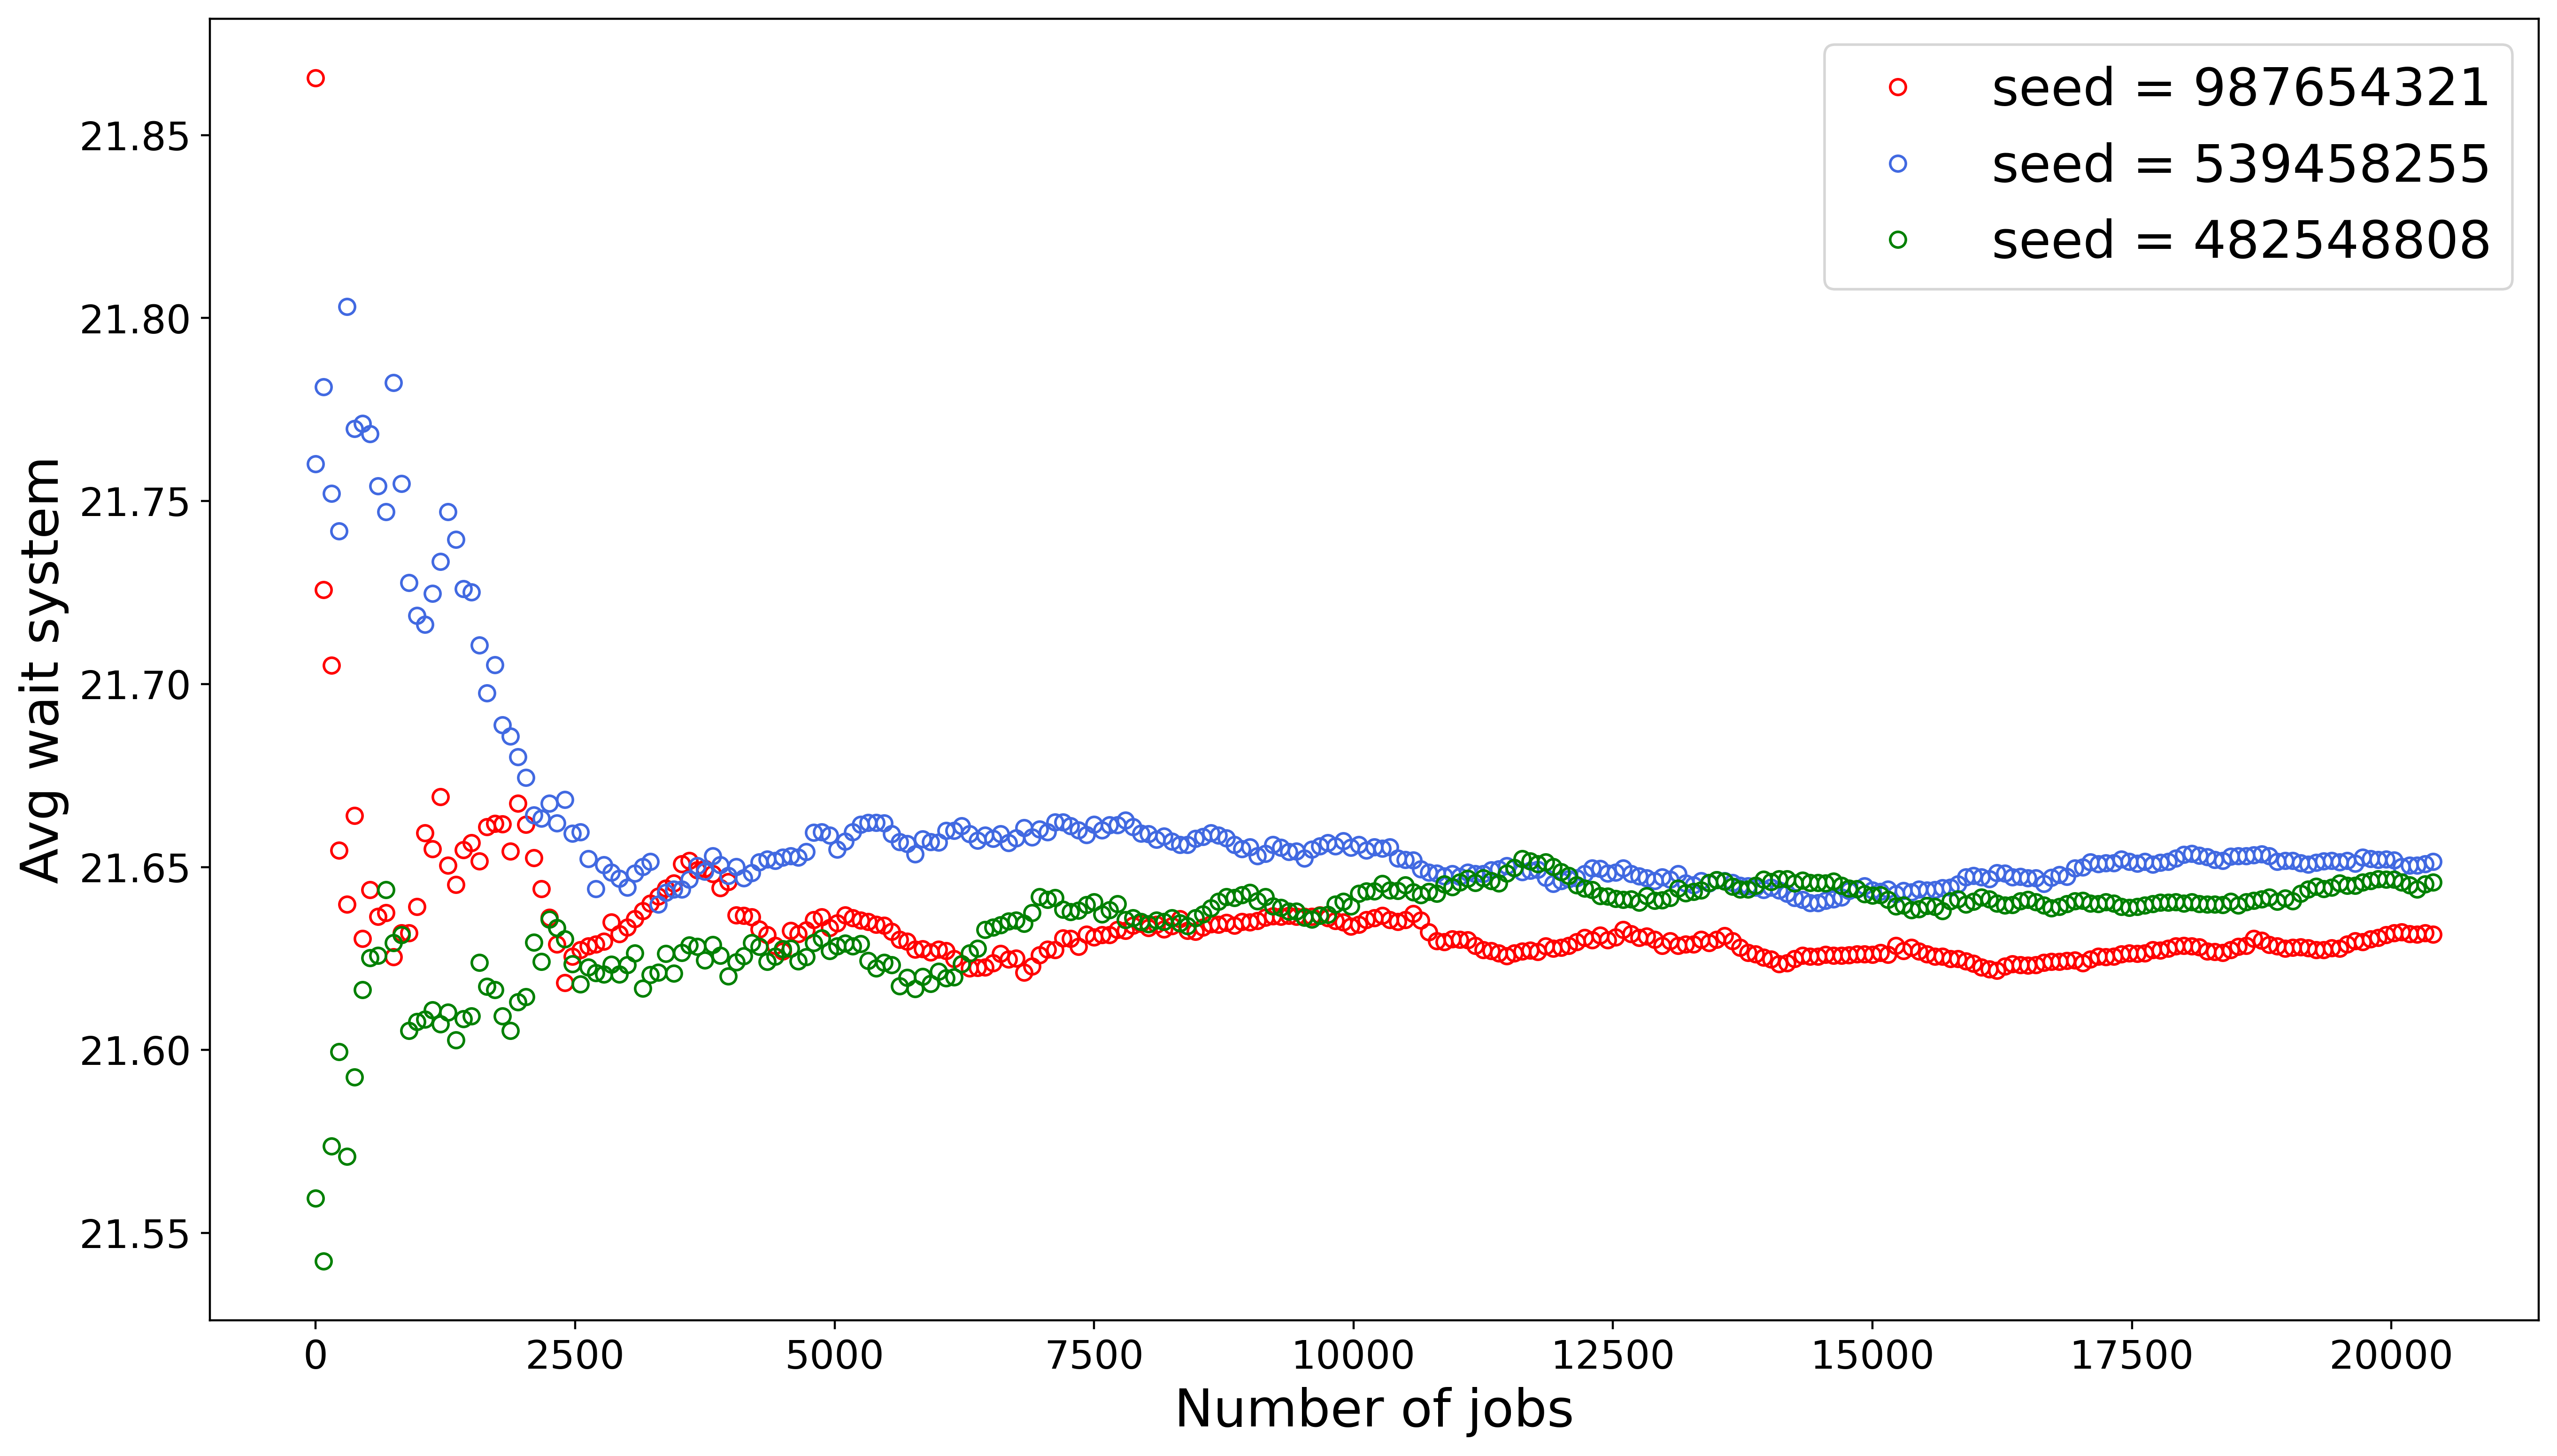
\includegraphics[scale=0.48]{images/adv_avg_ws_mor_s.png}
\caption{Average Wait System, 08:00-12:00 \& 17:00-22:00, $\lambda_{arrival}=\frac{1}{14} \frac{job}{min}$, Arcades: 5, repliche=64, Sampling\_freq=75}\label{figura:adv_avg_ws_mor_s}
\end{figure}


Per quanto riguarda la seconda fascia oraria (12:00-17:00), è possibile osservare i risultati dell'analisi in figura \ref{figura:adv_avg_ws_aft_s}.



\begin{figure}[H]
\centering
\captionsetup{justification=centering,margin=2cm}
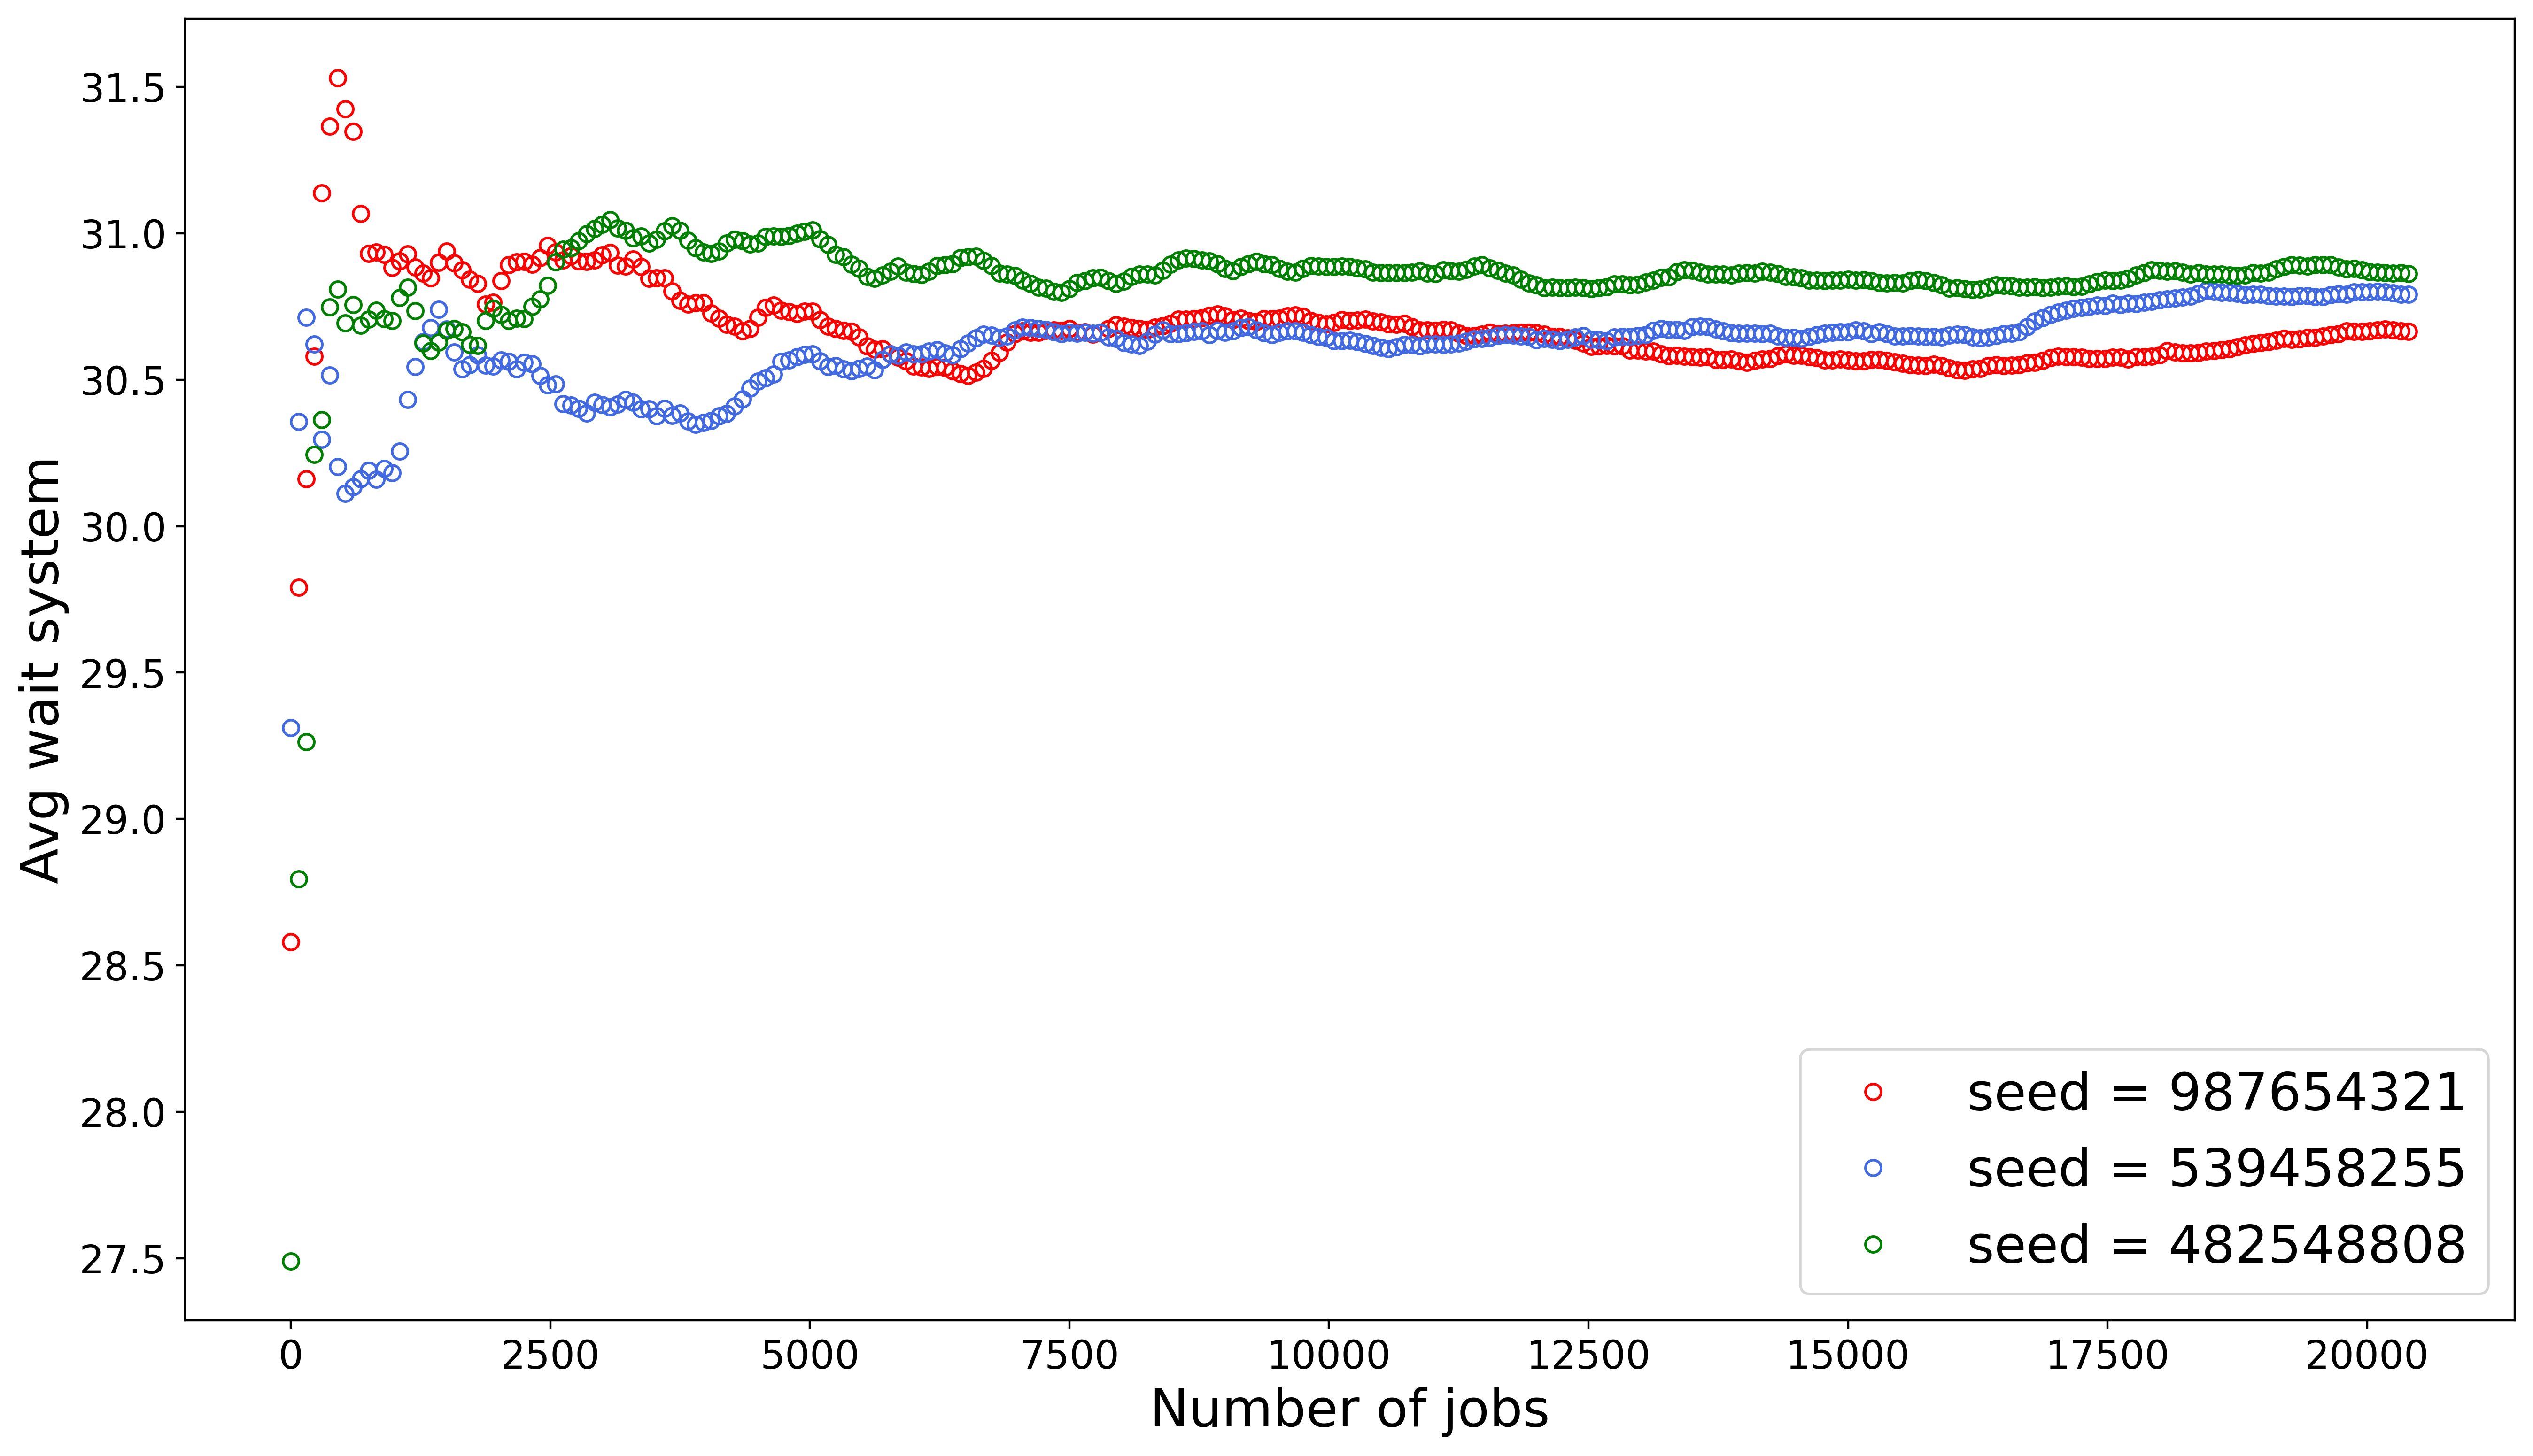
\includegraphics[scale=0.48]{images/adv_avg_ws_aft_s.png}
\caption{Average Wait System, 12:00-17:00, $\lambda_{arrival}=\frac{1}{5} \frac{job}{min}$, Arcades: 12, repliche=64, Sampling\_freq=75}\label{figura:adv_avg_ws_aft_s}
\end{figure}


Per quanto riguarda la quarta fascia oraria (22:00-08:00), è possibile osservare i risultati dell'analisi in figura \ref{figura:adv_avg_ws_night_s}.


\begin{figure}[H]
\centering
\captionsetup{justification=centering,margin=2cm}
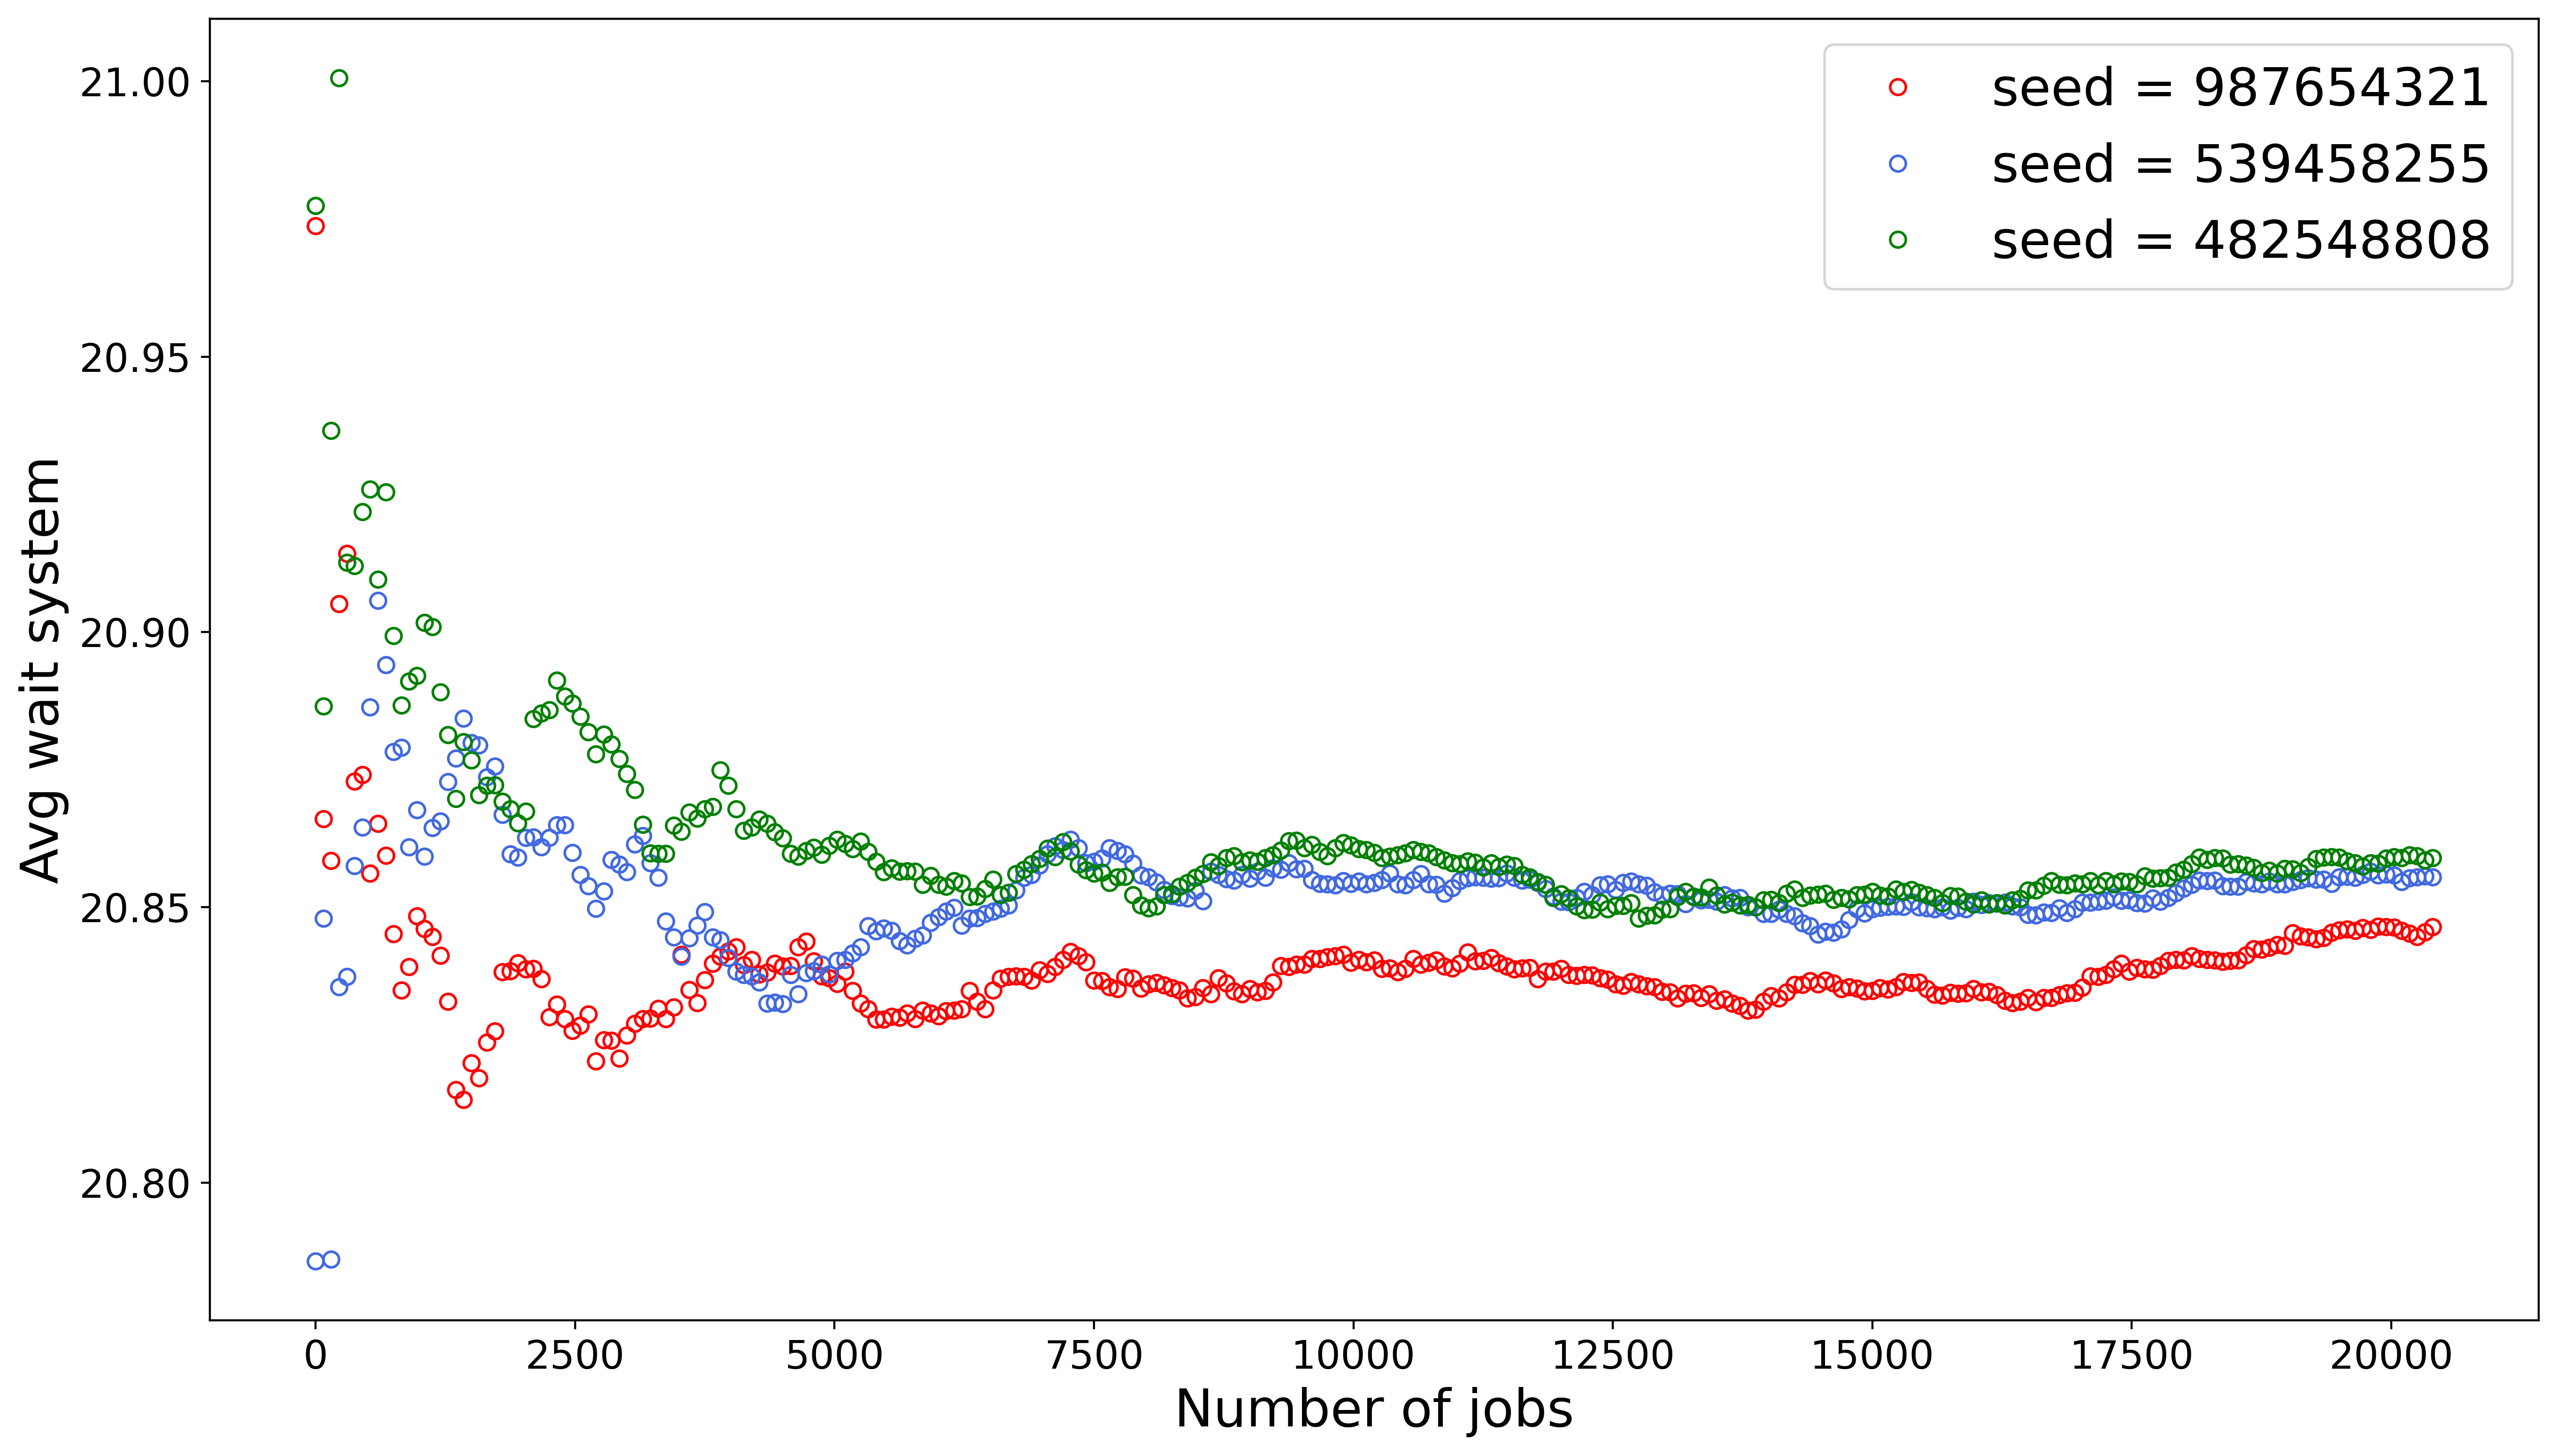
\includegraphics[scale=0.48]{images/adv_avg_ws_night_s.png}
\caption{Average Wait System, 22:00-08:00, $\lambda_{arrival}=\frac{1}{35} \frac{job}{min}$, Arcades: 2, repliche=64, Sampling\_freq=75}\label{figura:adv_avg_ws_night_s}
\end{figure}

Come si evince dai risultati dell'analisi, il modello avanzato, come previsto, raggiunge la stazionarietà utilizzando la configurazione ottimale ottenuta nel modello base.



\subsubsection{Analisi del comportamento stazionario}
Considerati i risultati dell'analisi transiente, è possibile procedere allo studio del comportamento stazionario.
Attraverso l'analisi del comportamento stazionario si vuole confrontare, con la configurazione ottima di nodi arcade, per ogni fascia oraria, i tempi di attesa nella coda Covid-19 sperimentati dagli utenti con green-pass, per quanto riguarda il modello base e quello avanzato, verificando che l'obiettivo 2 in \ref{Advanced_Goal} venga raggiunto.

In questa fase sono state effettuate simulazioni con tempi
d’osservazione molto lunghi, utilizzando la tecnica batch-means per ottenere delle stime degli indici di prestazione in regime stazionario, evitando la problematica del bias dovuto alle condizioni iniziali del sistema. Cruciale in questa fase la scelta di due parametri: \textit{b} e \textit{k}, rispettivamente la grandezza del batch e il numero di batch in cui si divide la simulazione. Per la scelta di \textit{b} è stata utilizzata la linea guida di Banks, Carson, Nelson, e Nicol (2001), la quale afferma che il batch size venga aumentato fintantoché l'autocorrelazione a lag 1 tra batch means sia minore di 0.2. Nel caso in esame è stato constatato che tale direttiva viene rispettata con un \textit{b} pari a 256.
Per la scelta del parametro \textit{k} è stato usato il valore pari a 64 come consigliato dalle linee guida.
\\ \\
In seguito per ogni fascia oraria viene riportato il grafico relativo al tempo medio di attesa nella coda Covid-19 per i clienti dotati di green-pass, per ogni seed, per il modello base e il modello avanzato,con un intervallo di confidenza pari al $95\%$.

\begin{figure}[H]
	\centering
	\captionsetup{justification=centering,margin=2cm}
	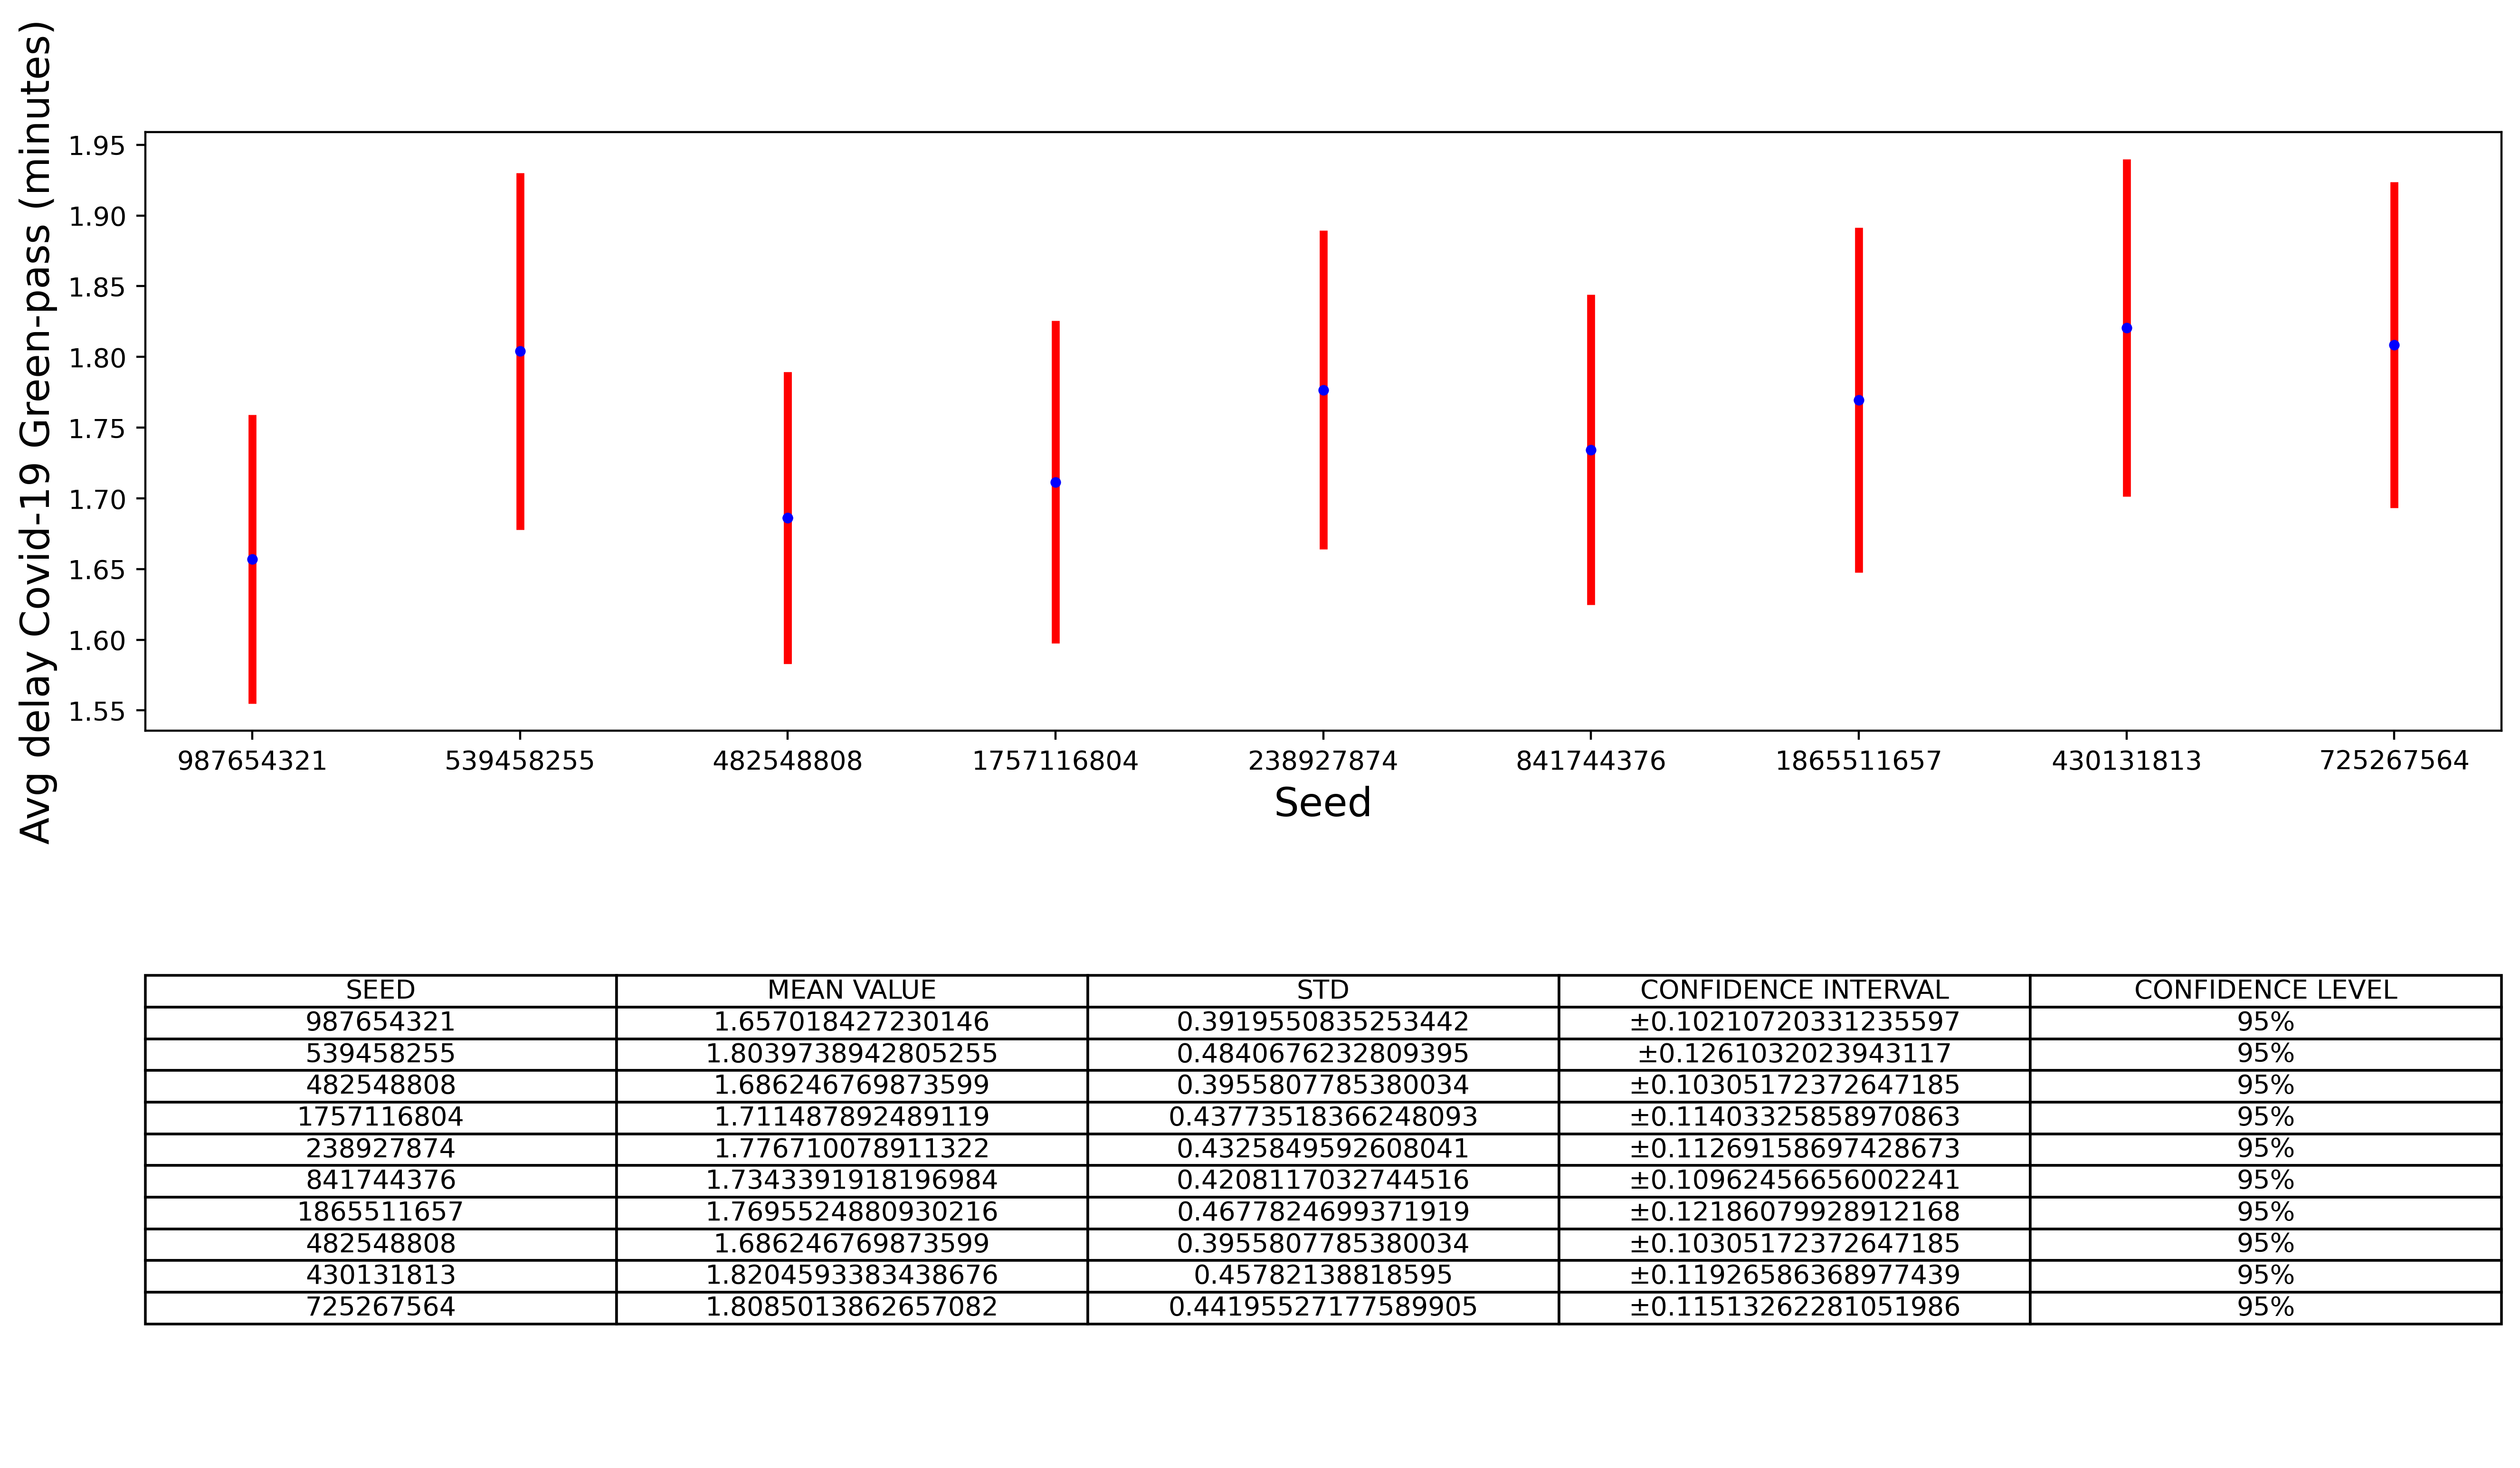
\includegraphics[scale=0.48]{images/avg_d_covid_steady_state_mor.png}
	\caption{Base Model, Average delay Covid-19 Green-Pass, 08:00-12:00 \& 17:00-22:00, $\lambda_{arrival}=\frac{1}{14} \frac{job}{min}$, b=256, k=64}\label{figura:avg_d_covid_steady_state_mor}
\end{figure}

\begin{figure}[H]
	\centering
	\captionsetup{justification=centering,margin=2cm}
	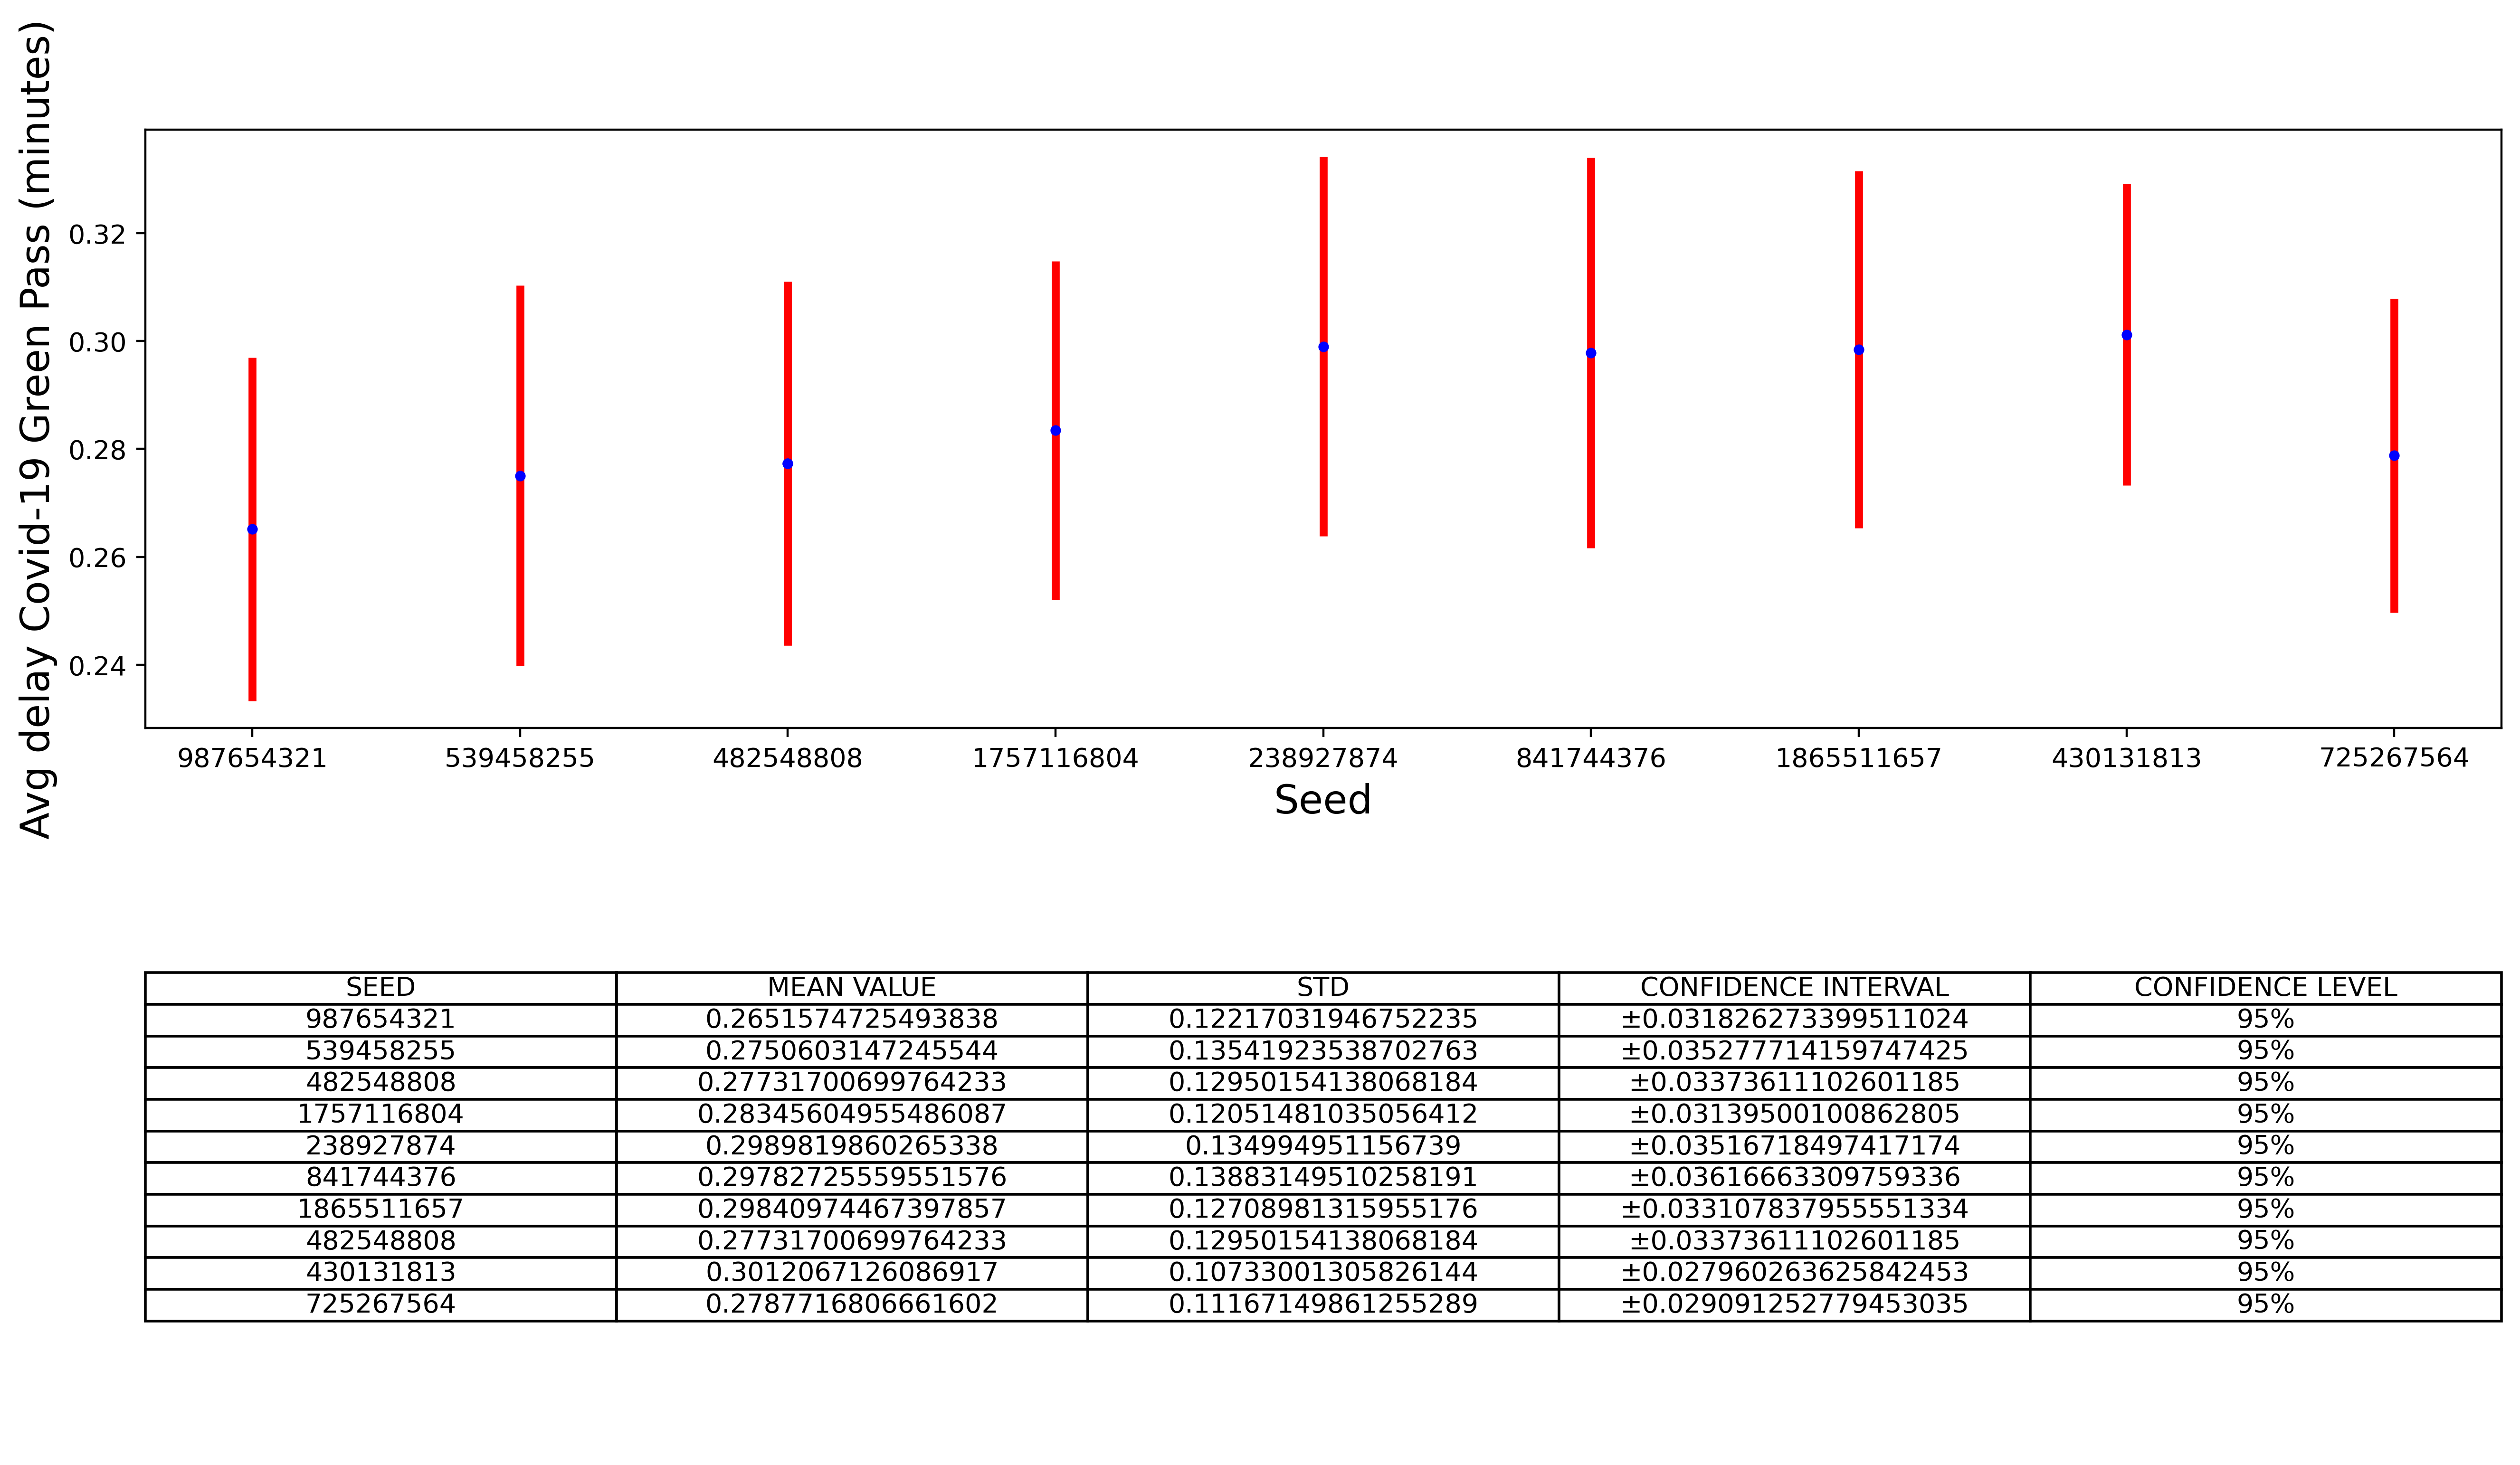
\includegraphics[scale=0.48]{images/adv_avg_d_covid_steady_state_mor.png}
	\caption{Advanced Model, Average delay Covid-19 Green-Pass, 08:00-12:00 \& 17:00-22:00, $\lambda_{arrival}=\frac{1}{14} \frac{job}{min}$, b=256, k=64}\label{figura:adv_avg_d_covid_steady_state_mor}
\end{figure}

\begin{figure}[H]
	\centering
	\captionsetup{justification=centering,margin=2cm}
	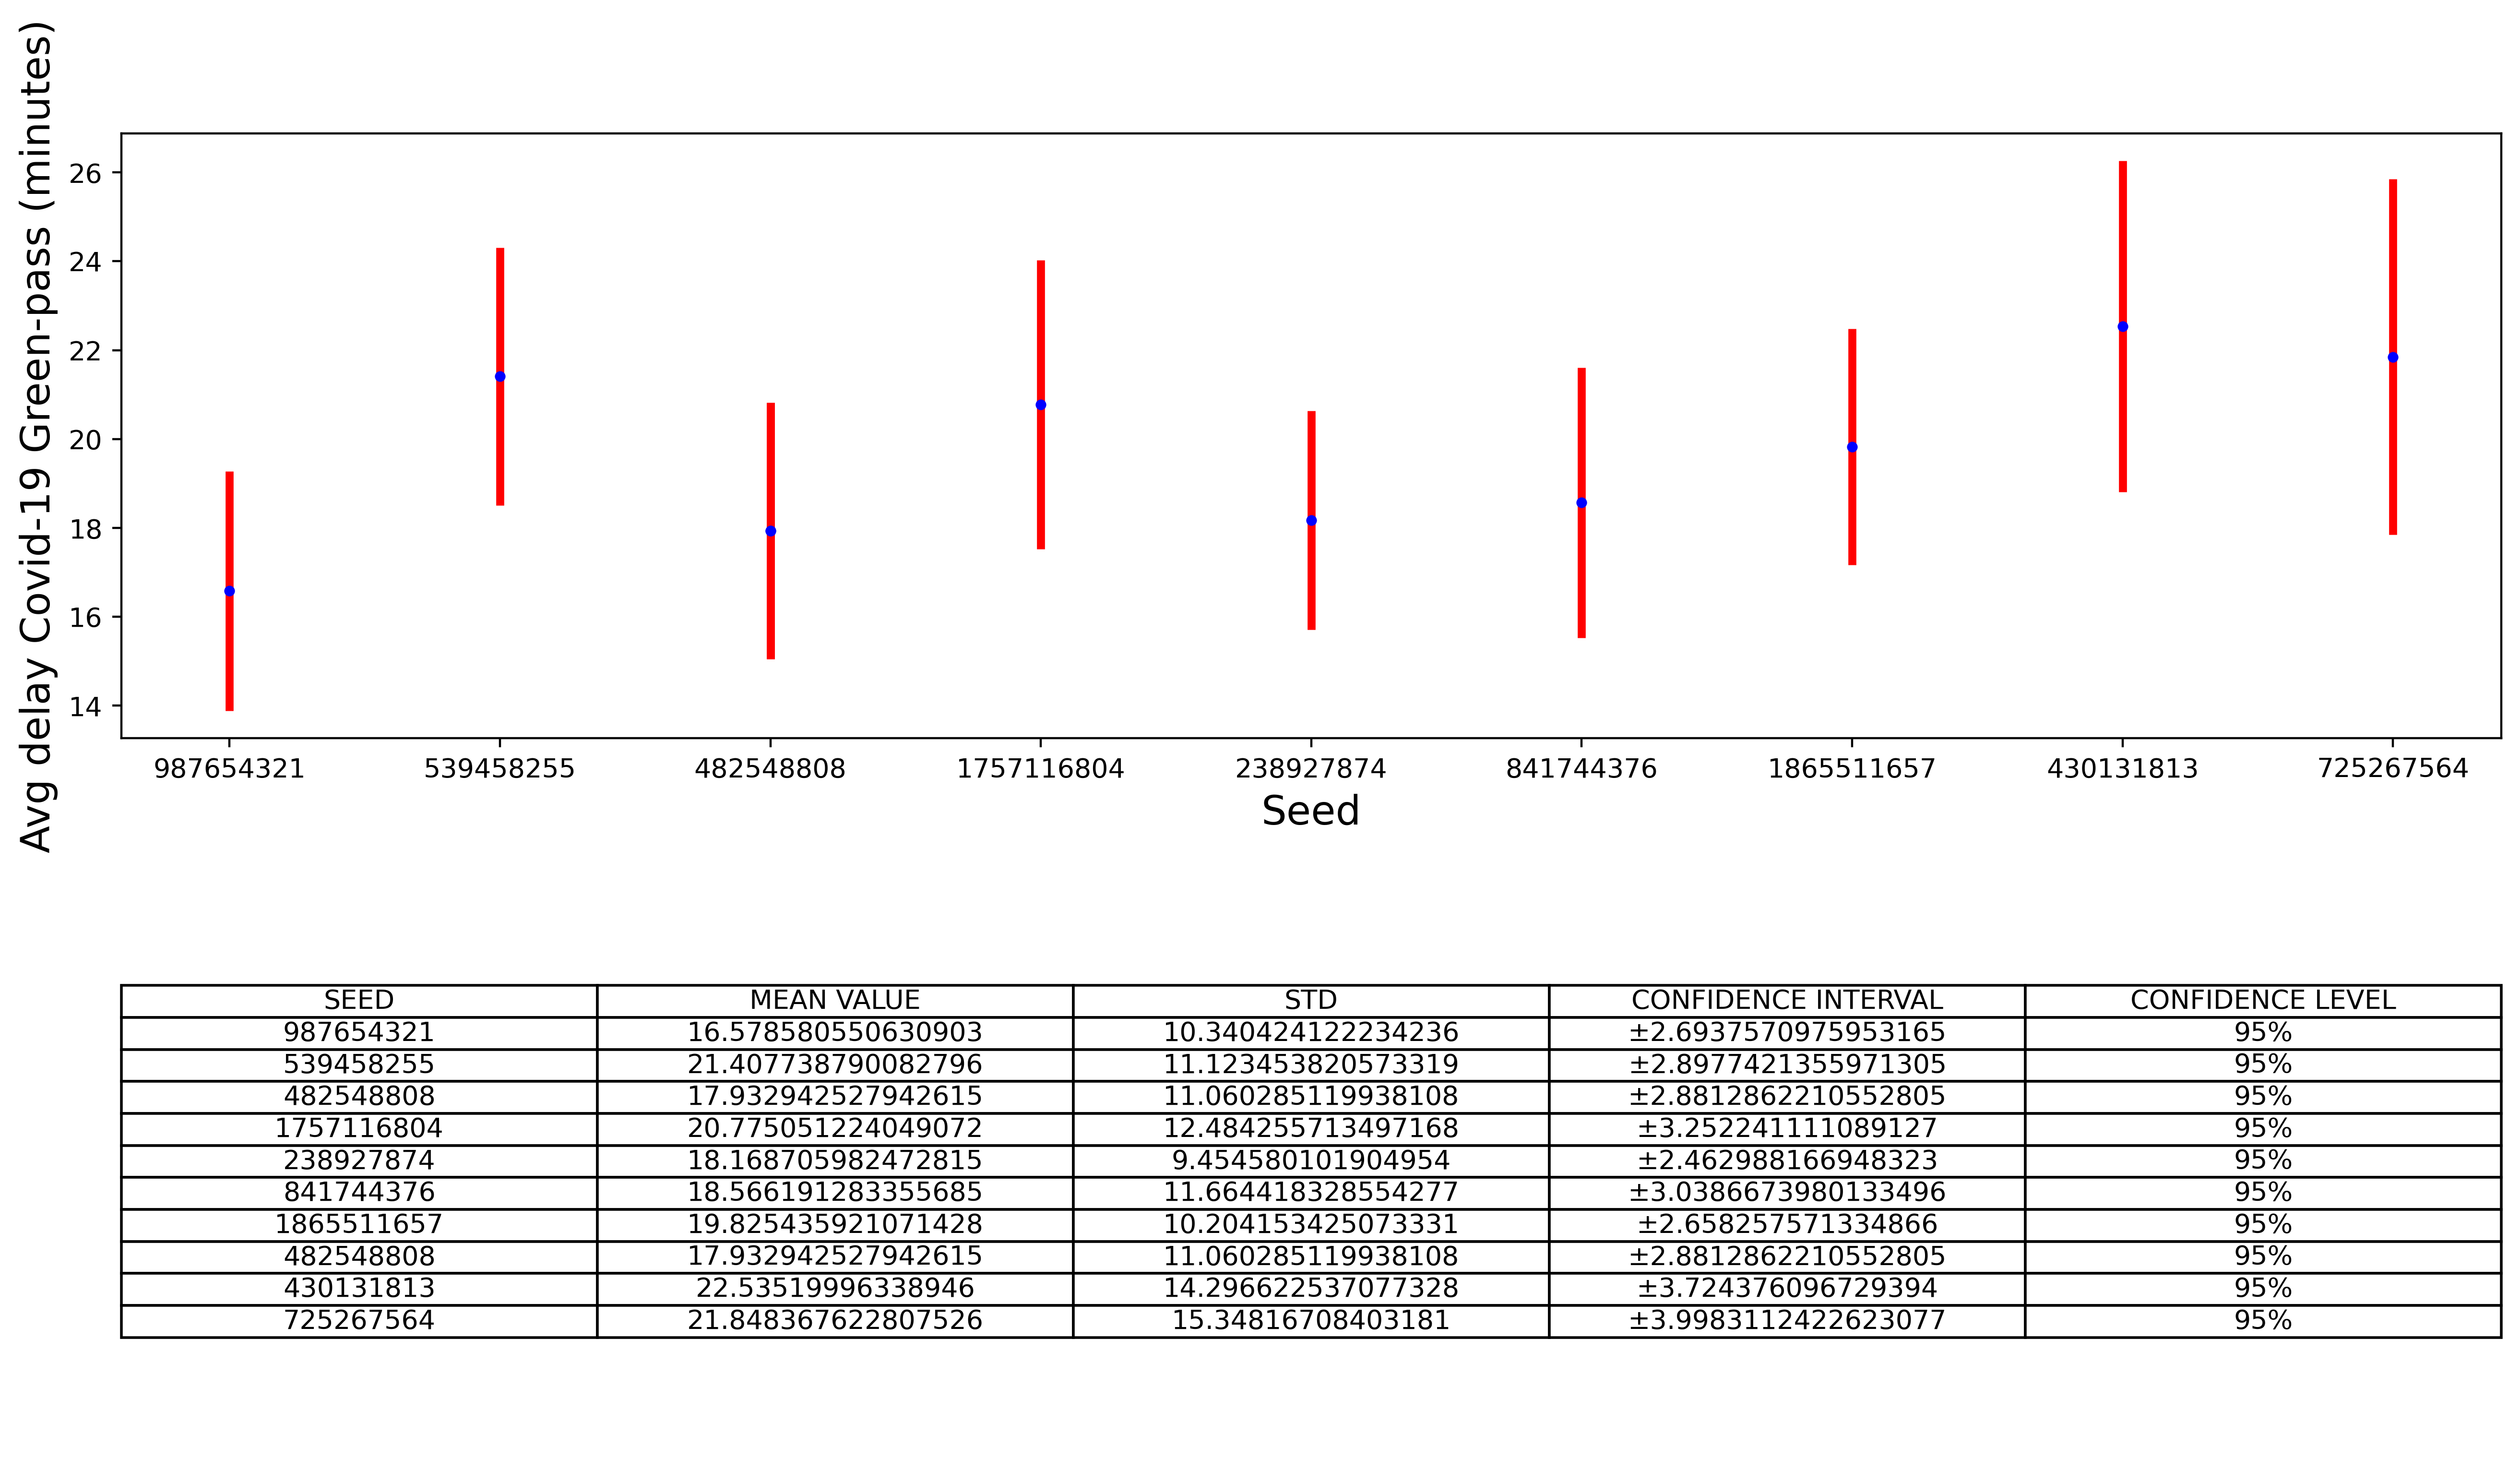
\includegraphics[scale=0.48]{images/avg_d_covid_steady_state_aft.png}
	\caption{Base Model, Average delay Covid-19 Green-Pass, 12:00-17:00, $\lambda_{arrival}=\frac{1}{5} \frac{job}{min}$, b=256, k=64}\label{figura:avg_d_covid_steady_state_aft}
\end{figure}

\begin{figure}[H]
	\centering
	\captionsetup{justification=centering,margin=2cm}
	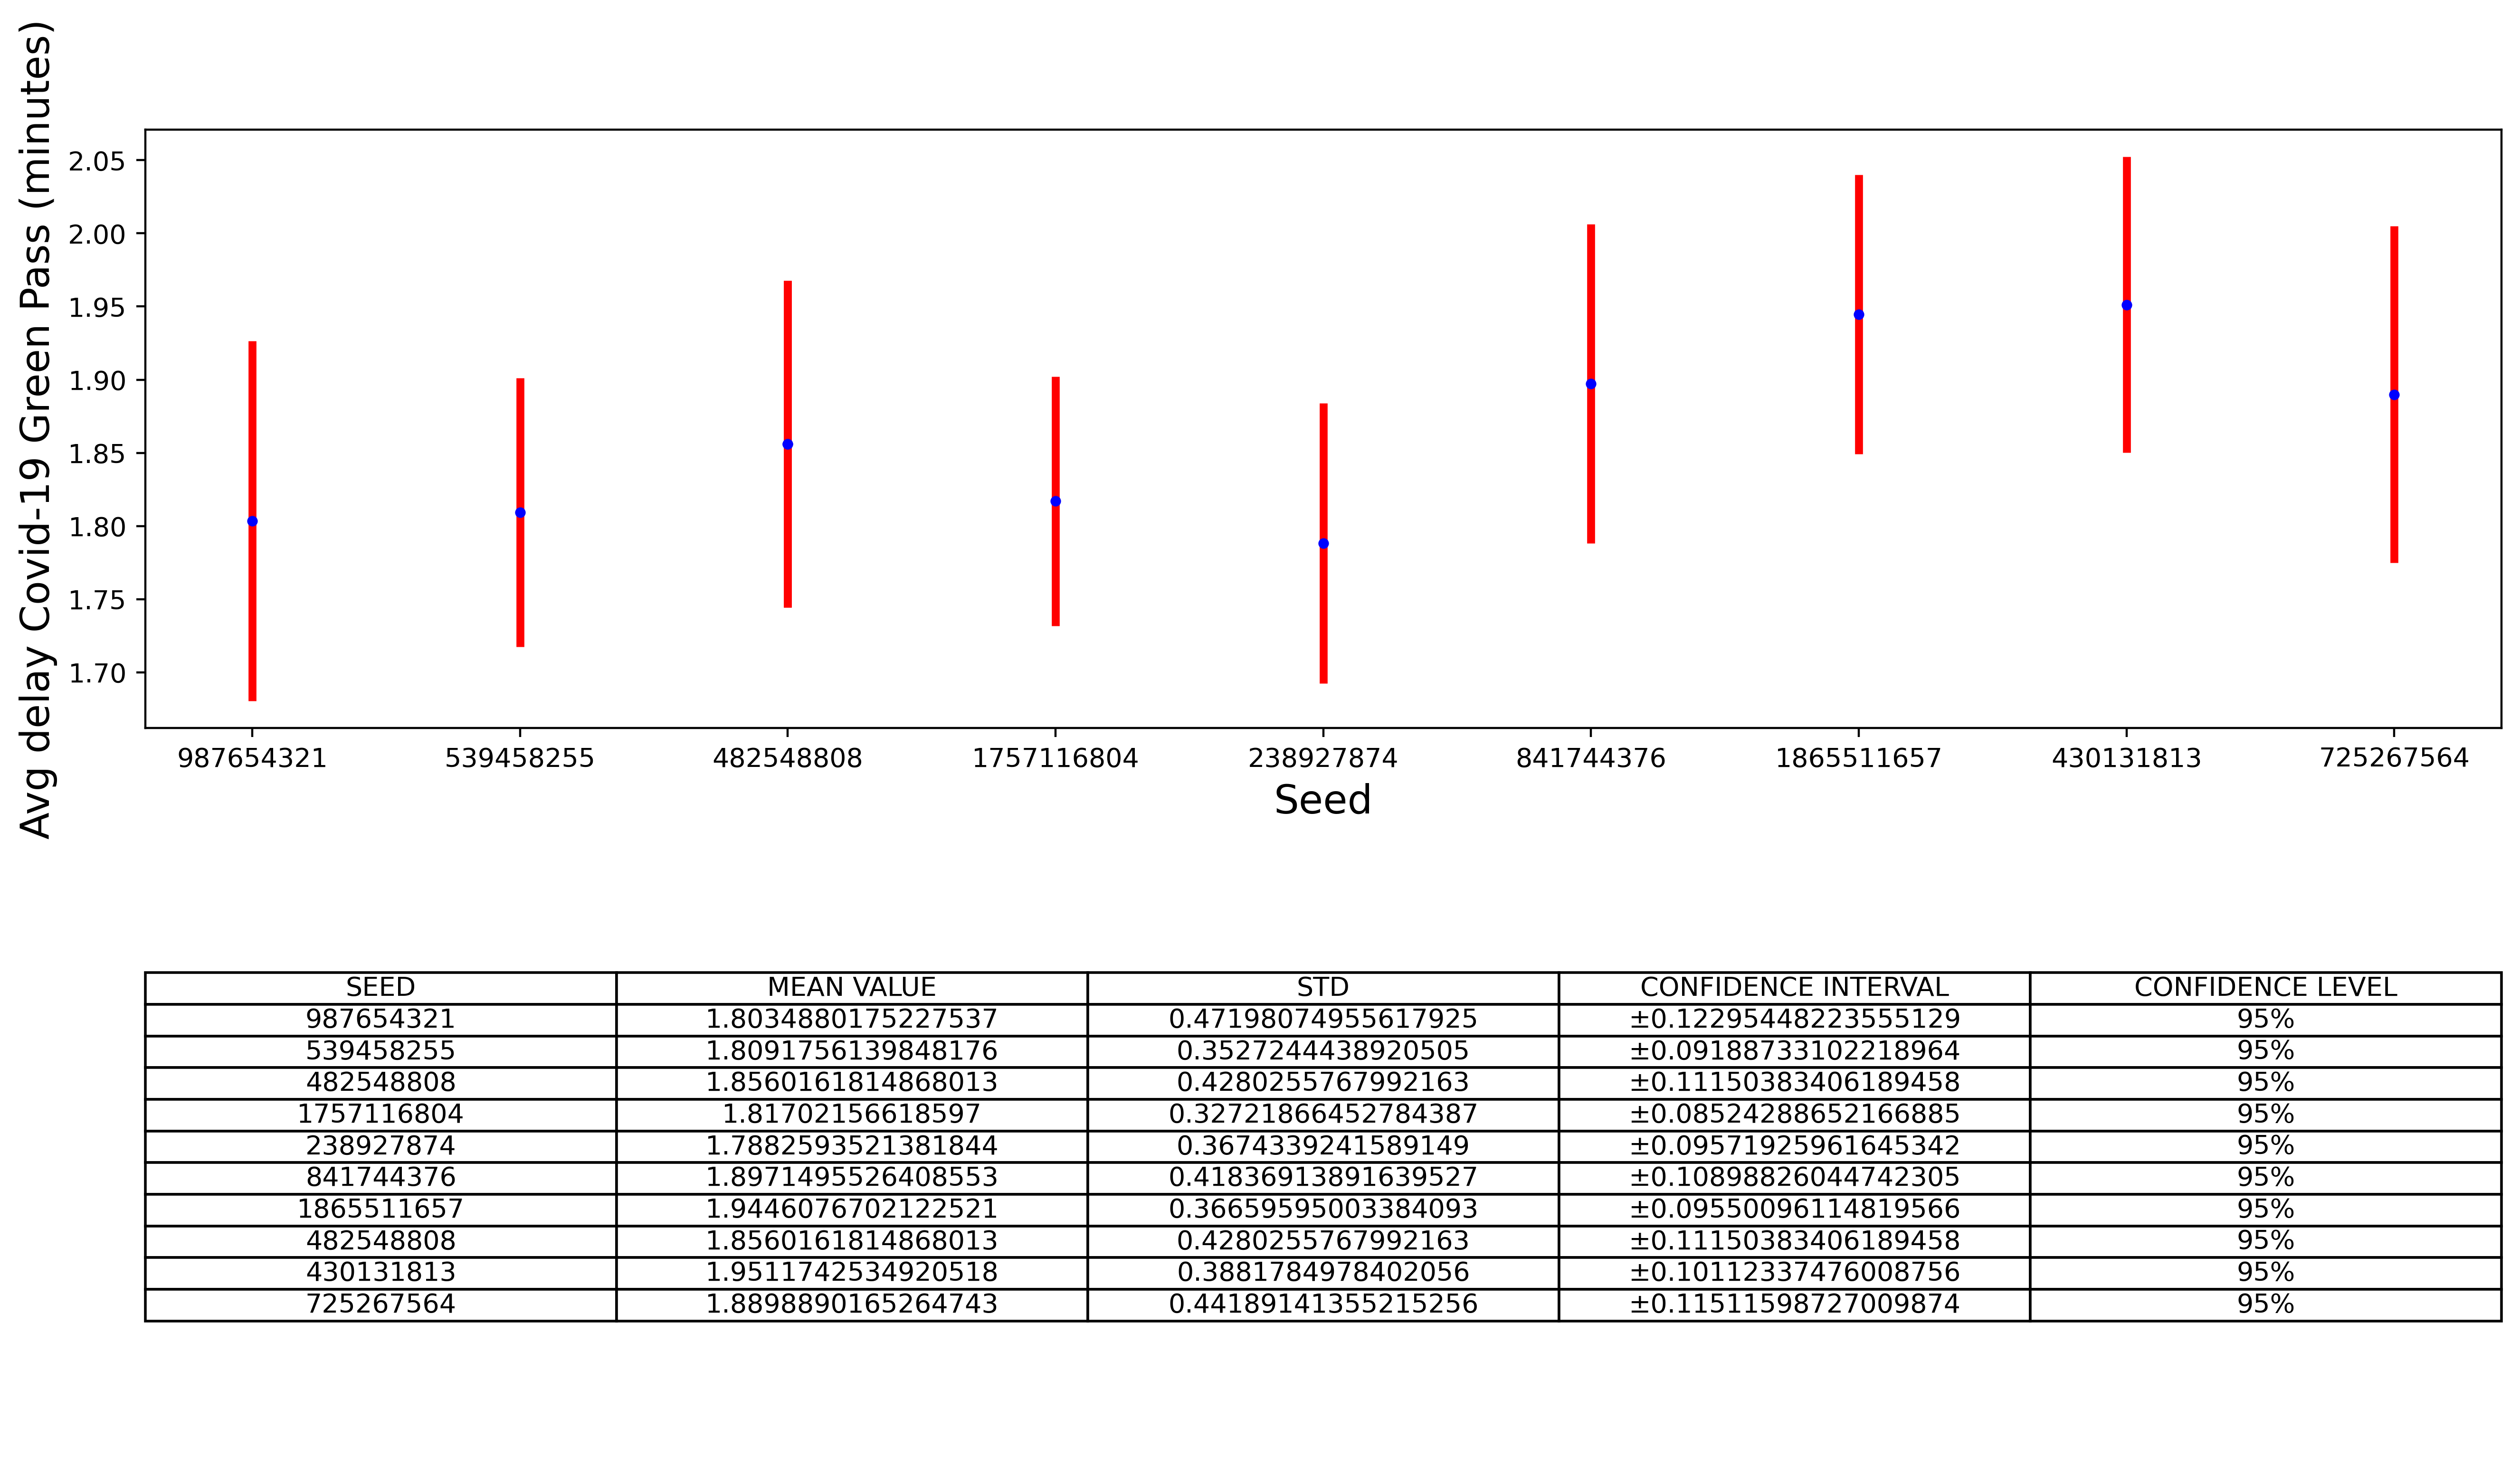
\includegraphics[scale=0.48]{images/adv_avg_d_covid_steady_state_aft.png}
	\caption{Advanced Model, Average delay Covid-19 Green-Pass, 12:00-17:00, $\lambda_{arrival}=\frac{1}{5} \frac{job}{min}$, b=256, k=64}\label{figura:adv_avg_d_covid_steady_state_aft}
\end{figure}

\begin{figure}[H]
	\centering
	\captionsetup{justification=centering,margin=2cm}
	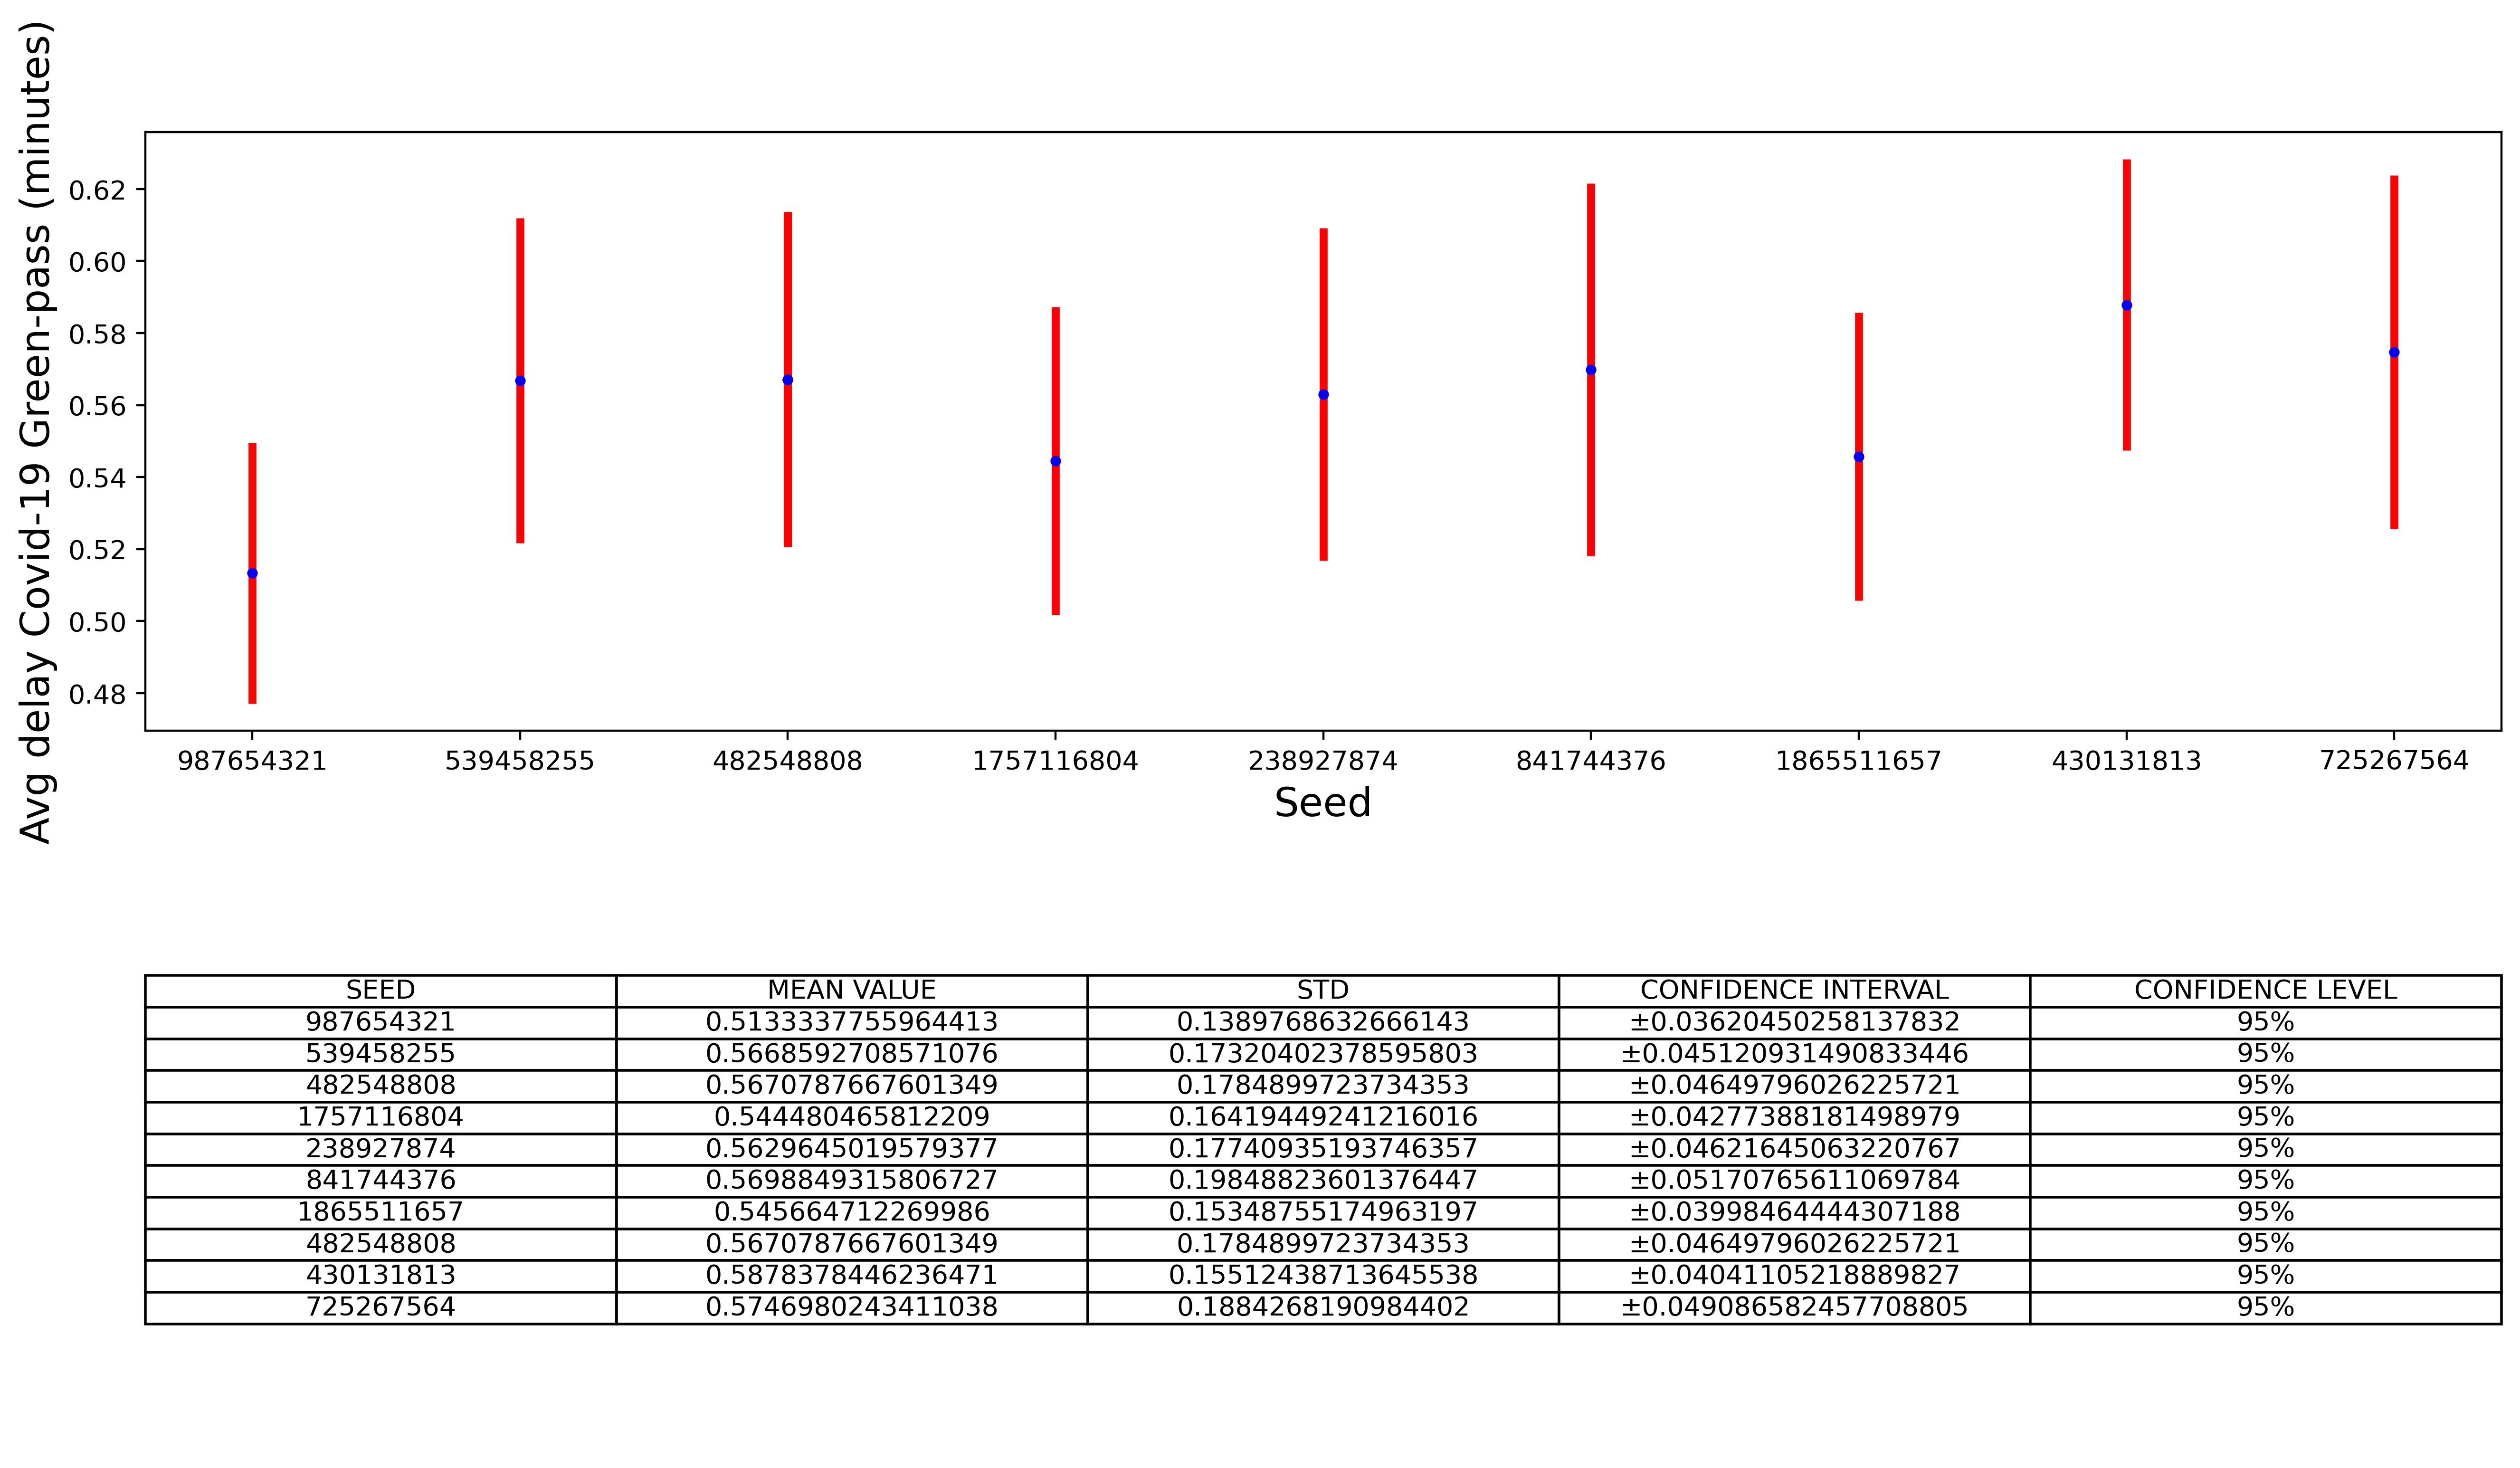
\includegraphics[scale=0.48]{images/avg_d_covid_steady_state_night.png}
	\caption{Base Model, Average delay Covid-19 Green-Pass, 22:00-08:00, $\lambda_{arrival}=\frac{1}{35} \frac{job}{min}$, b=256, k=64}\label{figura:avg_d_covid_steady_state_night}
\end{figure}

\begin{figure}[H]
	\centering
	\captionsetup{justification=centering,margin=2cm}
	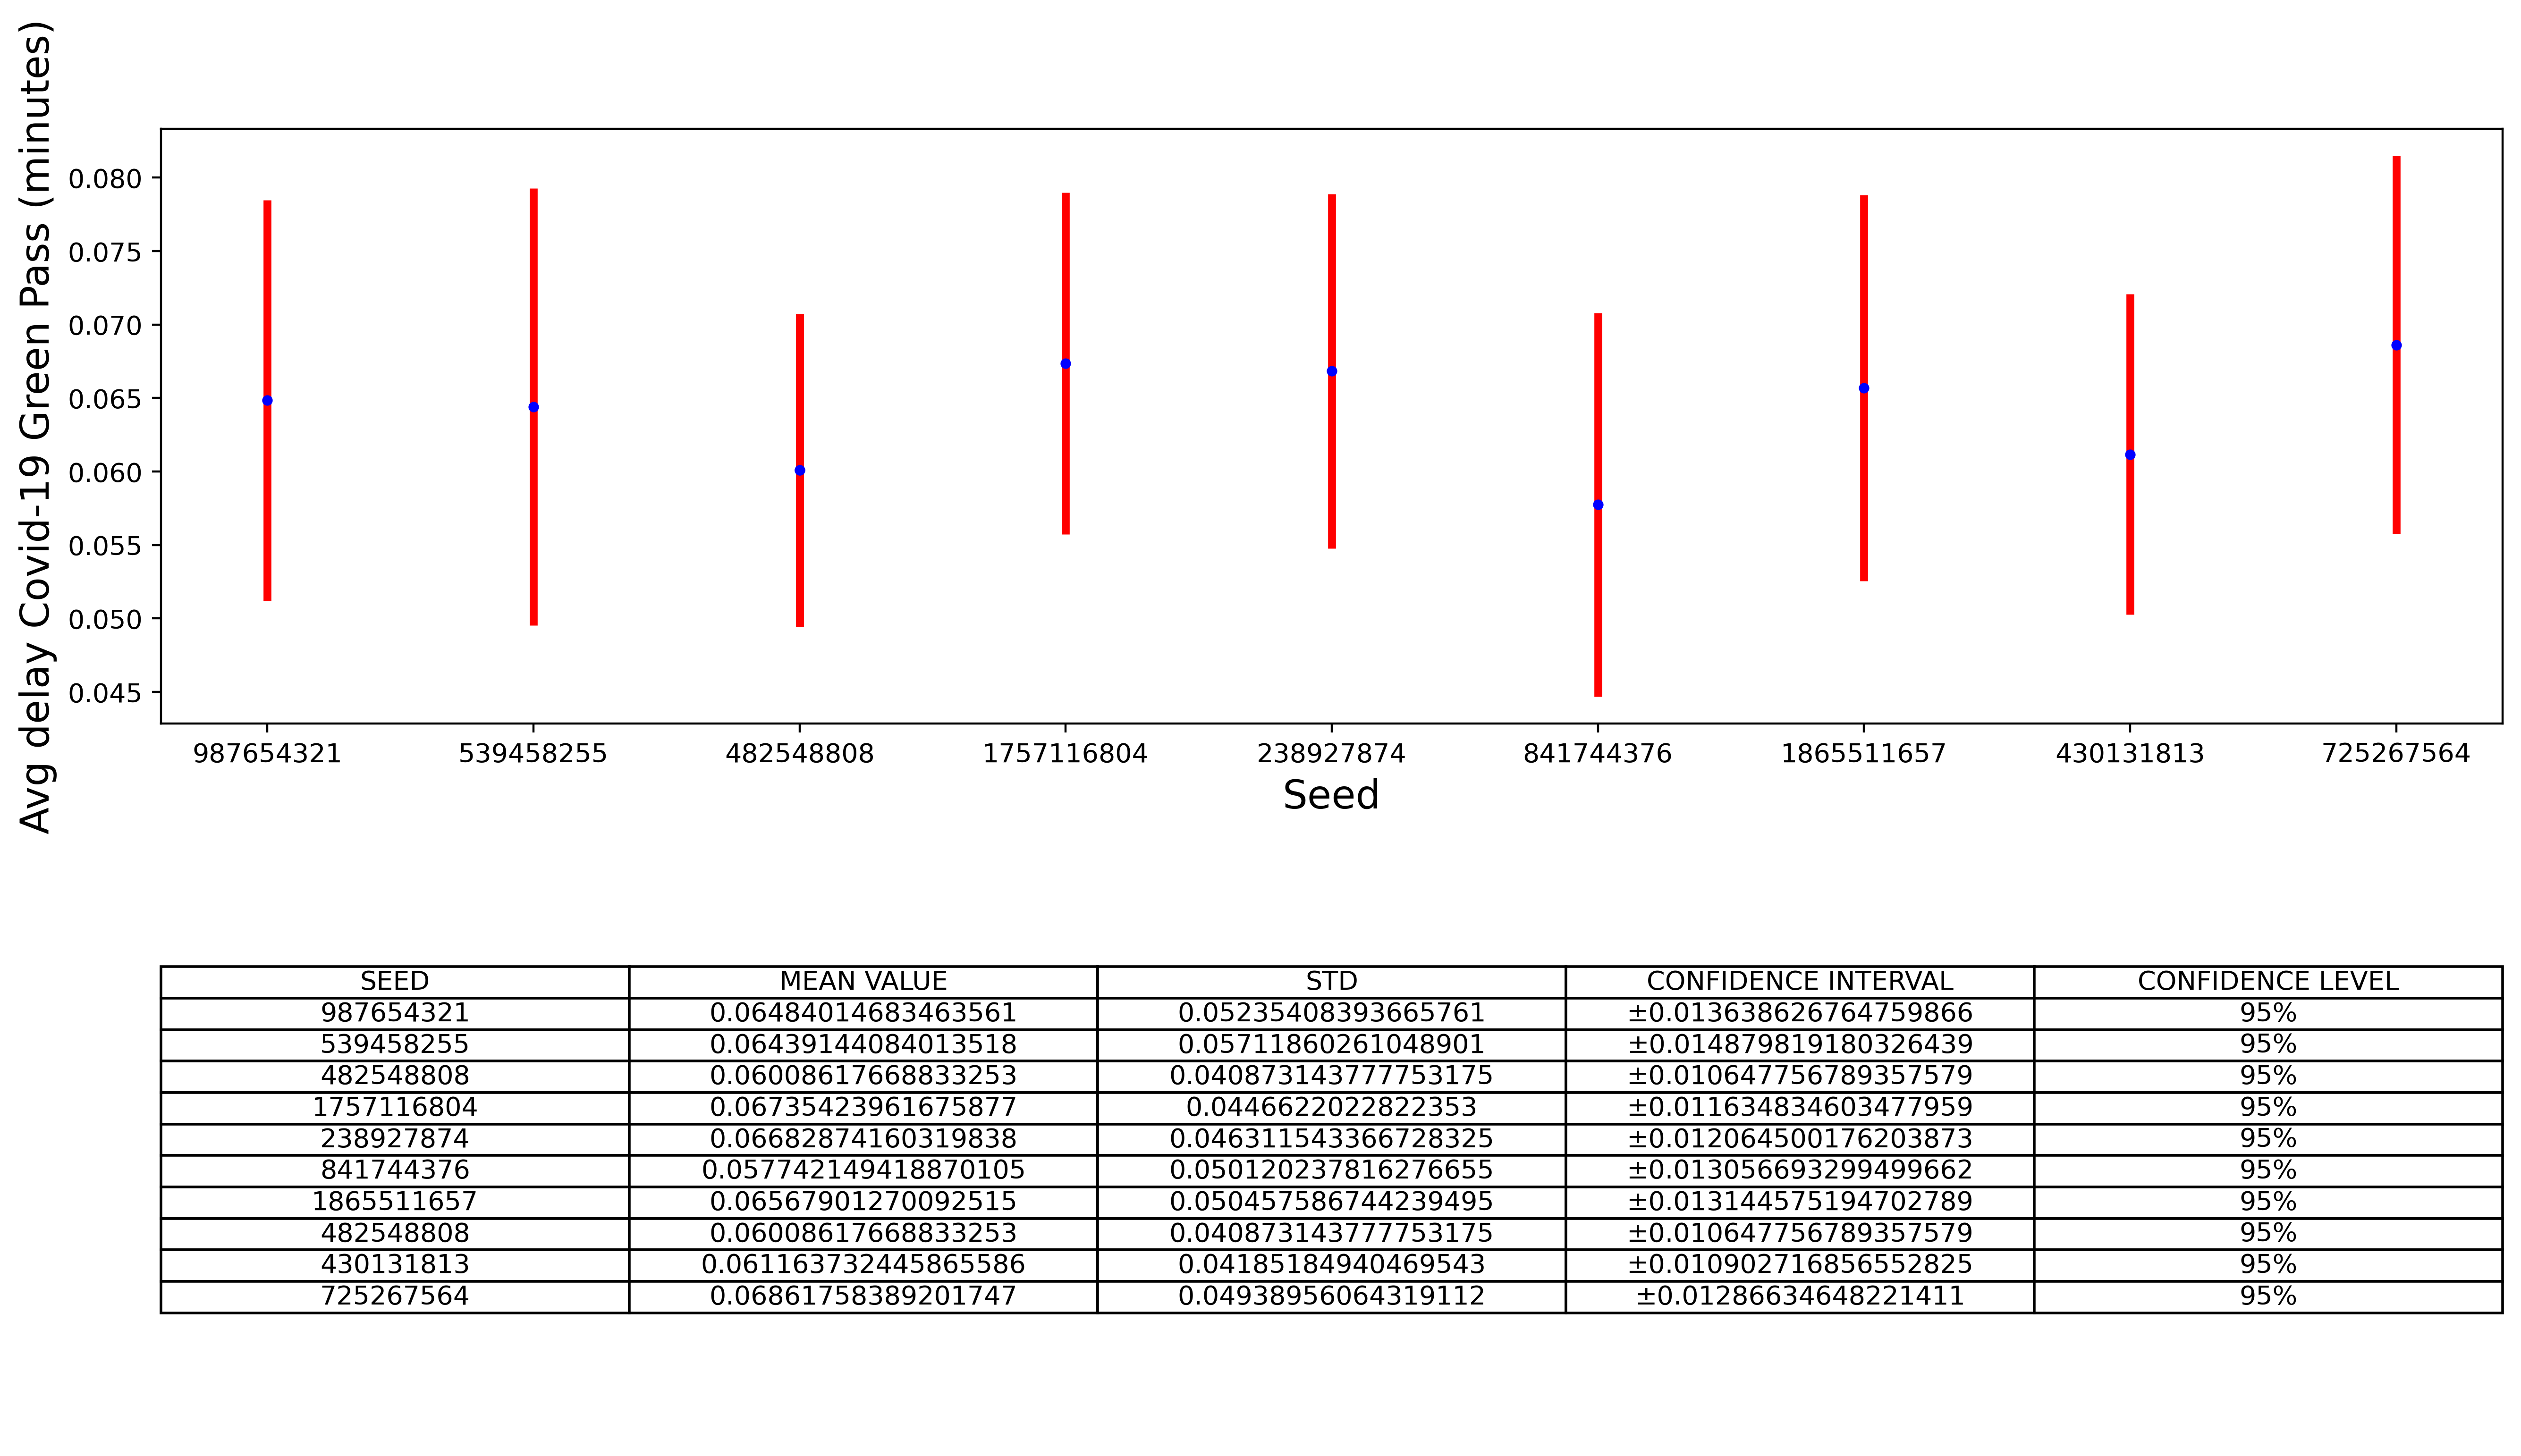
\includegraphics[scale=0.48]{images/adv_avg_d_covid_steady_state_night.png}
	\caption{Advanced Model, Average delay Covid-19 Green-Pass, 22:00-08:00, $\lambda_{arrival}=\frac{1}{35} \frac{job}{min}$, b=256, k=64}\label{figura:adv_avg_d_covid_steady_state_night}
\end{figure}

Come si può osservare dai grafici e dalle tabelle riportate, il tempo di attesa medio nella coda Covid-19, per i clienti che possiedono il Green-Pass, diminuisce sensibilmente utilizzando il modello avanzato, a parità di configurazione e fascia oraria. Tale risultato permette di raggiungere il secondo obiettivo prefissato relativo al modello avanzato.


\subsubsection{Analisi guadagno giornaliero}
Attraverso questa analisi viene effettuata una simulazione concreta di una tipica giornata lavorativa, ricavata nello studio precedente.

\begin{figure}[H]
	\centering
	\captionsetup{justification=centering,margin=2cm}
	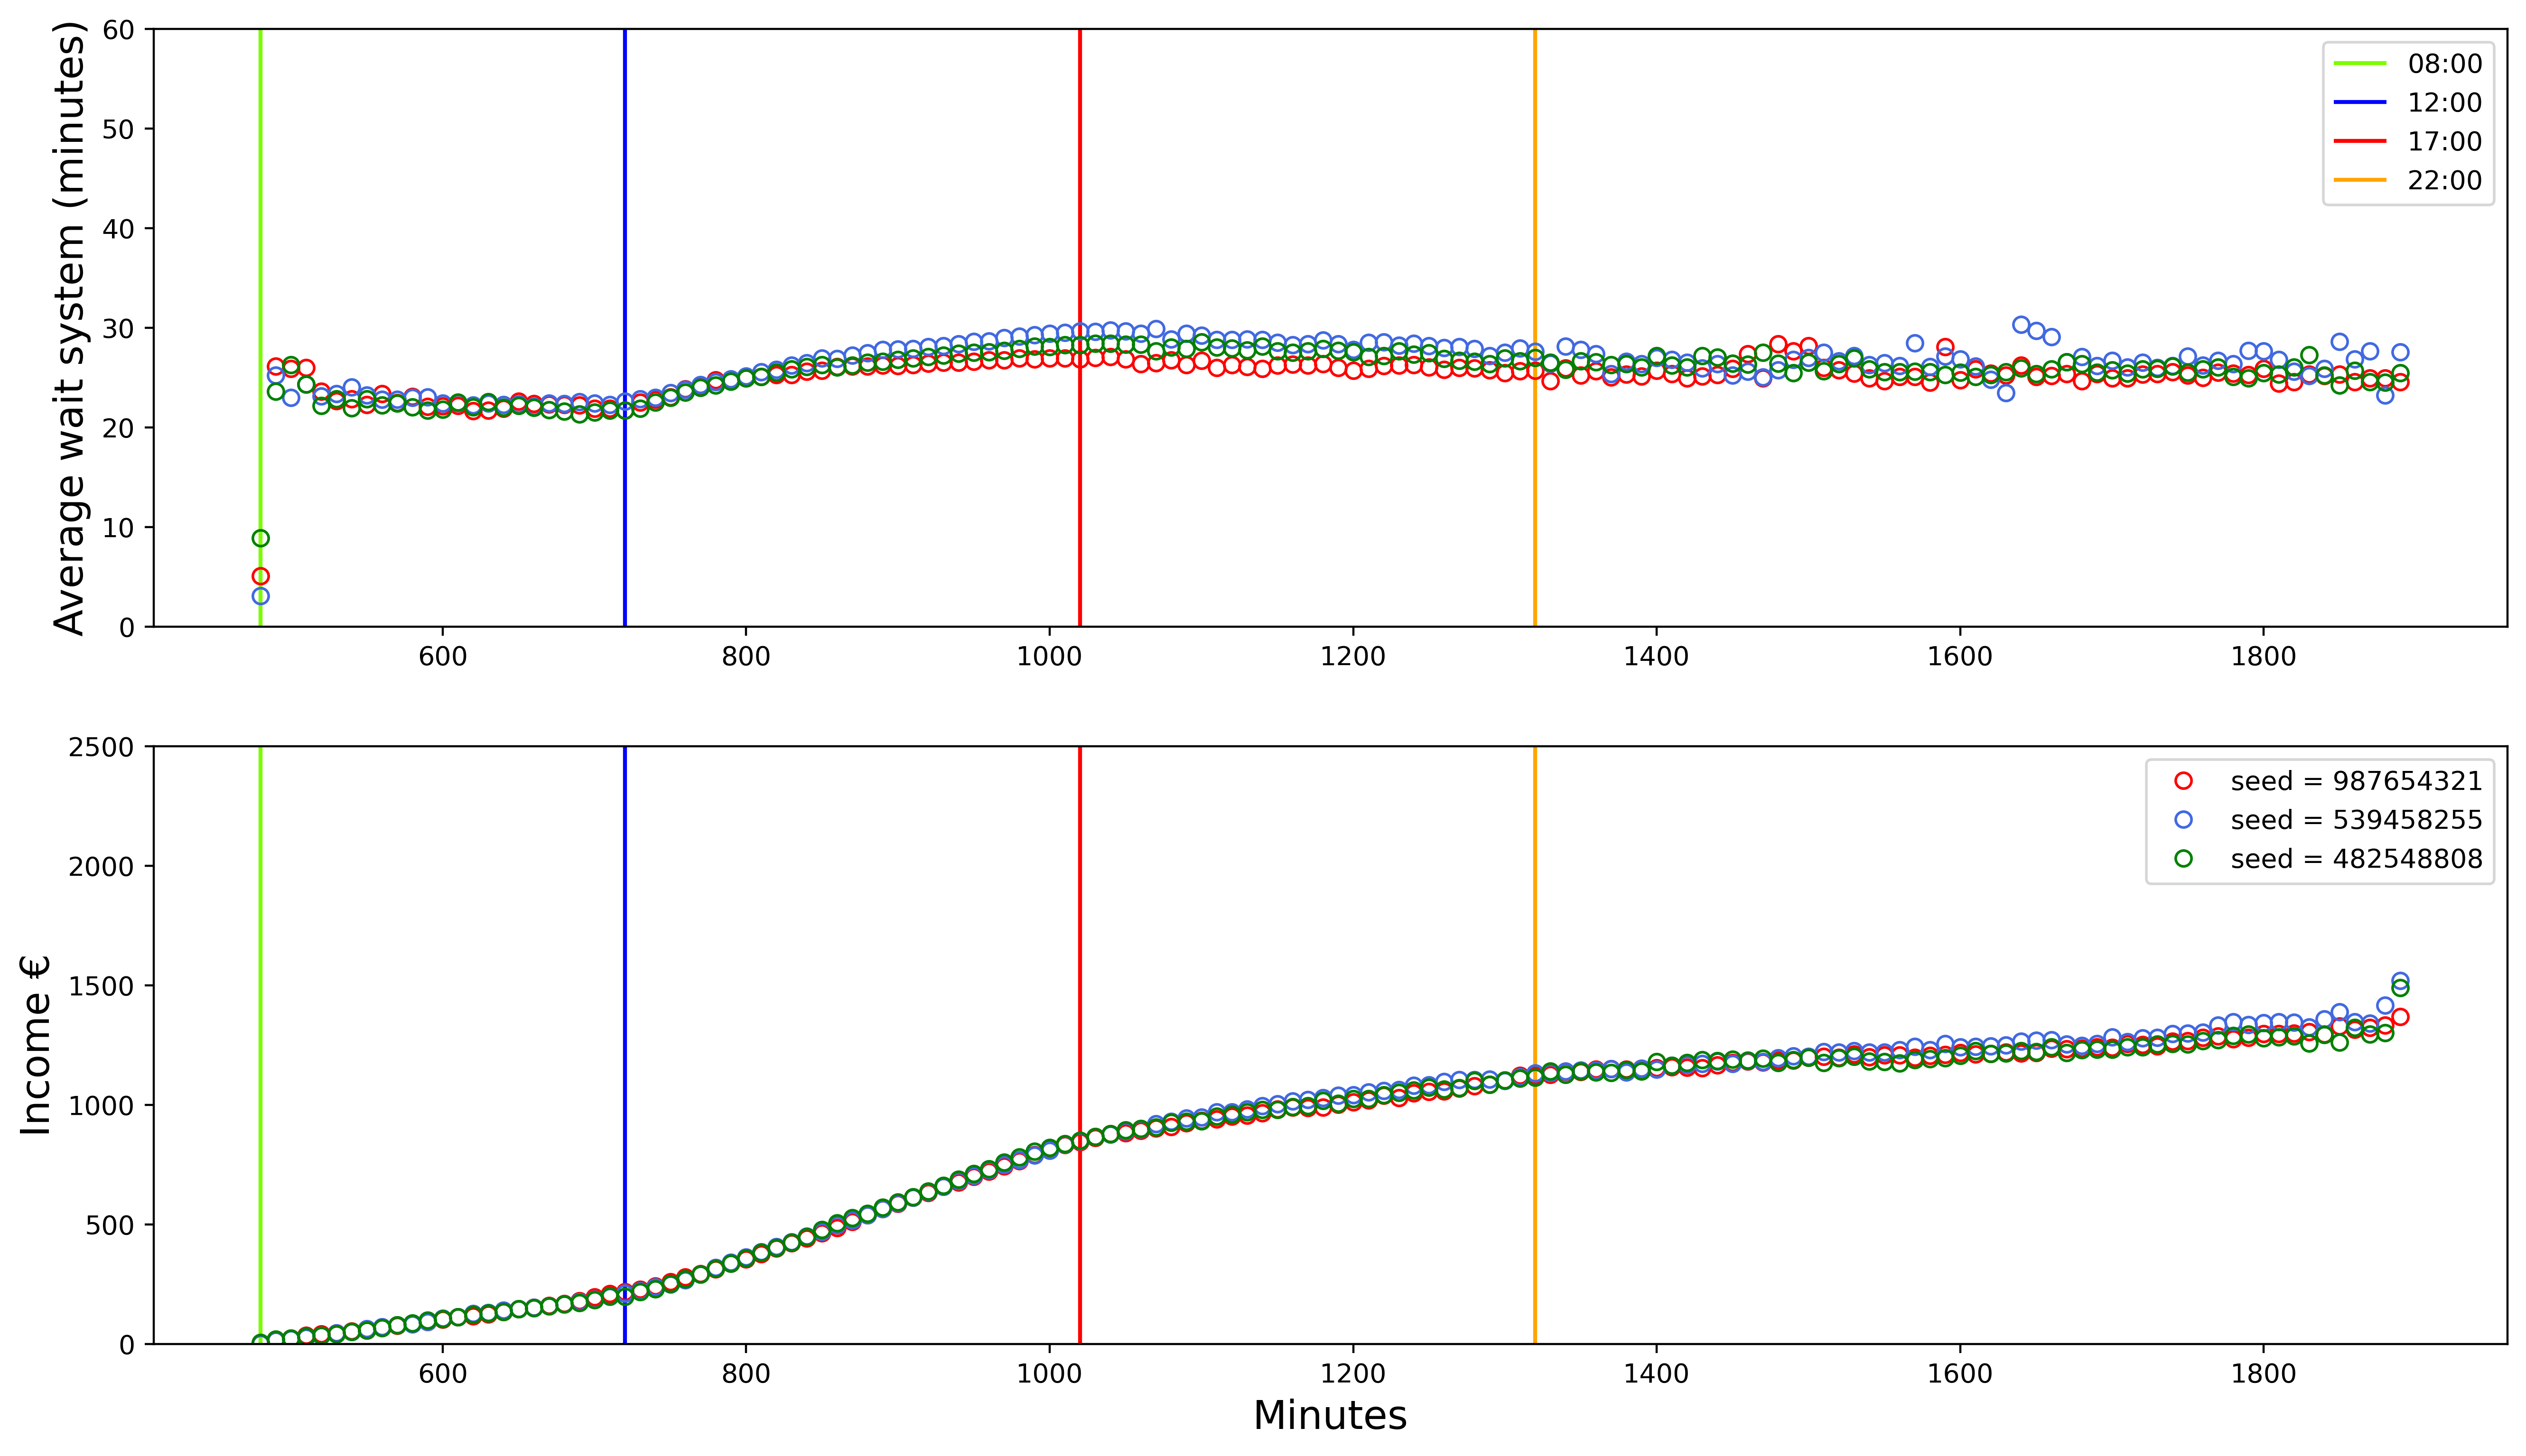
\includegraphics[scale=0.48]{images/ts_optimal_confronto.png}
	\caption{Average Wait System \& Income Daily, Base Model, best configuration, sampling frequency=10 min}\label{figura:ts_optimal_1}
\end{figure}
\begin{figure}[H]
	\centering
	\captionsetup{justification=centering,margin=2cm}
	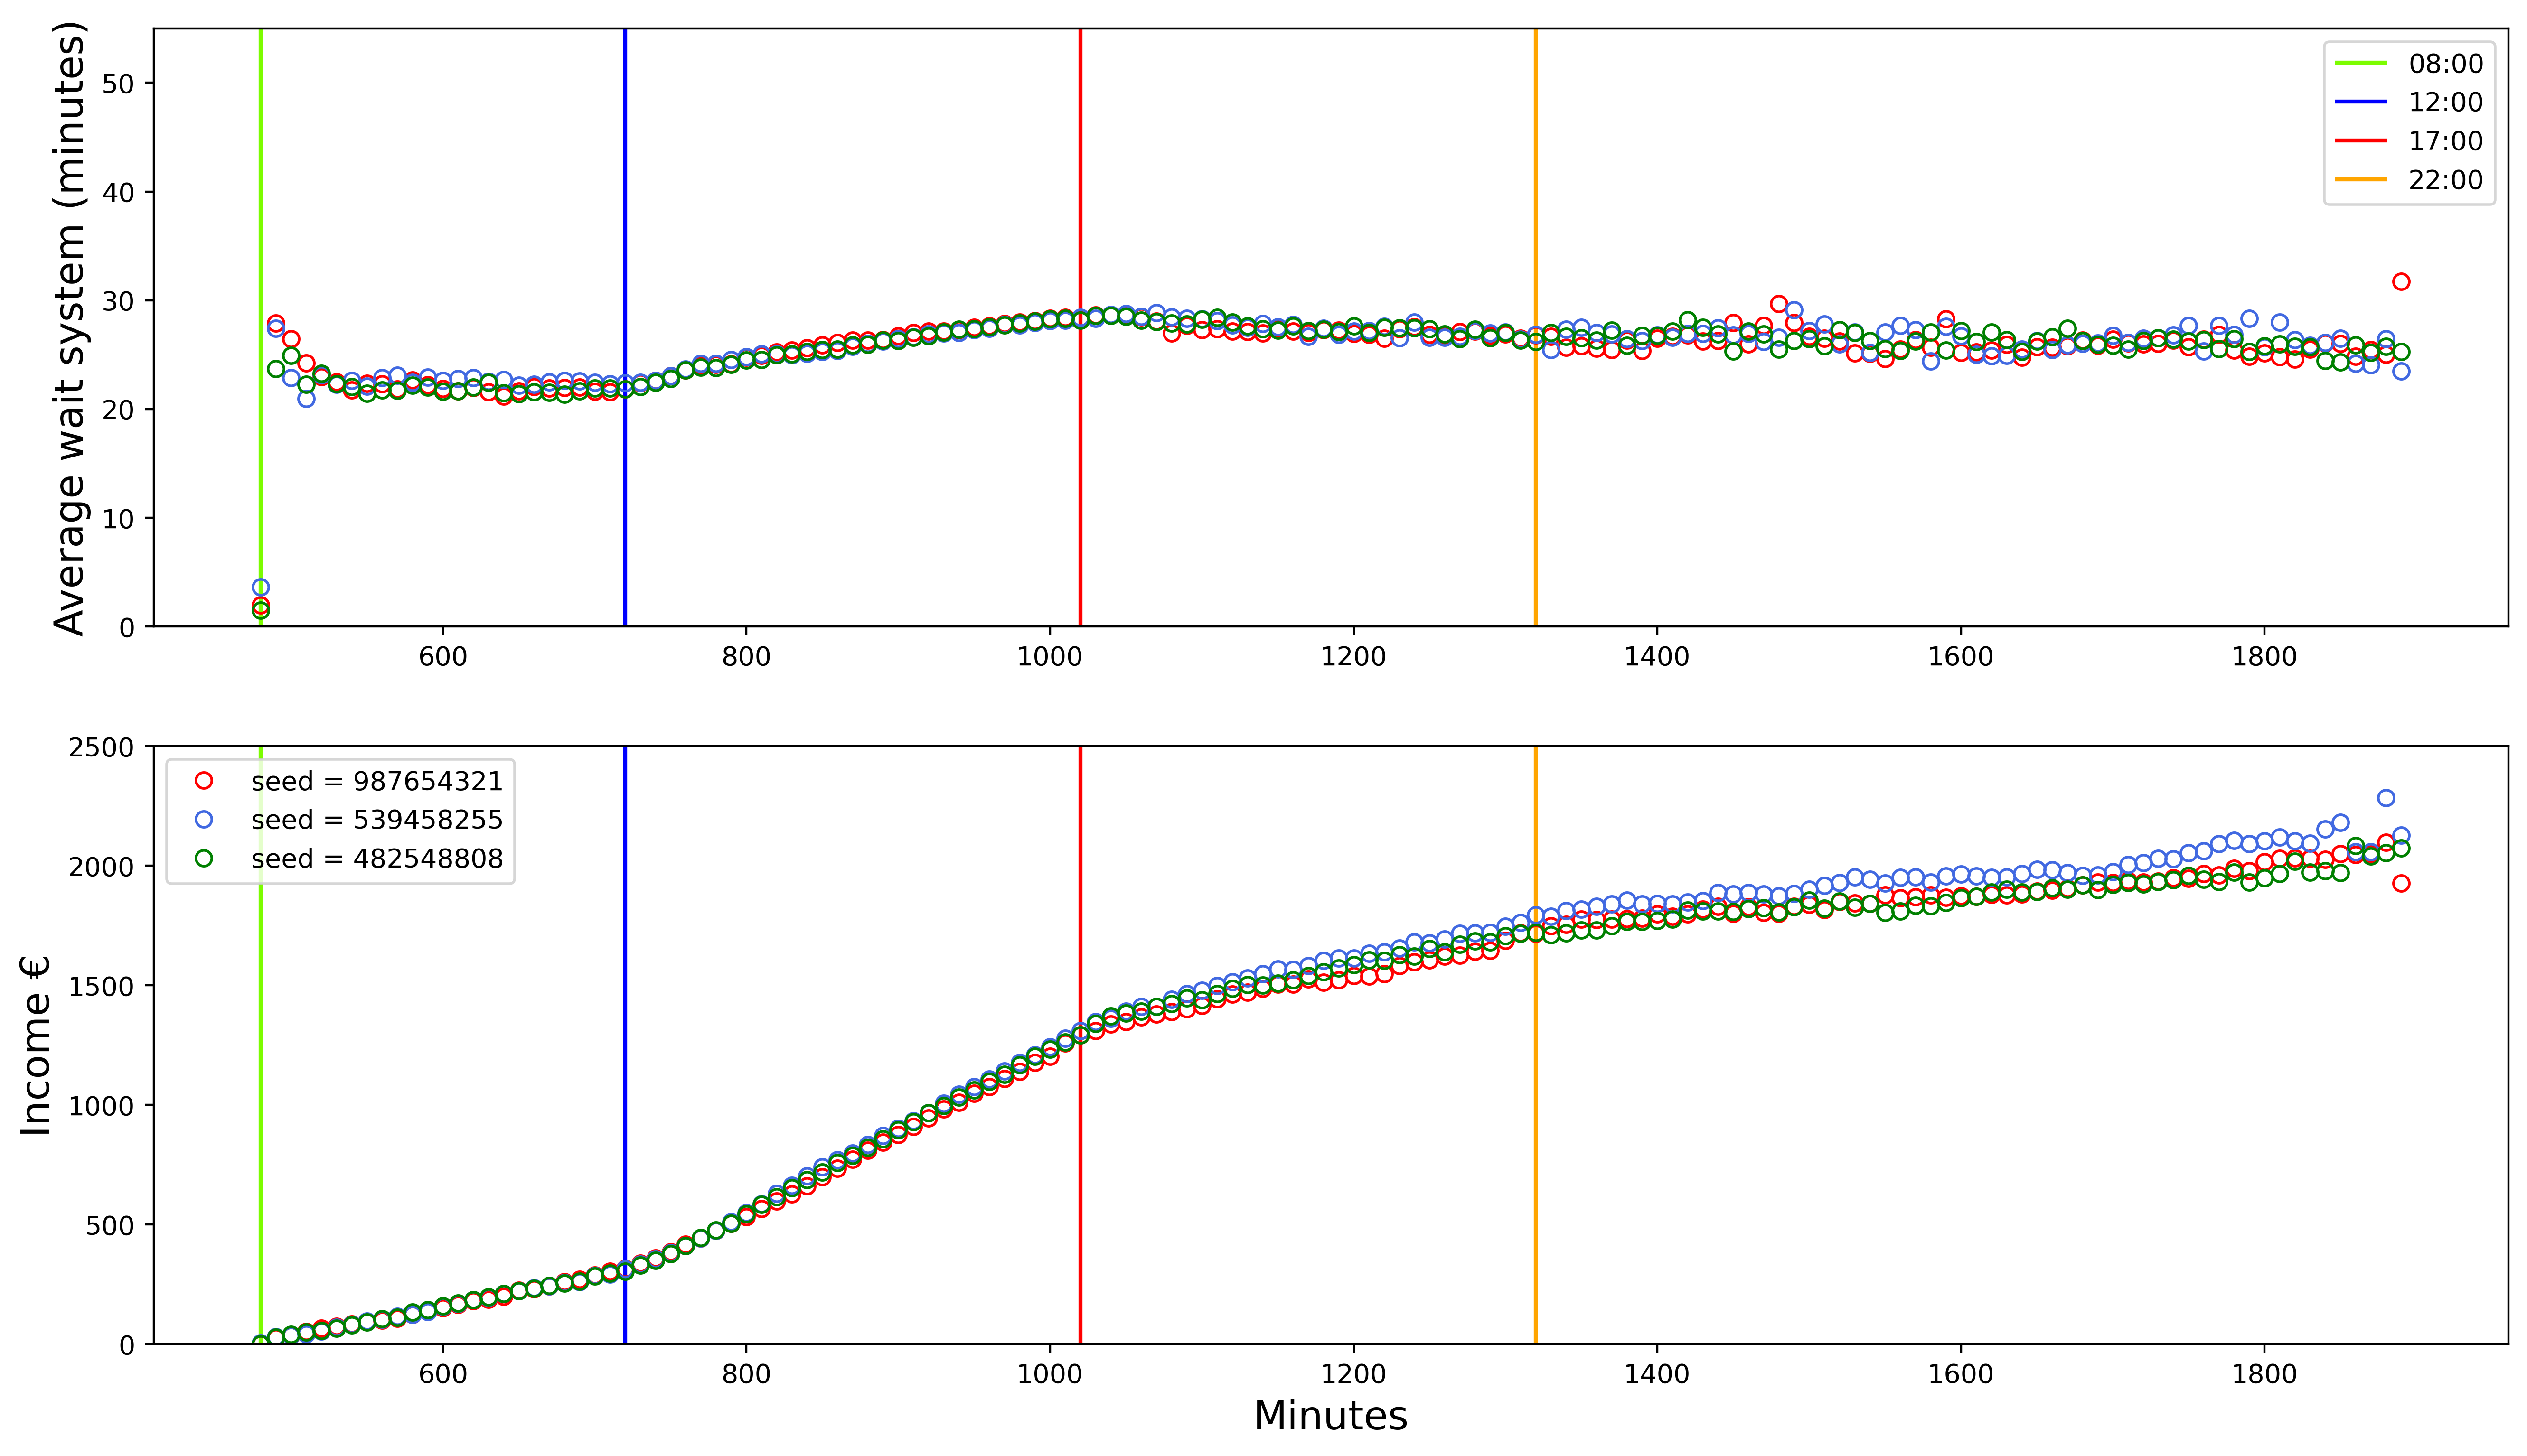
\includegraphics[scale=0.48]{images/adv_ts_optimal.png}
	\caption{Average Wait System \& Income Daily, Advanced Model, best configuration, sampling frequency=10 min}\label{figura:adv_ts_optimal}
\end{figure}

Nelle figure \ref{figura:ts_optimal_1} e \ref{figura:adv_ts_optimal} si può notare il confronto tra il modello base e quello avanzato in corrispondenza della configurazione ottimale. In particolare si osserva un aumento del guadagno, nel caso avanzato, semplicemente introducendo code di priorità, senza incrementare il numero di nodi o i tempi di servizio. Inoltre, si ottiene, mediamente, un tempo di risposta medio del sistema pari o minore a quello del modello base, per via dell'introduzione della priorità basata sulla size per quanto riguarda il nodo Covid-19, nonostante quest'ultima impatti poco sul sistema stesso. Questa analisi conduce al raggiungimento del primo obiettivo.

\section{Conclusioni}

L'intento principale dell'analisi è quello di massimizzare i profitti di una sala giochi, individuando la configurazione ottimale del sistema con lo studio del modello base. Successivamente, attraverso lo studio del modello avanzato, si è agito sulla struttura della rete, in modo da evitare ulteriori spese dovute all'introduzione di centri aggiuntivi. Inoltre, viene adottata una politica più fair nei confronti dei clienti provvisti di green-pass; infatti, questi sperimentano un tempo di attesa in coda proporzionale al tempo di servizio. 

\begin{thebibliography}{00}
\bibitem{b1} Lawrence M. Leemis, Sthephen K. Park, Discrete-Event Simulation - A first course, Pearson Education Prentice Hall,
2006.
\bibitem{b2} \url{https://github.com/pdsteele/DES-Python} \label{link}
\end{thebibliography}
 
%----------------------------------------------------------------------------------------

\end{document}
